\documentclass[14pt]{extarticle}
\usepackage[utf8]{inputenc}
\usepackage{amsmath}
\usepackage{amsfonts}
\usepackage{graphicx}
\usepackage{setspace}
\usepackage{geometry}
\usepackage{enumitem}
\usepackage{amssymb}
\usepackage{xcolor}
\usepackage{mathtools}
\usepackage{float}
\usepackage{listings}
\usepackage{tabularx}
\usepackage{booktabs}

\geometry{
    top=1in,
    bottom=1in,
    left=1in,
    right=1in,
    headheight=14pt,
    headsep=25pt,
    footskip=30pt
}
\definecolor{darkgreen}{rgb}{0.0, 0.5, 0.0}

\title{Bayes Theorem}
\author{Yana Jin}
\date{Wednesday, 24th September 2024}

\onehalfspacing

\newcommand{\coverpage}{%
    \begin{titlepage}
        \centering
        
\includegraphics[width=1\textwidth]{cover.png}
    \end{titlepage}
}

\begin{document}

\coverpage

\section*{Complex Regressors}

\subsection*{Factors}

\noindent
\textbf{One-Factor Models}
\begin{figure}[H]
    \centering
    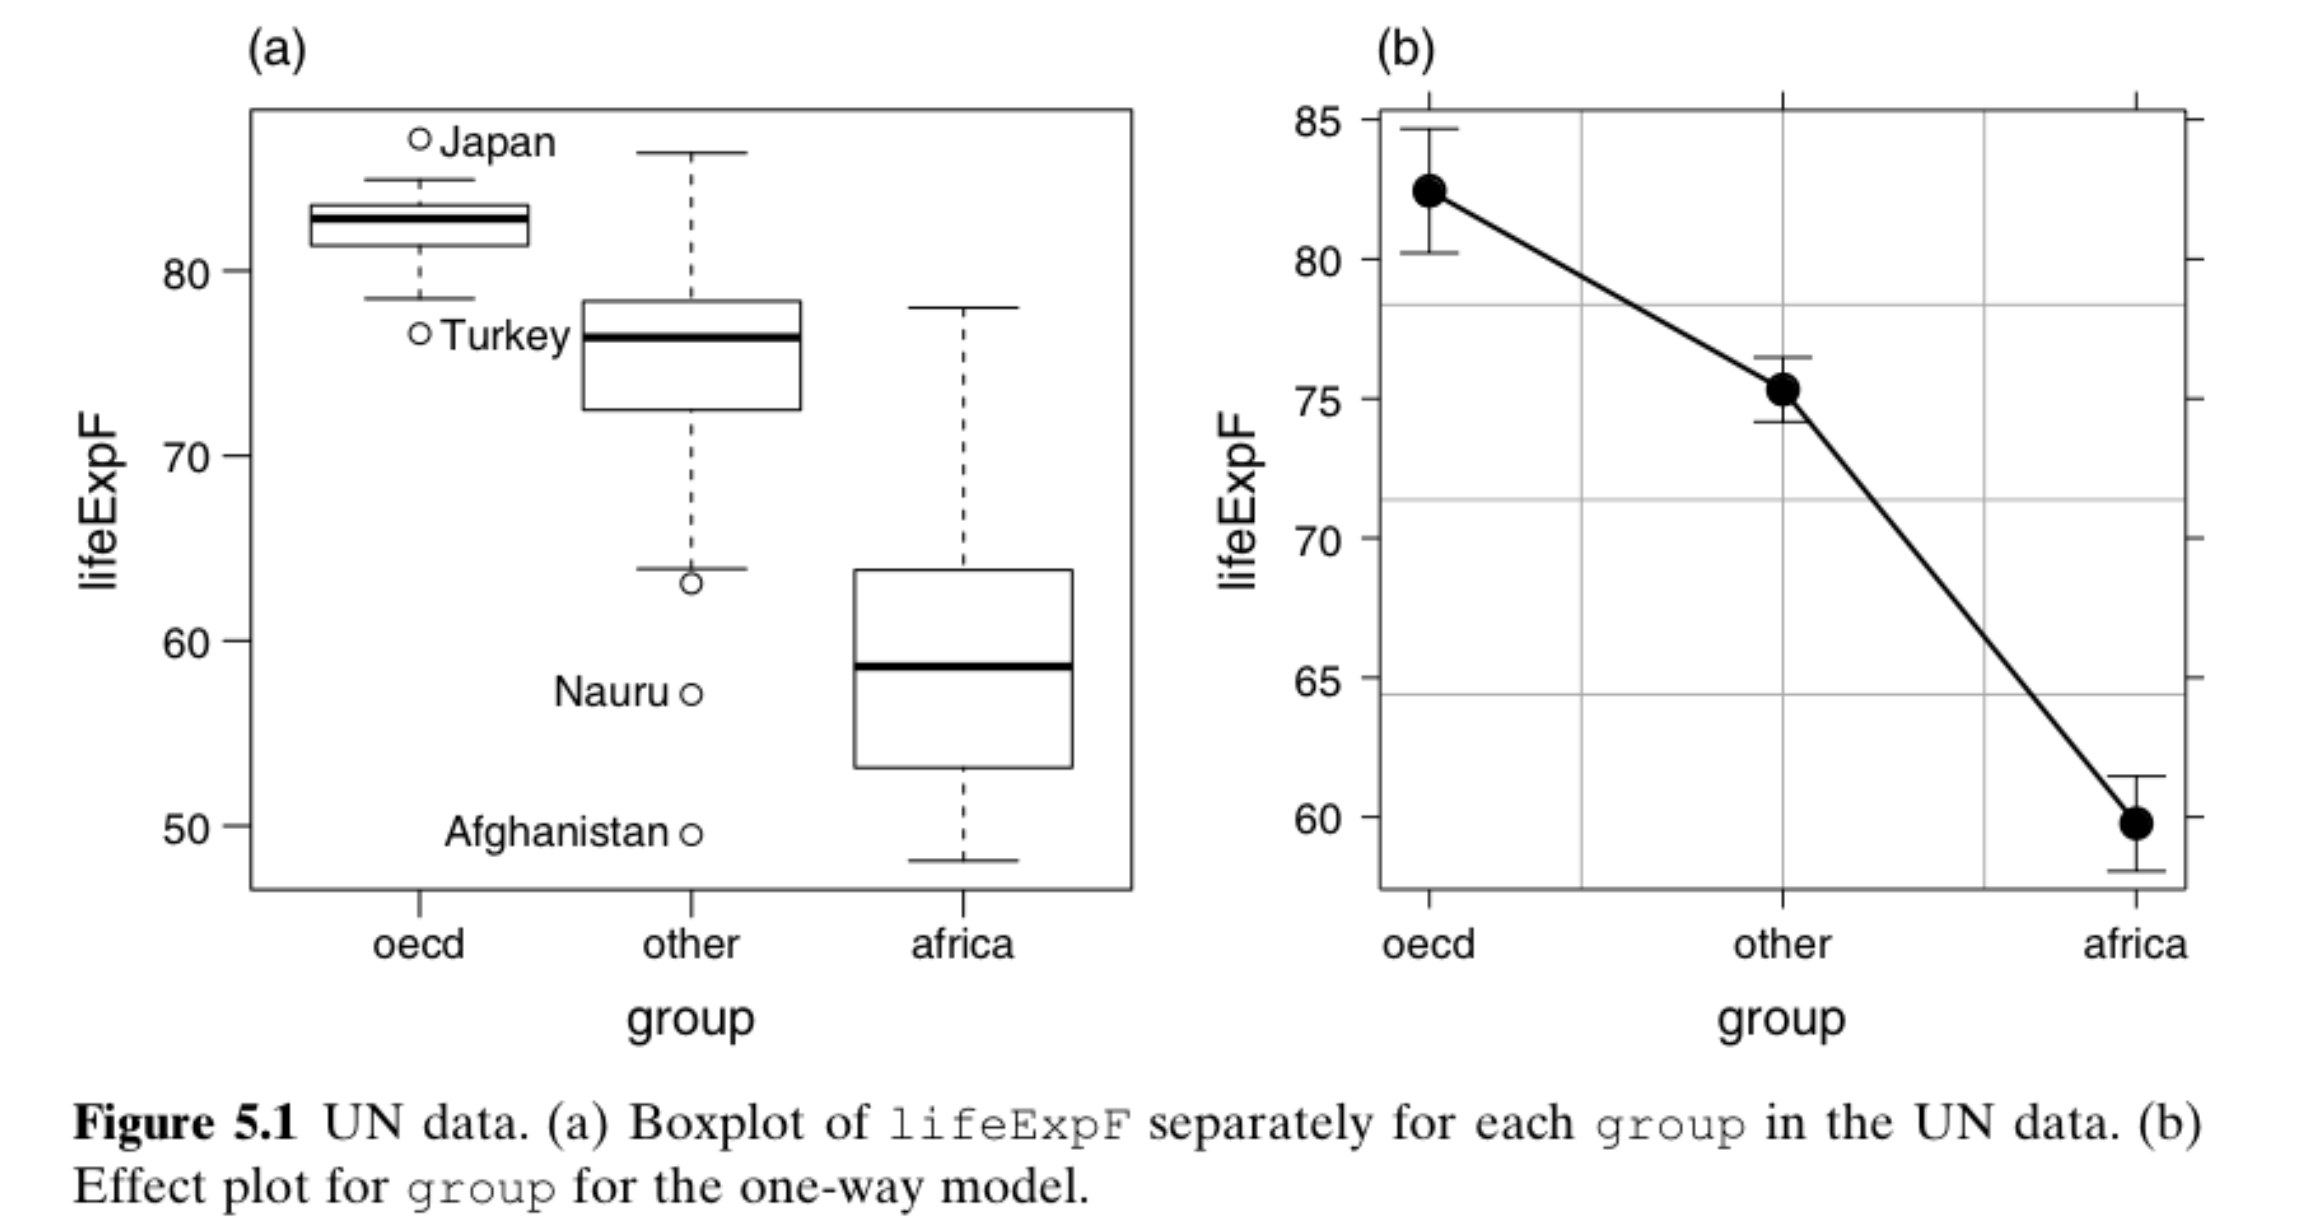
\includegraphics[width=1\textwidth]{fig1.png}
\end{figure}
- when no other predictor in model other than \textcolor{blue}{group}.\\
We model factors using \textcolor{blue}{dummy variables}.\\
Factor with \(k\) levels, has $(k - 1)$ dummy variables.\\
\textcolor{blue}{Example: For $j^{th}$ dummy variable $u_{ij}, j=1,\dots,d$, has $i^{th}$ value $u_{ij}$ for $i = 1, \dots, n$:
\[
u_{ij} = 
\begin{cases} 
1 & \text{, if group } i = j\text{th category} \\
0 & \text{, otherwise}
\end{cases}
\]}

\newpage

\noindent
The values of the dummy variables for the first 10 cases in the example are as follows:\vspace{0.2cm}

\noindent
\begin{tabular}{lcccc}
\toprule
\textbf{\quad \quad \quad \quad \quad} & \textbf{\quad \quad Group \quad \quad} & $\quad \quad U_1 \quad \quad$ & $\quad \quad U_2 \quad \quad$ & $\quad \quad U_3 \quad \quad$ \\
\midrule
Afghanistan & other & 0 & 1 & 0 \\
Albania     & other & 0 & 1 & 0 \\
Algeria     & africa & 0 & 0 & 1 \\
Angola      & africa & 0 & 0 & 1 \\
Anguilla    & other & 0 & 1 & 0 \\
Argentina   & other & 0 & 1 & 0 \\
Armenia     & other & 0 & 1 & 0 \\
Aruba       & other & 0 & 1 & 0 \\
Australia   & oecd & 1 & 0 & 0 \\
Austria     & oecd & 1 & 0 & 0 \\
\bottomrule
\end{tabular}\vspace{0.2cm}

\noindent
If we add an intercept, \(\Rightarrow\) overparameterized model \\
because \( u_1 + u_2 + u_3 = 1 \) and column of 1's for intercept. \\
\textcolor{red}{Solve this by dropping one of dummy variables.}
\[
E(\text{lifeExpF} | \text{group}) = \beta_0 + \beta_2 U_2 + \beta_3 U_3
\]
Since the first level of group will be implied when \(U_2 = U_3 = 0\),
\[
E(\text{lifeExpF} | \text{group} = \text{oecd}) = \beta_0 + \beta_2 0 + \beta_3 0 = \beta_0
\]
and so \(\beta_0\) is the mean for the first level of \textit{group}. \\
For the second level, \(U_2 = 1\) and \(U_3 = 0\),
\[
E(\text{lifeExpF} | \text{group} = \text{other}) = \beta_0 + \beta_2 1 + \beta_3 0 = \beta_0 + \beta_2
\]
and \(\beta_0 + \beta_2\) is the mean for the second level of \textit{group}. \\
Similarly, for the third level, \(U_2 = 0\) and \(U_3 = 1\),
\[
E(\text{lifeExpF} | \text{group} = \text{africa}) = \beta_0 + \beta_2 0 + \beta_3 1 = \beta_0 + \beta_3
\]
\begin{table}[H]
    \textbf{Table5.1 Regression Summary for Model (5.4)}
    \centering
    \begin{tabular}{lcccc}
    \toprule
     & \textbf{  Estimate  } & \textbf{ Std. Error } & \textbf{ t-Value } & \textbf{ Pr$(>|t|)$ } \\
    \midrule
    (Intercept), $\hat{\beta}_0$ & 82.4465 & 1.1279 & 73.09 & 0.0000 \\
    other, $\hat{\beta}_2$ & -7.1197 & 1.2709 & -5.60 & 0.0000 \\
    africa, $\hat{\beta}_3$ & -22.6742 & 1.4200 & -15.97 & 0.0000 \\
    \bottomrule
    \end{tabular}
    $\hat{\sigma} = 6.2801 \text{ with } 196 \text{ df, } R^2 = 0.6191$
\end{table}
\noindent
\textbf{Means for three groups are:}
\[
\hat{E}(\text{lifeExpF} | \text{group=oecd}) = \hat{\beta}_0 + \hat{\beta}_2 \cdot 0 + \hat{\beta}_3 \cdot 0 = 82.45
\]
\[
\hat{E}(\text{lifeExpF} | \text{group=other}) = \hat{\beta}_0 + \hat{\beta}_2 \cdot 1 + \hat{\beta}_3 \cdot 0 = 82.45 - 7.12
\]
\[
\hat{E}(\text{lifeExpF} | \text{group=africa}) = \hat{\beta}_0 + \hat{\beta}_2 \cdot 0 + \hat{\beta}_3 \cdot 1 = 82.45 - 22.67
\]    

\section*{Comparison of Level Means}

With analysis of factors, we often care about comparison of means (adjusted for other factors and regressors).\\
Pairwise comparisons of means:\\
 - requires SE of the differences between each pair of means.\\
\textbf{Example:} Comparing \textcolor{blue}{other} to \textcolor{blue}{africa}
\[
\hat{\beta}_2 - \hat{\beta}_3 = -7.12 - (-22.67) = 15.55
\]
SEs for this difference can be calculated.\\
Let $a = (0, 1, -1, 0)'$
\[
\Rightarrow \ell = a' \beta = \beta_2 - \beta_3 \quad \text{(contrast)}
\]
\[
SE(\hat{\ell} | X) = \hat{\sigma} \sqrt{ a' (X'X)^{-1} a }
\]
\[
= \hat{\sigma} \underbrace{\sqrt{ C_{22} + C_{33} - 2 C_{23} }}_{\textcolor{red}{C_{ij} \text{ is the } (i,j)^{th} \text{ element of } (X'X)^{-1}}}
\]
Then use $t$-value (t-test) to generate $p$-value:
\[
\frac{\hat{\ell}}{SE(\hat{\ell})} \overset{H_0}{\sim} t_{n - (p + 1)}
\]
\begin{table}[H]
\textbf{Table5.2 Pairwise Comparisons of Level Means for Group}
\centering
\begin{tabular}{lcccc}
\toprule
\textbf{Compariso $\quad$} & \textbf{$\quad$Estimate$\quad$} & \textbf{$\quad$SE$\quad$} & \textbf{$\quad$t-Value$\quad$} & \textbf{$\quad$p-Value$\quad$} \\
\midrule
oecd - other  & 7.12  & 1.27 & 5.60  & 0.000 \\
oecd - africa & 22.67 & 1.42 & 15.97 & 0.000 \\
other - africa & 15.55 & 1.04 & 14.92 & 0.000 \\
\bottomrule
\end{tabular}
\end{table}
\begin{figure}[H]
    \centering
    
\includegraphics[width=1\textwidth]{fig2.png}
\end{figure}
\begin{figure}[H]
    \centering
    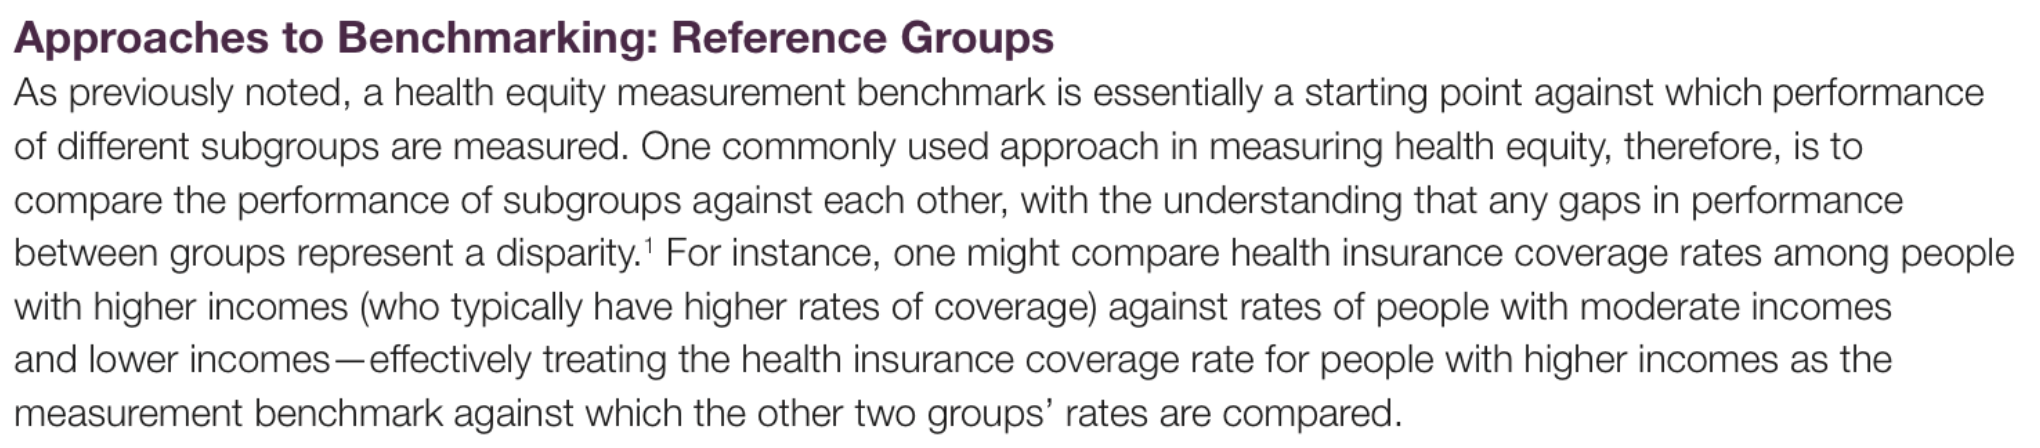
\includegraphics[width=1\textwidth]{fig3.png}
\end{figure}
\begin{figure}[H]
    \centering
    
\includegraphics[width=1\textwidth]{fig4.png}
\end{figure}
\begin{figure}[H]
    \centering
    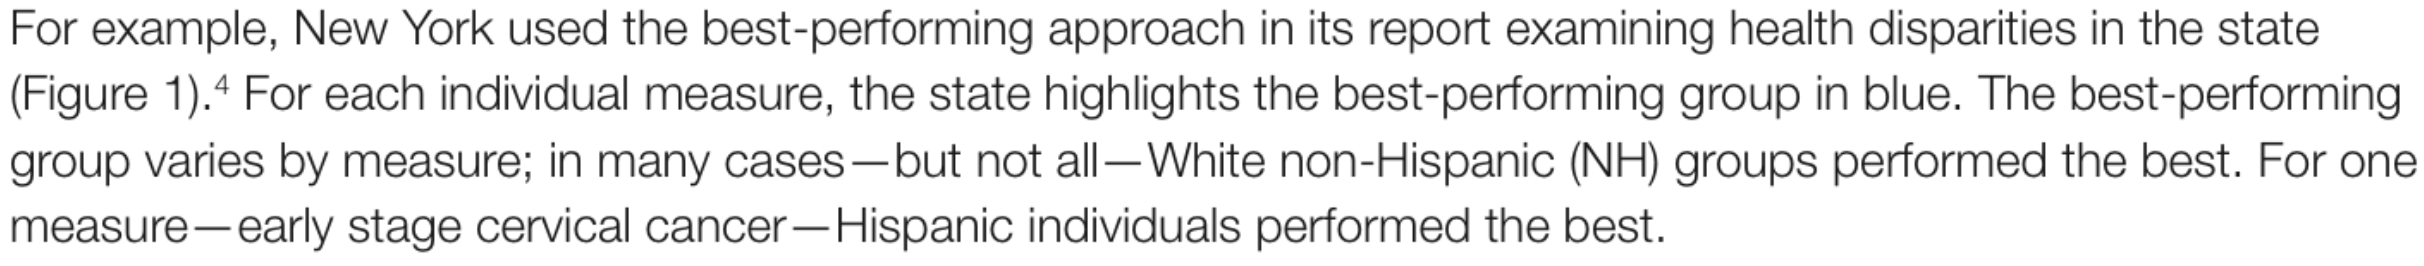
\includegraphics[width=1\textwidth]{fig5.png}
\end{figure}
\begin{figure}[H]
    \centering
    
\includegraphics[width=1\textwidth]{fig6.png}
\end{figure}
\begin{figure}[H]
    \centering
    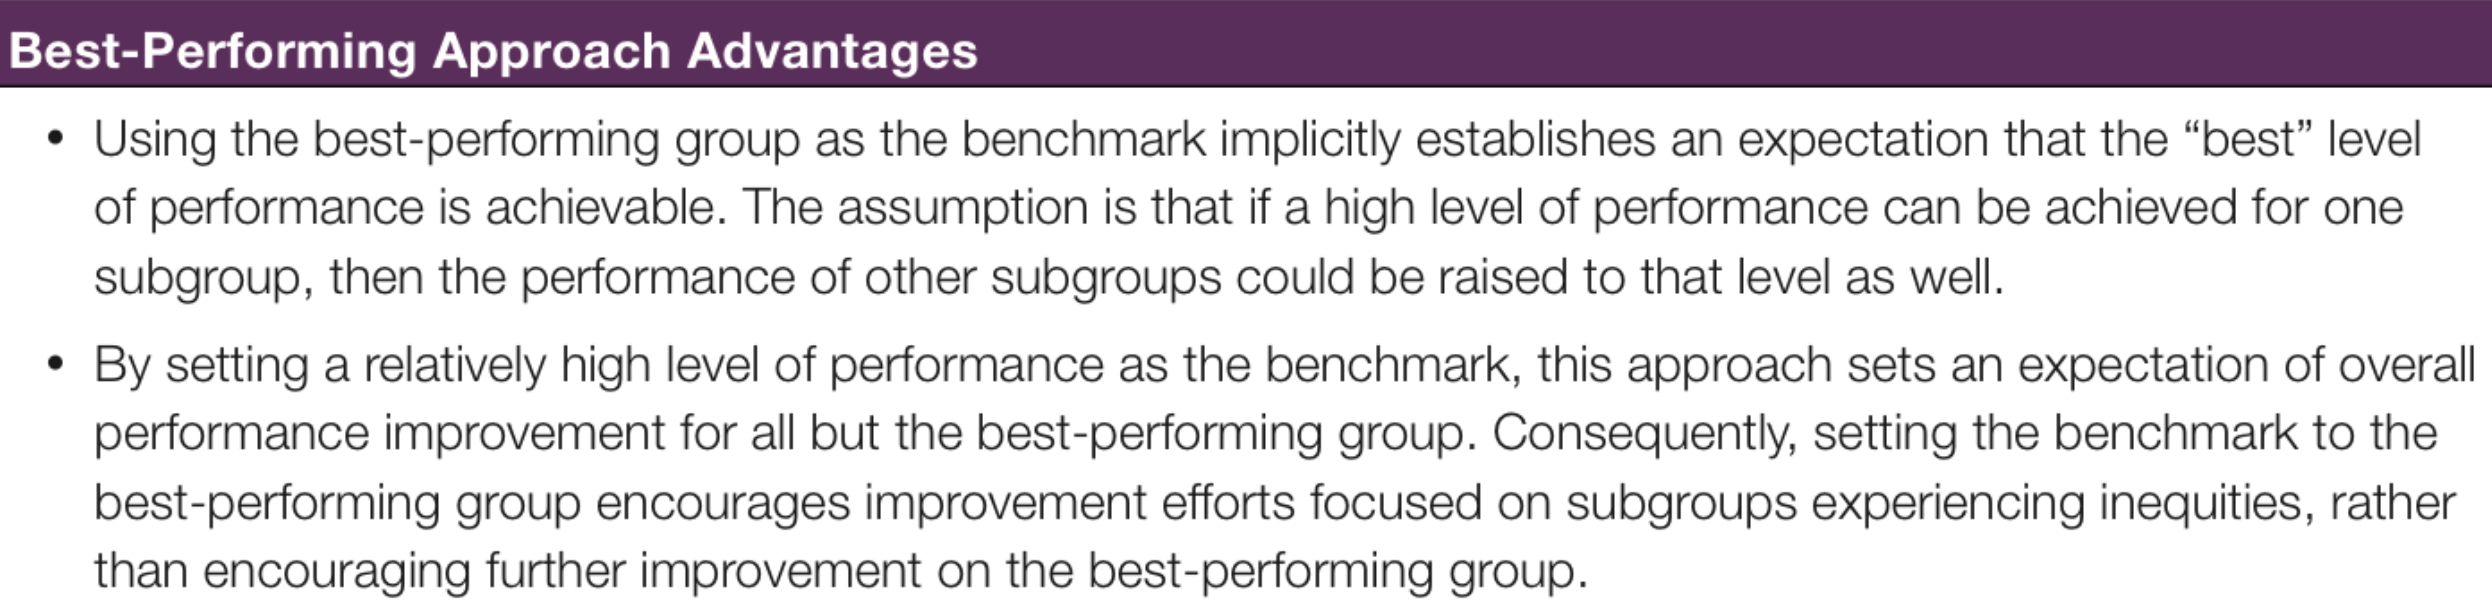
\includegraphics[width=1\textwidth]{fig7.png}
\end{figure}
\begin{figure}[H]
    \centering
    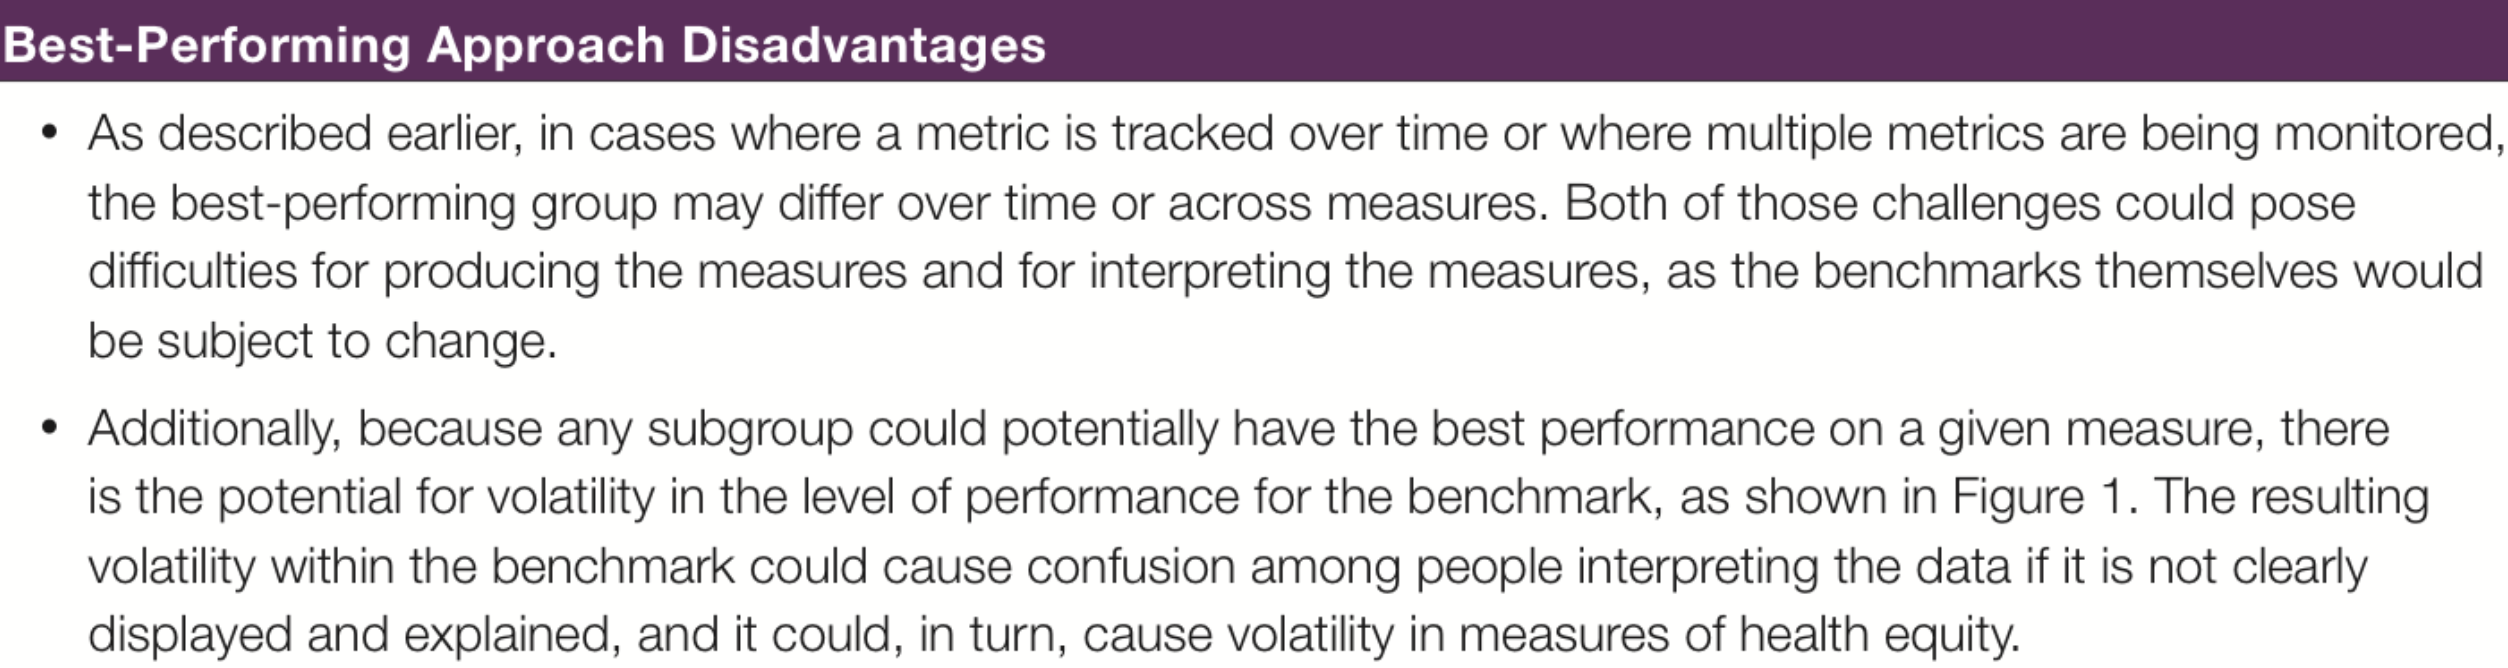
\includegraphics[width=1\textwidth]{fig8.png}
\end{figure}
\begin{figure}[H]
    \centering
    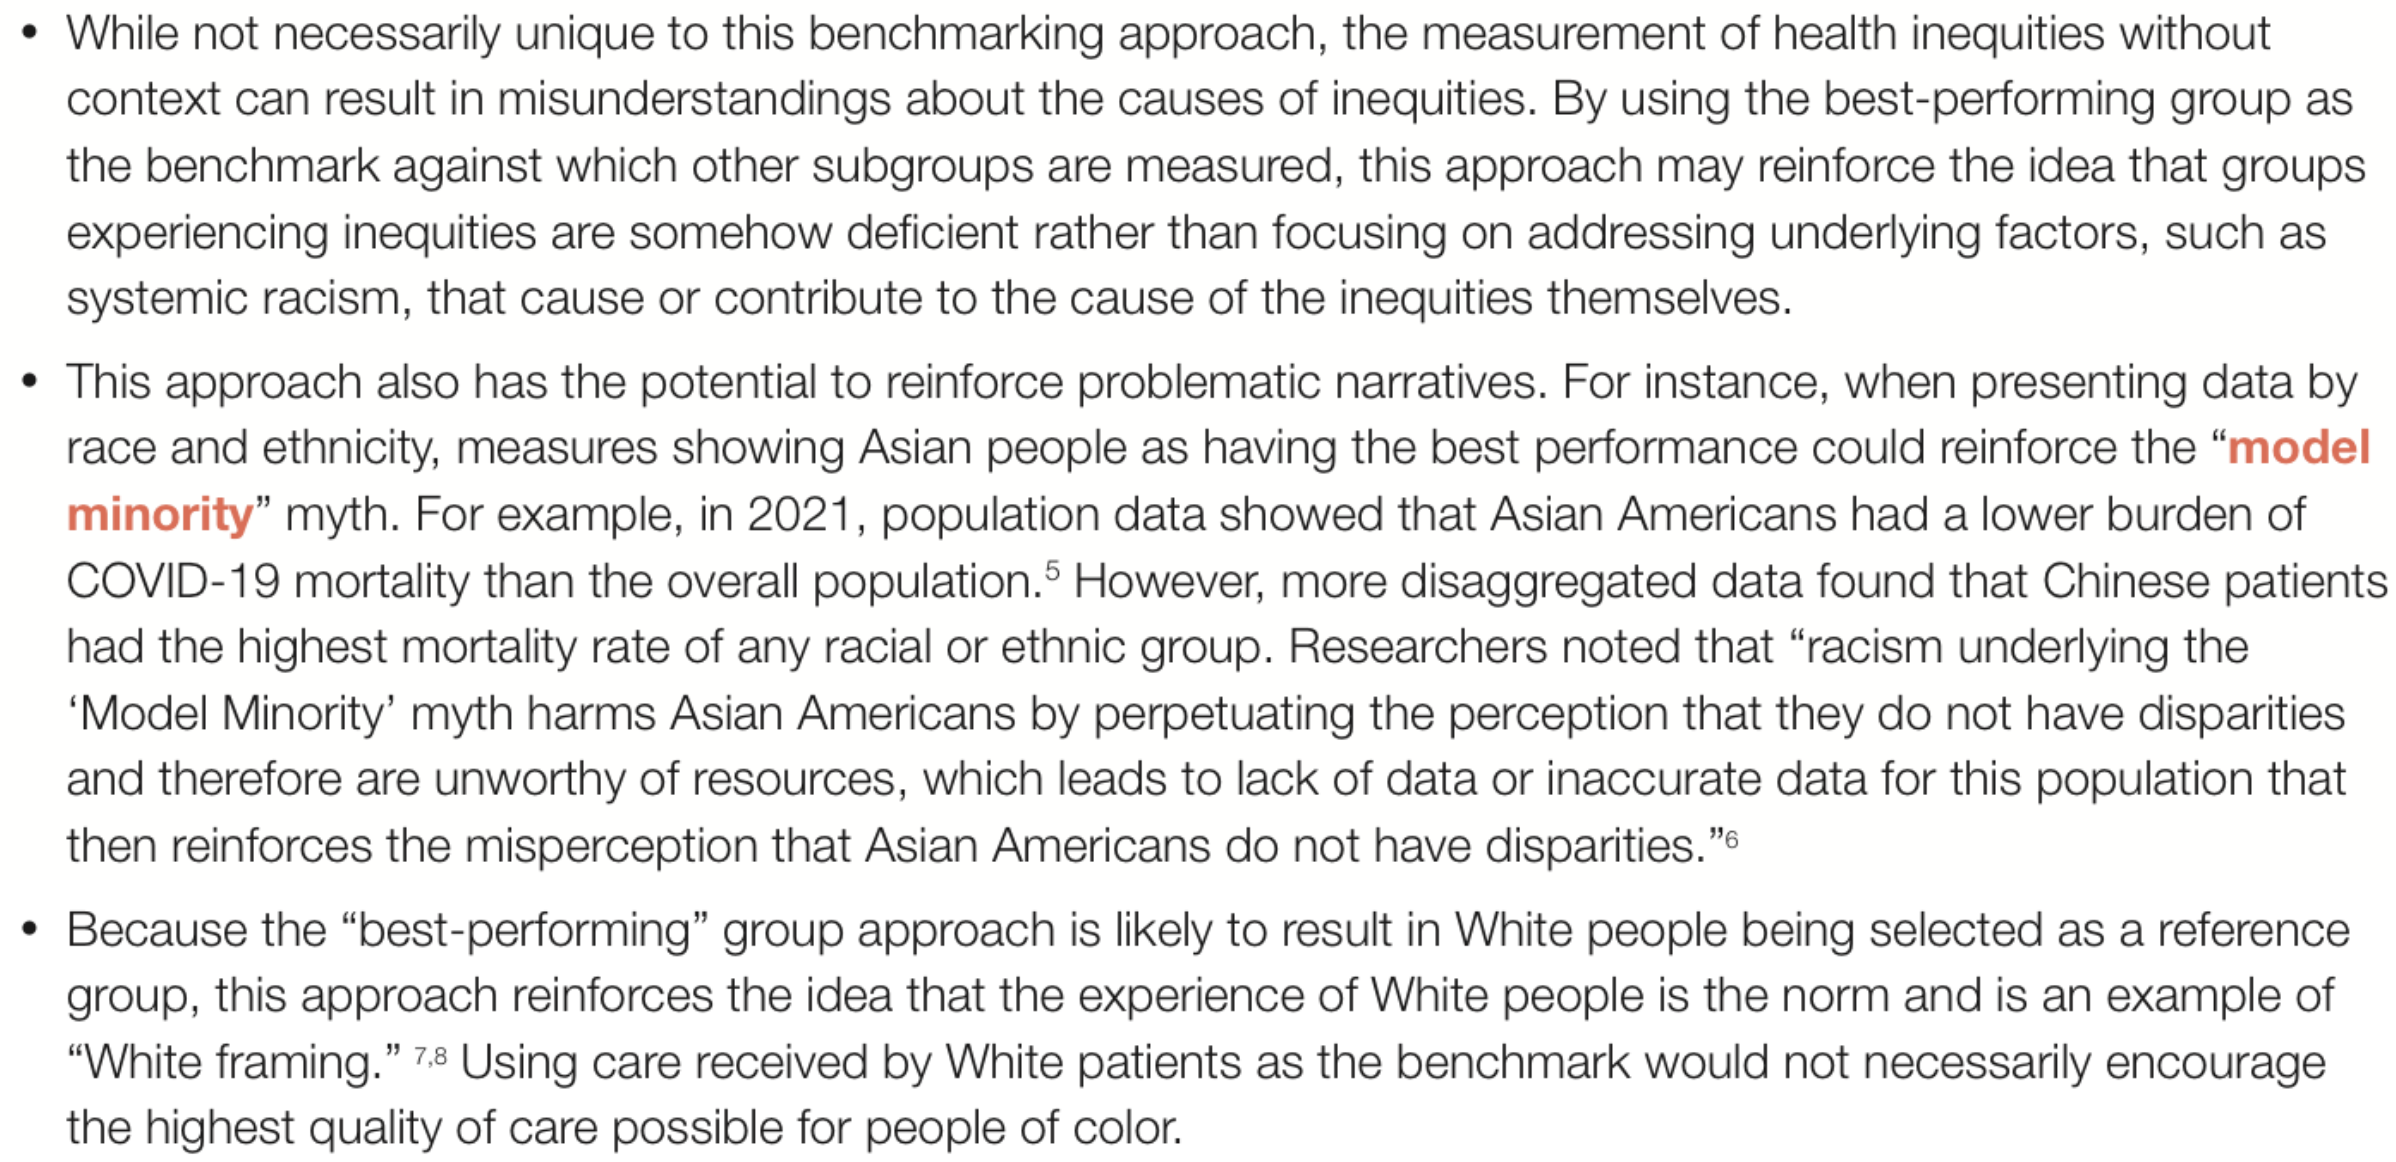
\includegraphics[width=1\textwidth]{fig9.png}
\end{figure}
\begin{figure}[H]
    \centering
    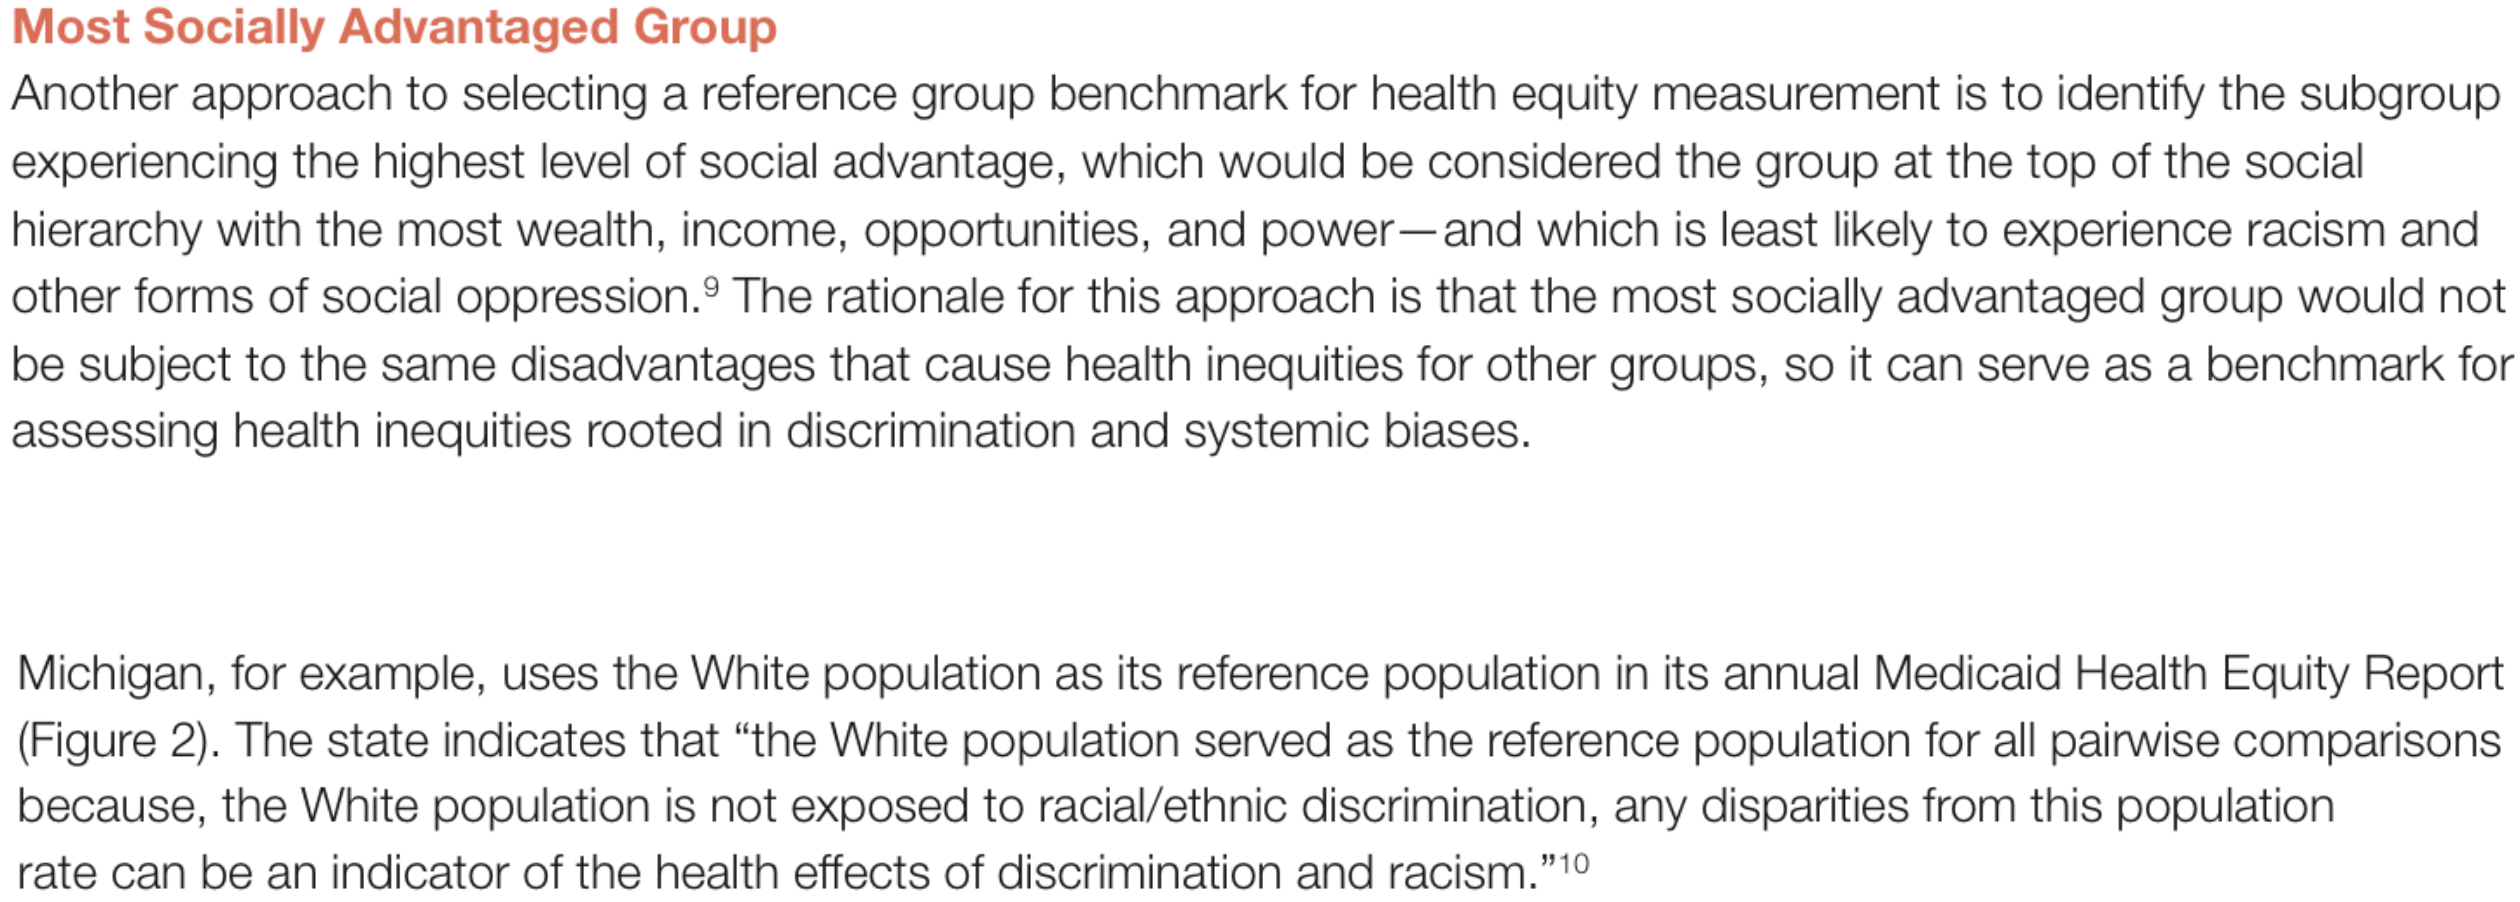
\includegraphics[width=1\textwidth]{fig10.png}
\end{figure}
\begin{figure}[H]
    \centering
    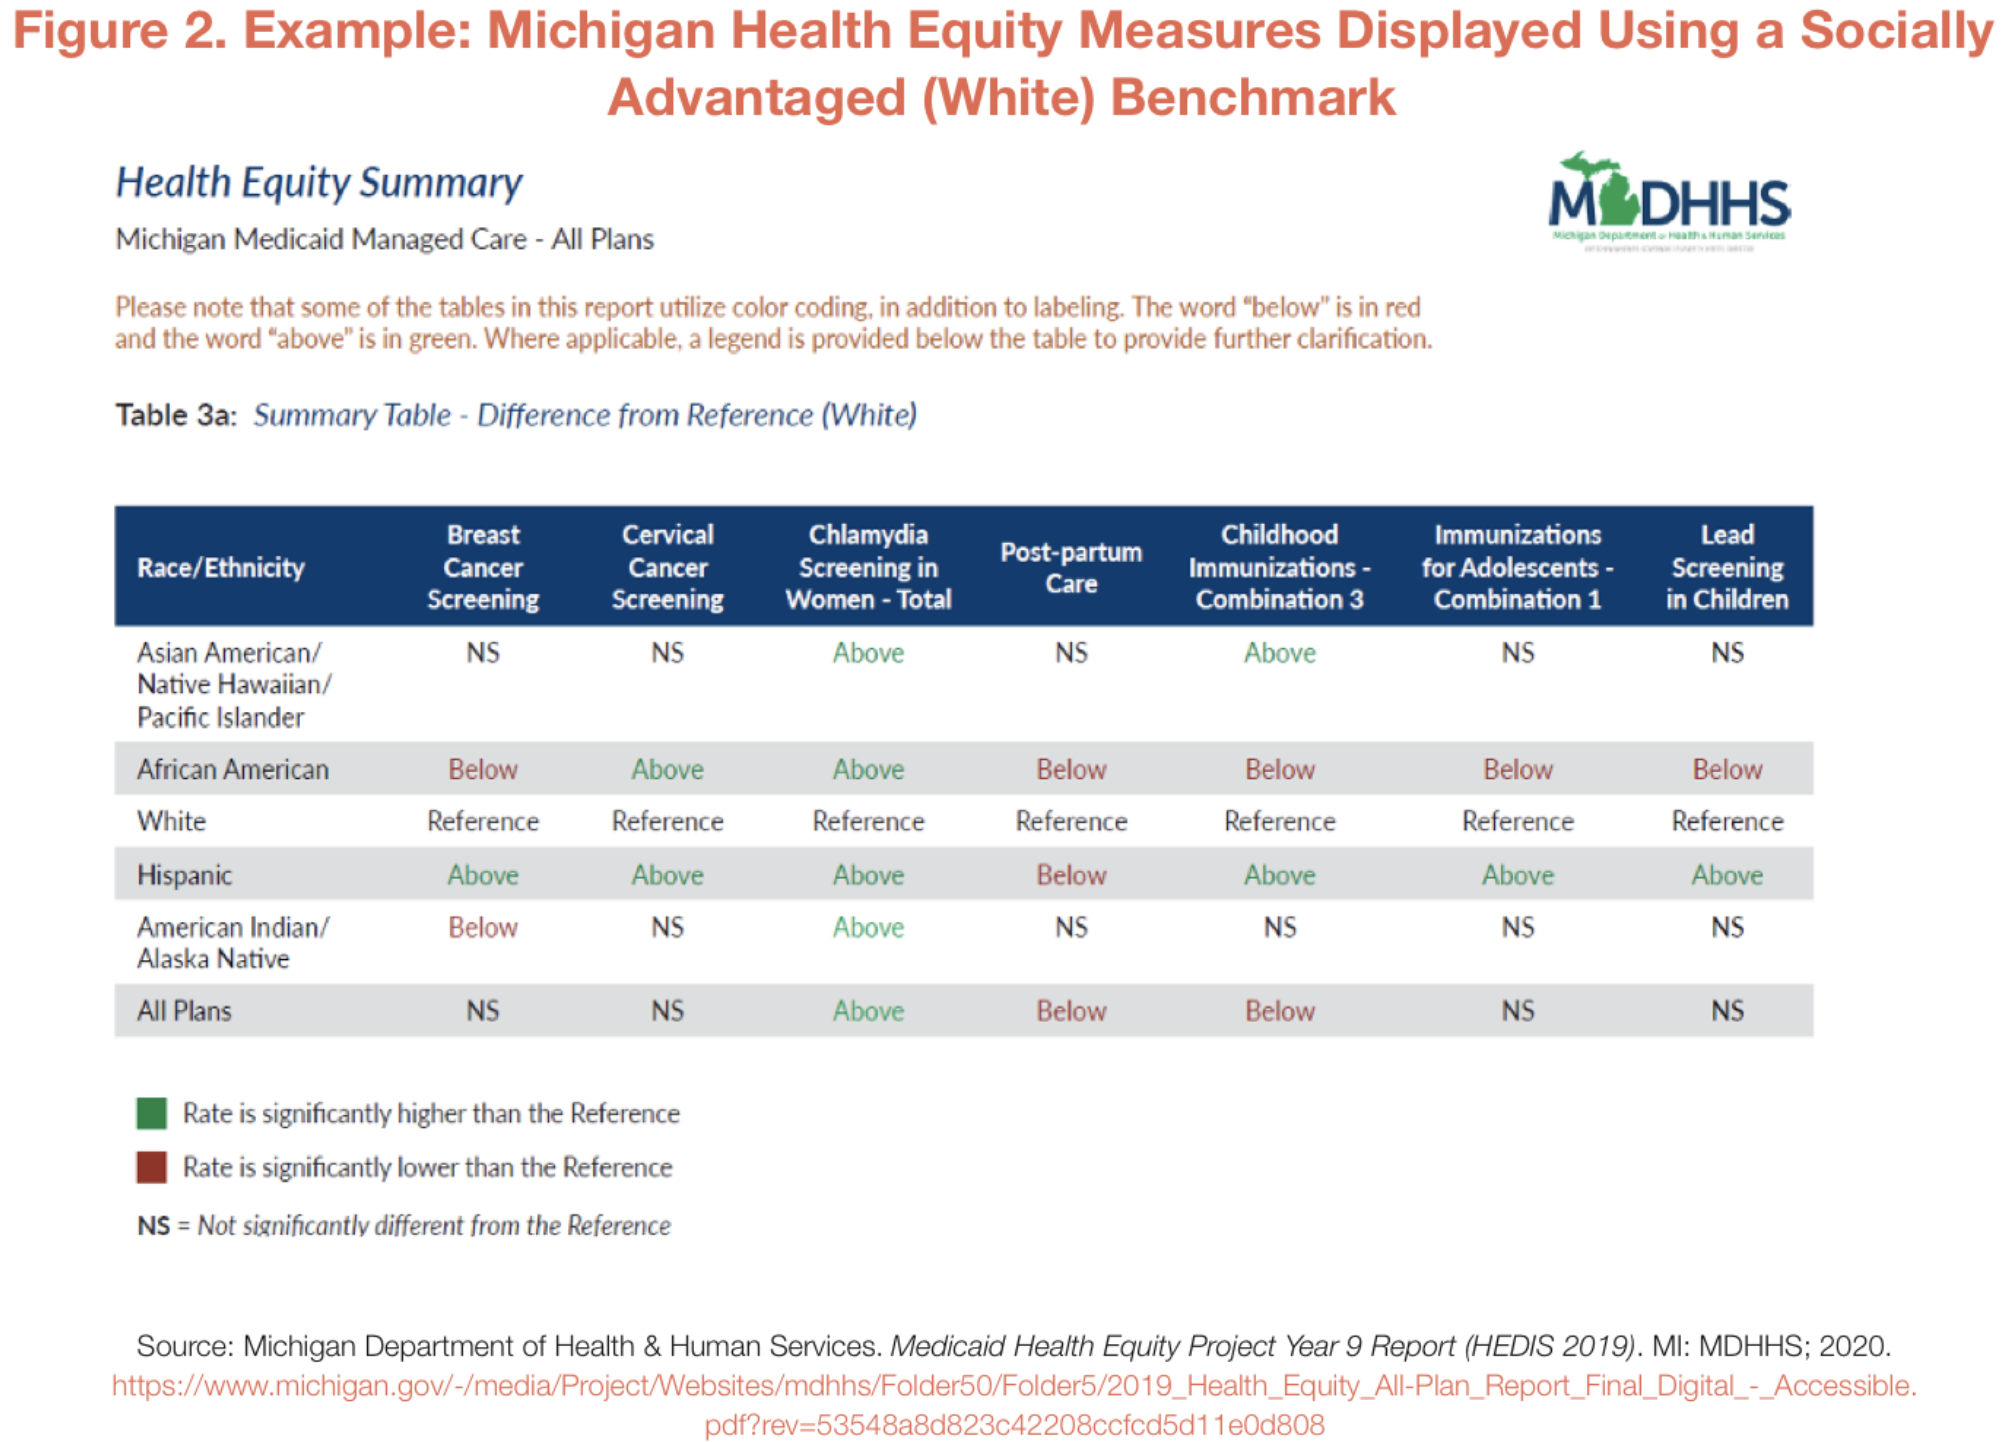
\includegraphics[width=1\textwidth]{fig11.png}
\end{figure}
\begin{figure}[H]
    \centering
    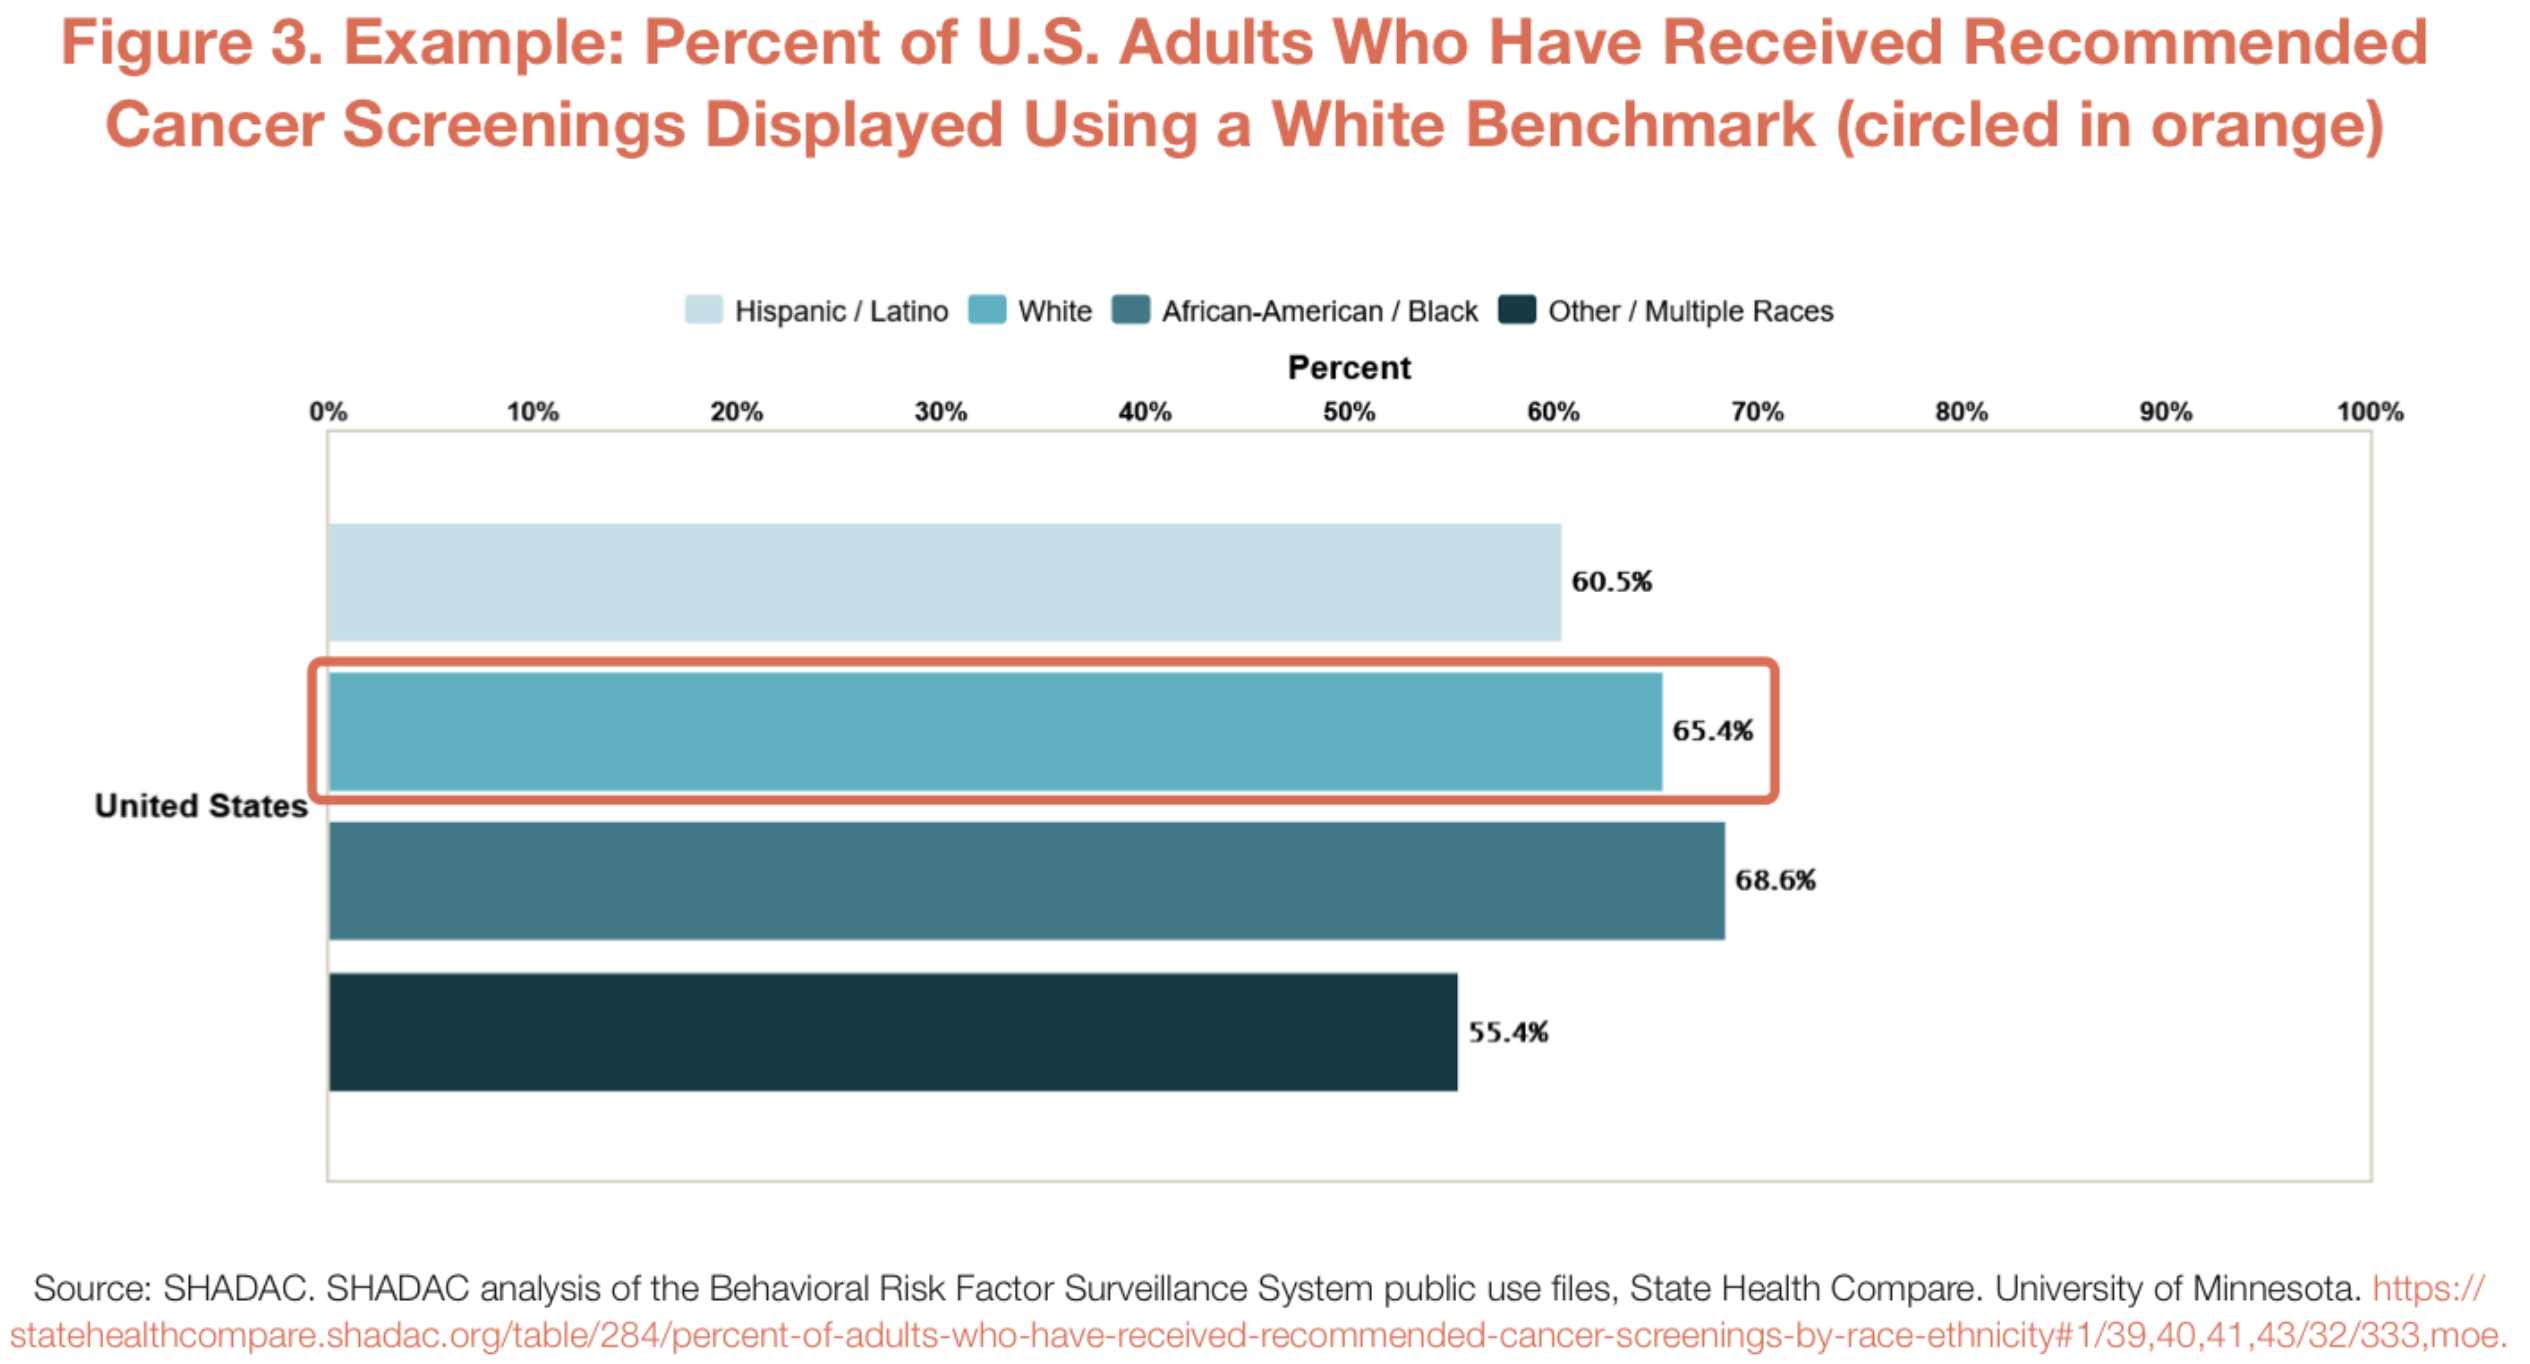
\includegraphics[width=1\textwidth]{fig12.png}
\end{figure}
\begin{figure}[H]
    \centering
    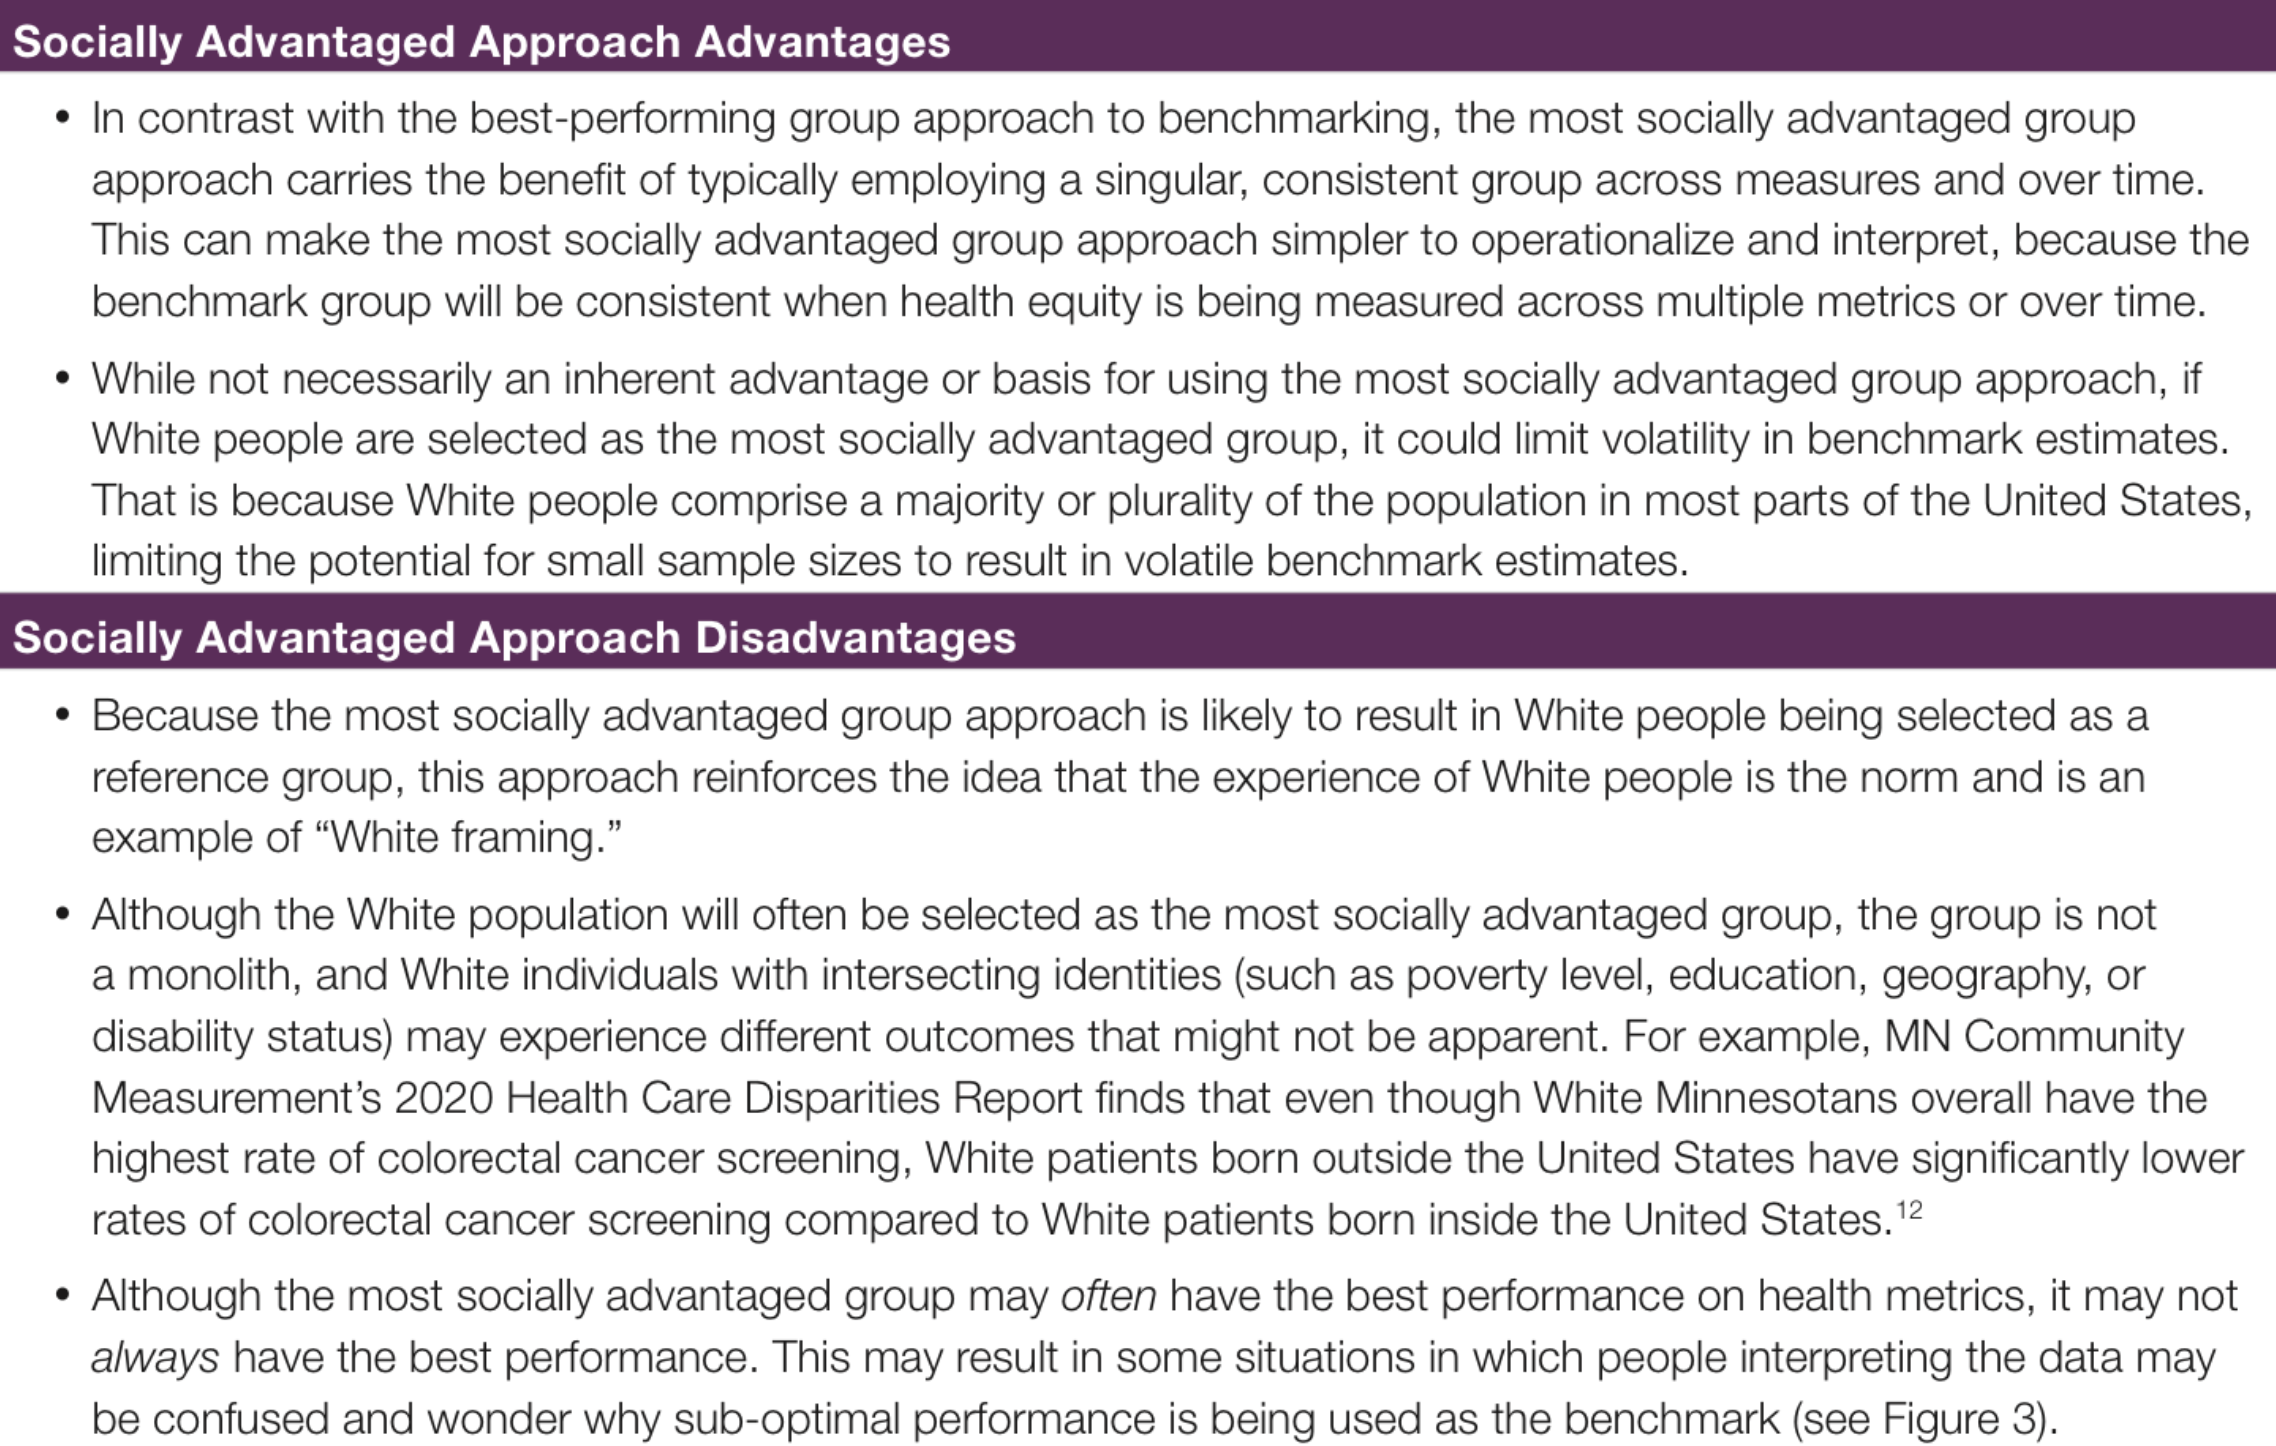
\includegraphics[width=1\textwidth]{fig13.png}
\end{figure}
\begin{figure}[H]
    \centering
    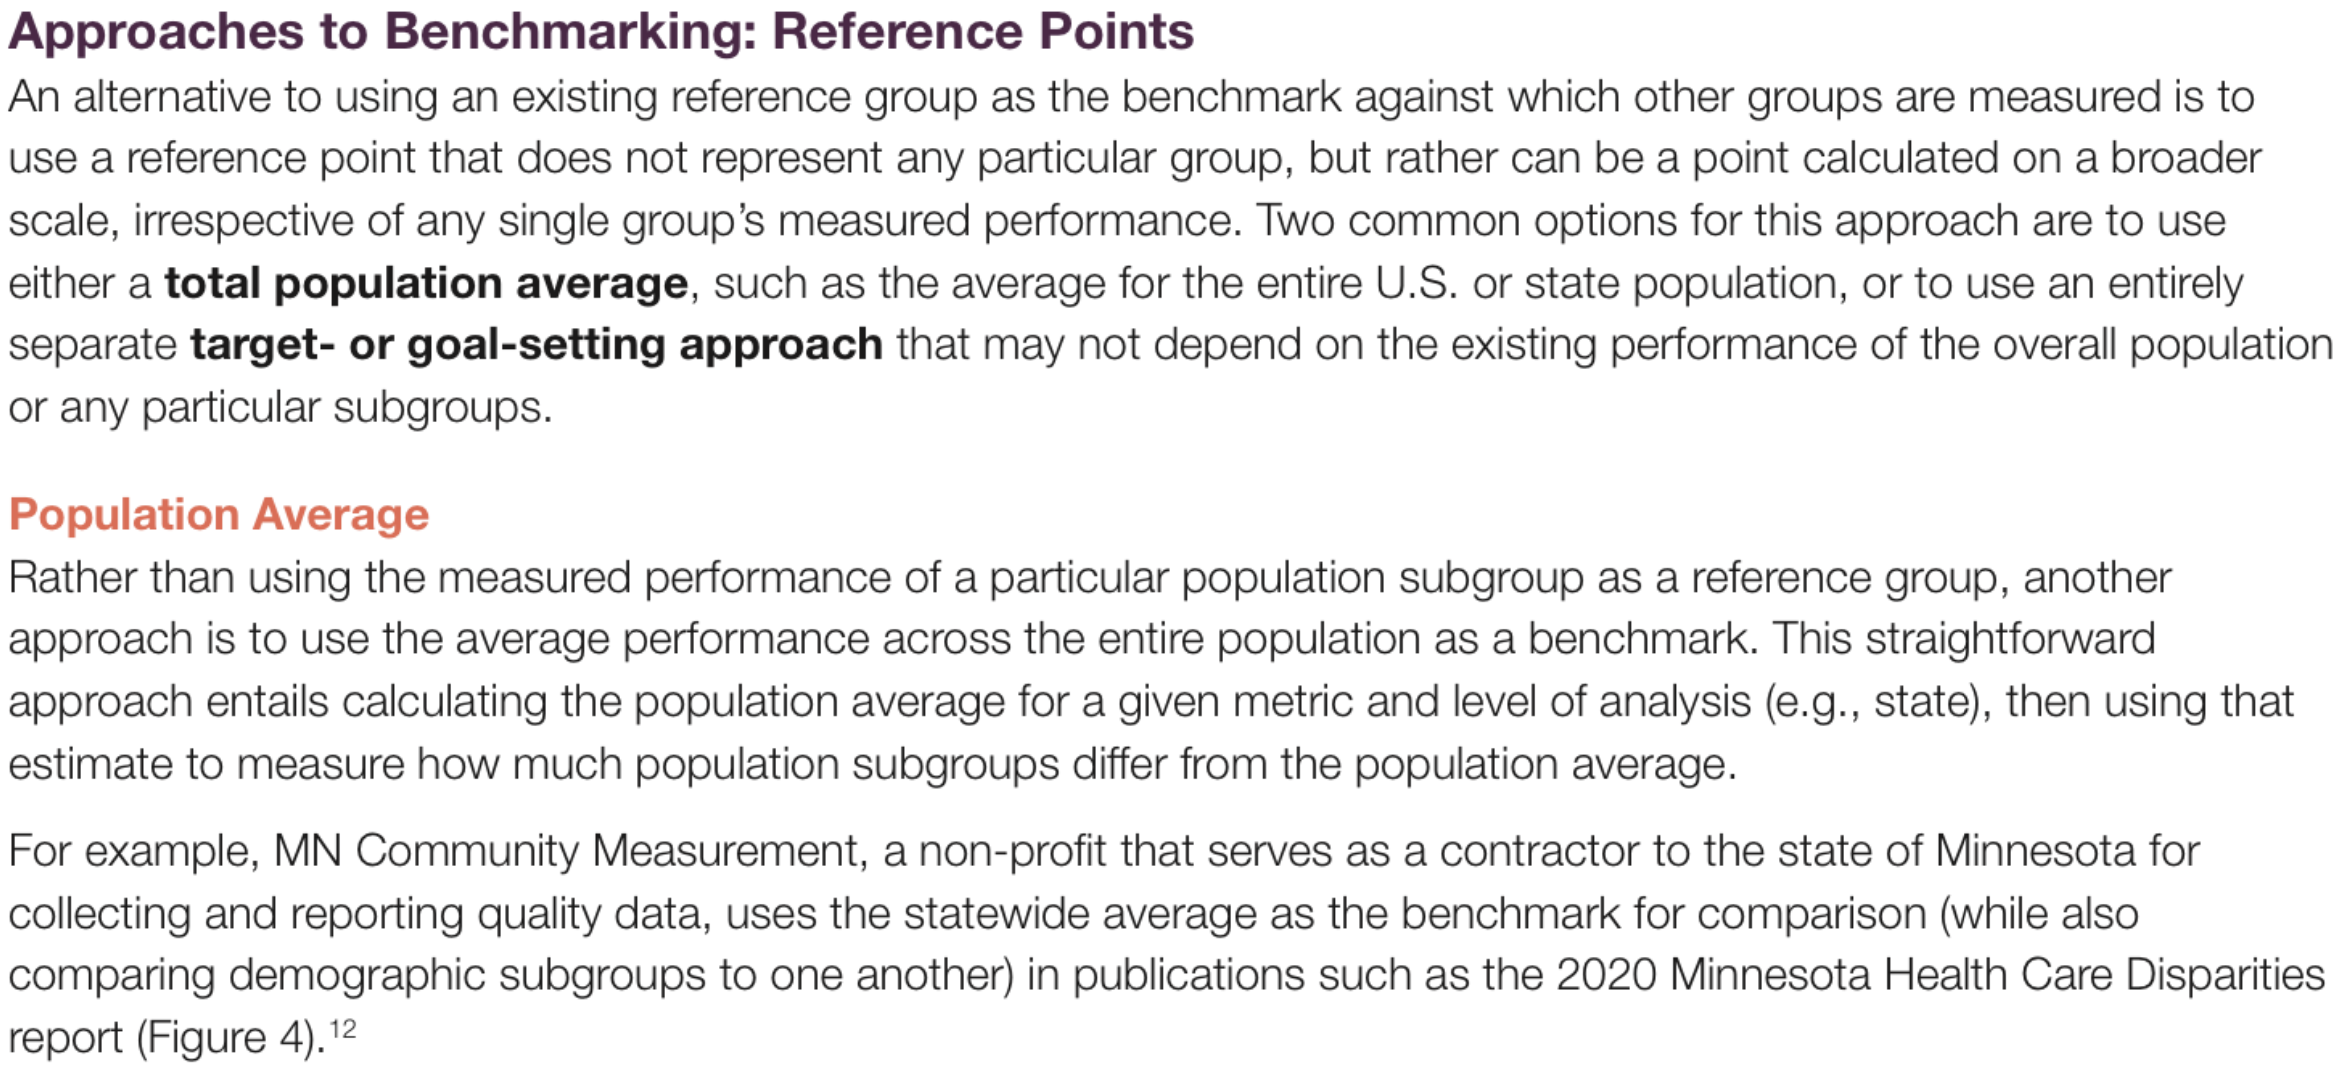
\includegraphics[width=1\textwidth]{fig14.png}
\end{figure}
\begin{figure}[H]
    \centering
    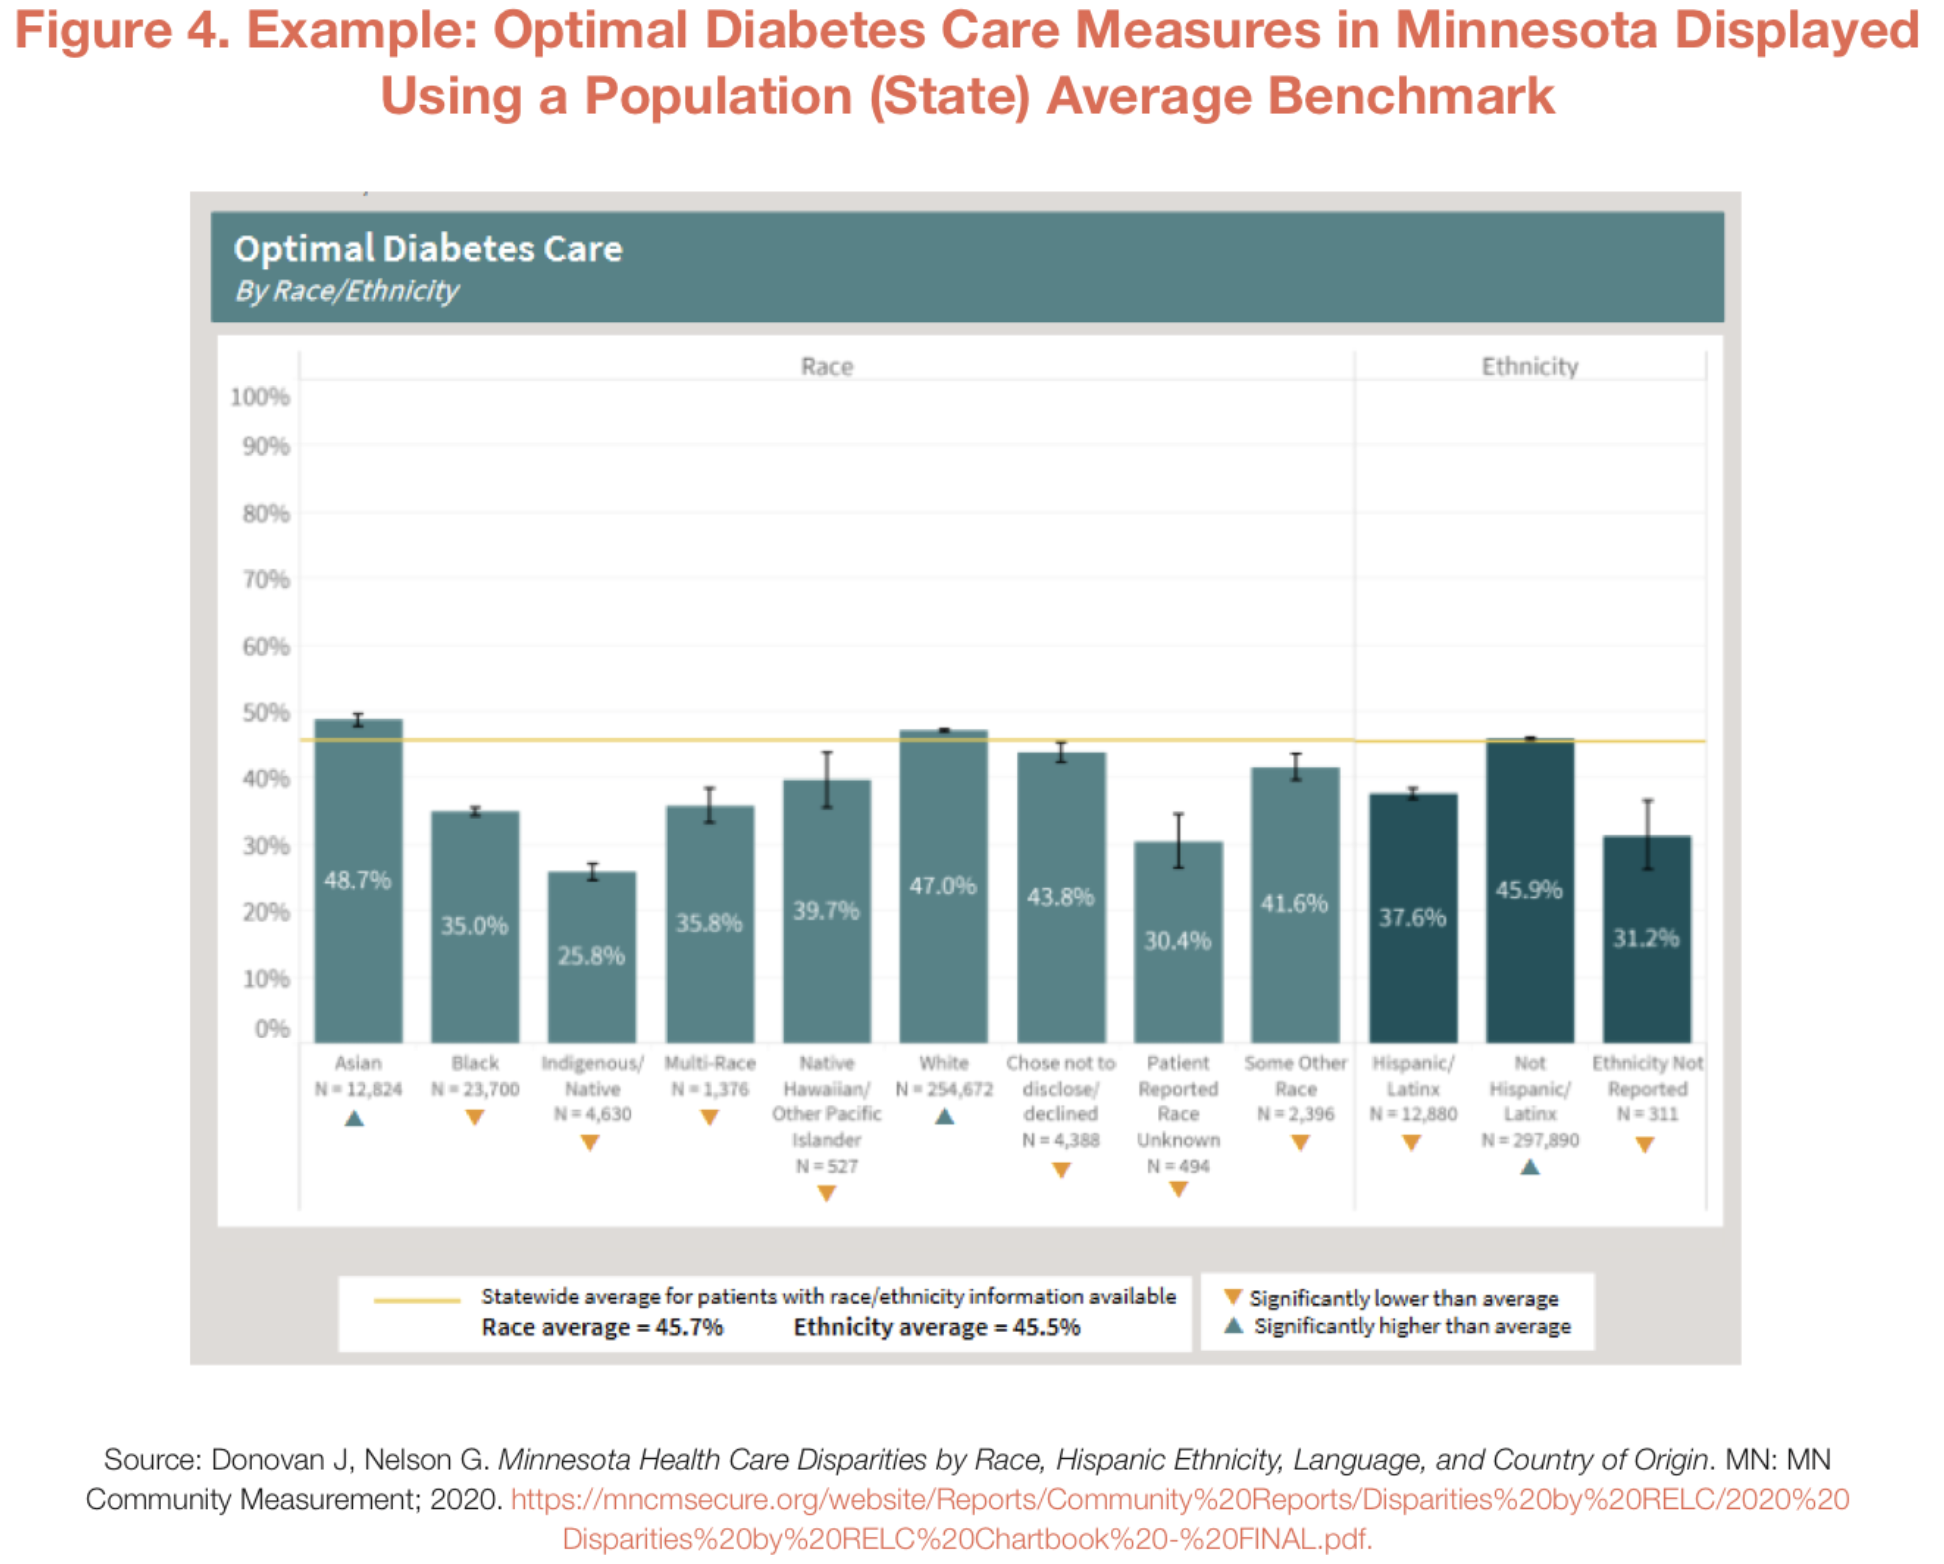
\includegraphics[width=1\textwidth]{fig15.png}
\end{figure}
\newpage
\begin{figure}[H]
    \centering
    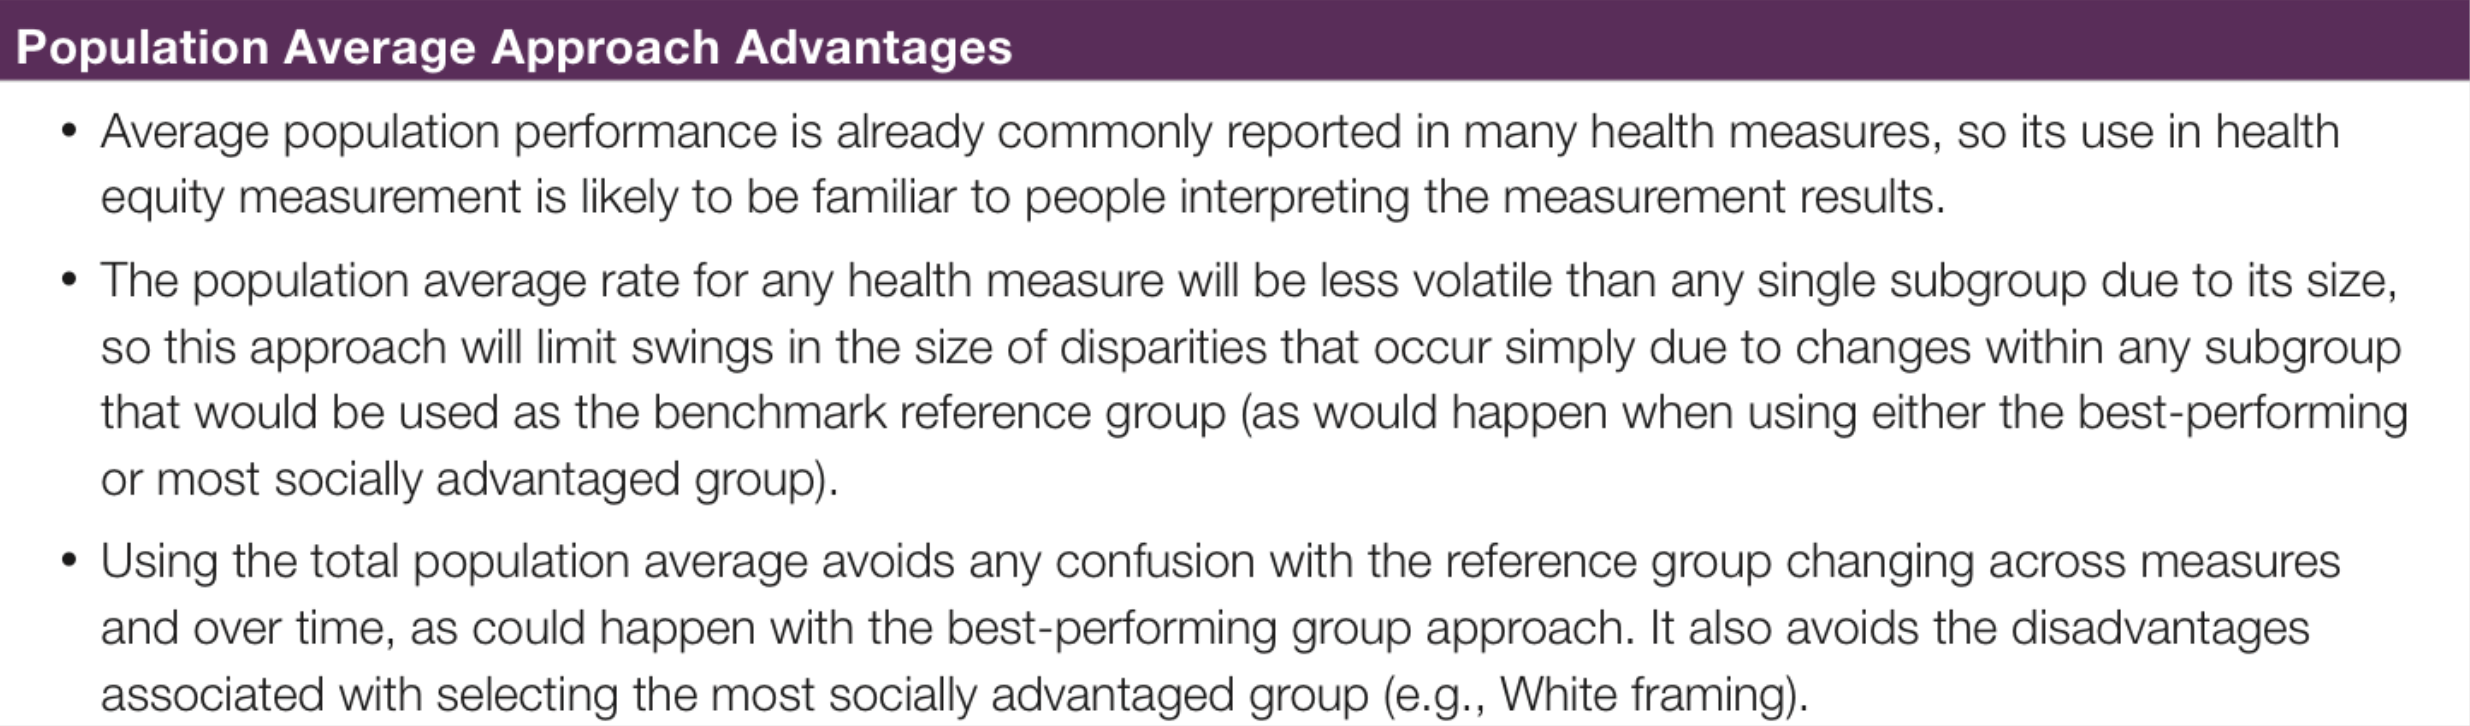
\includegraphics[width=1\textwidth]{fig16.png}
\end{figure}
\begin{figure}[H]
    \centering
    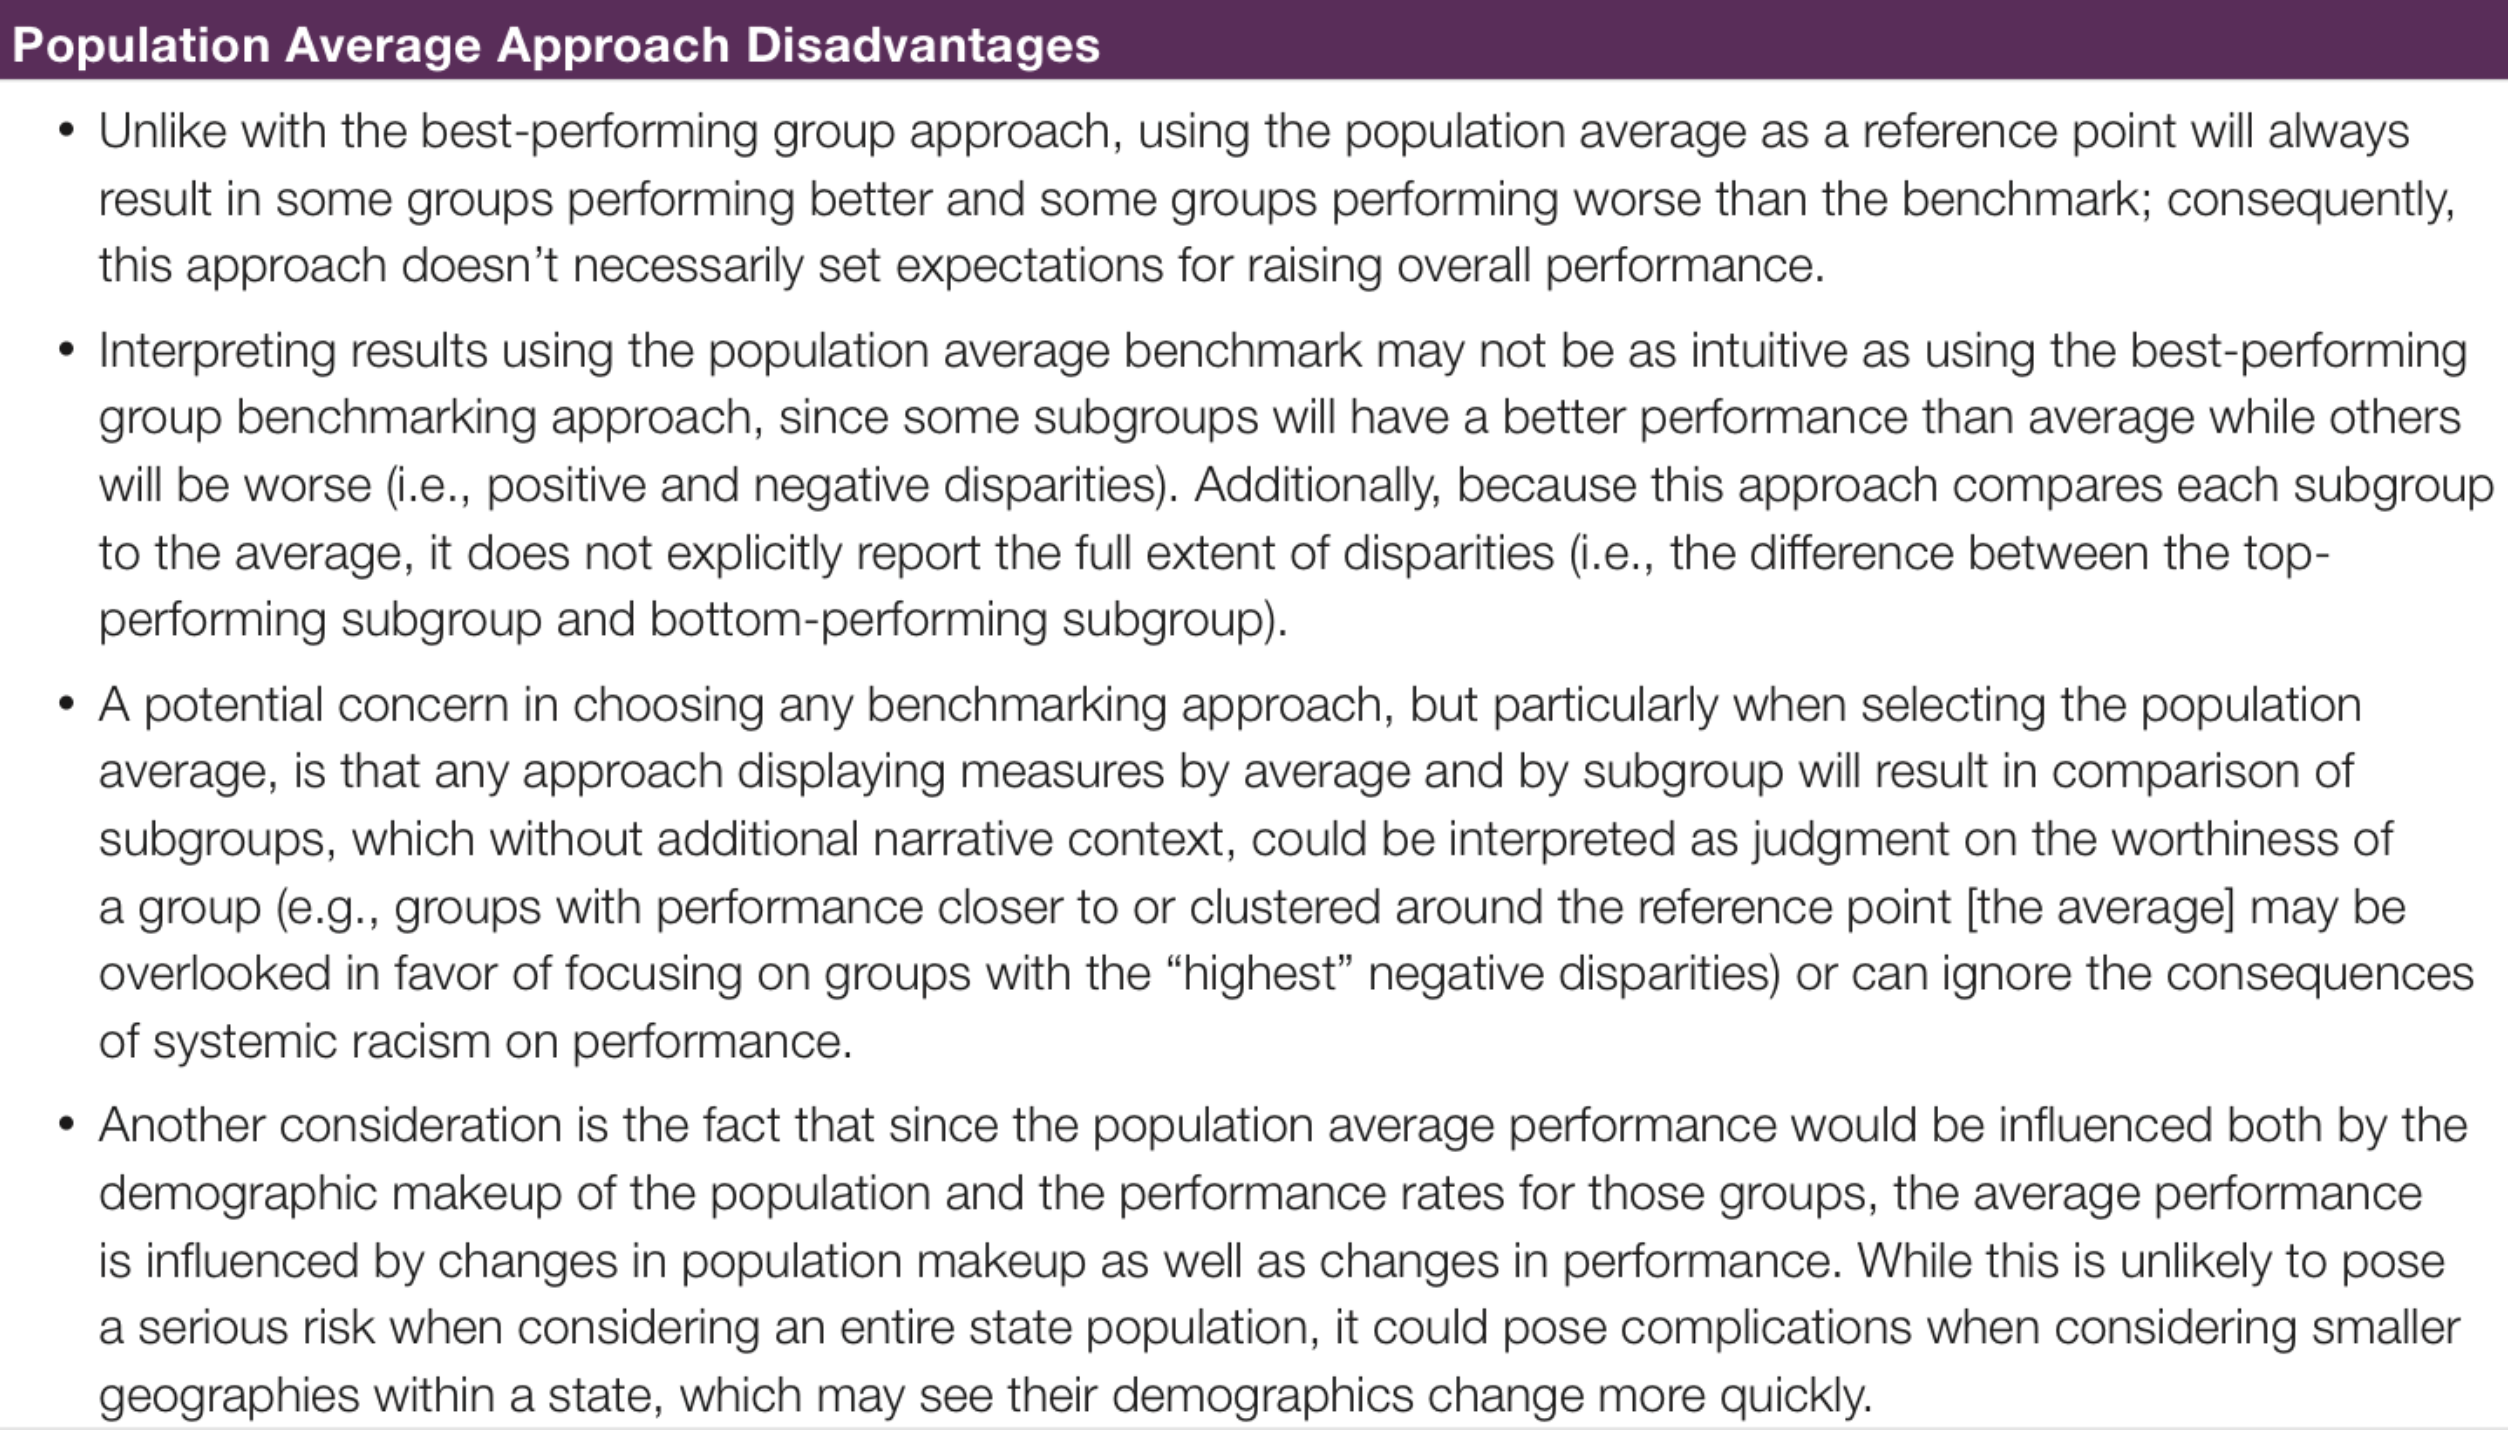
\includegraphics[width=1\textwidth]{fig17.png}
\end{figure}
\begin{figure}[H]
    \centering
    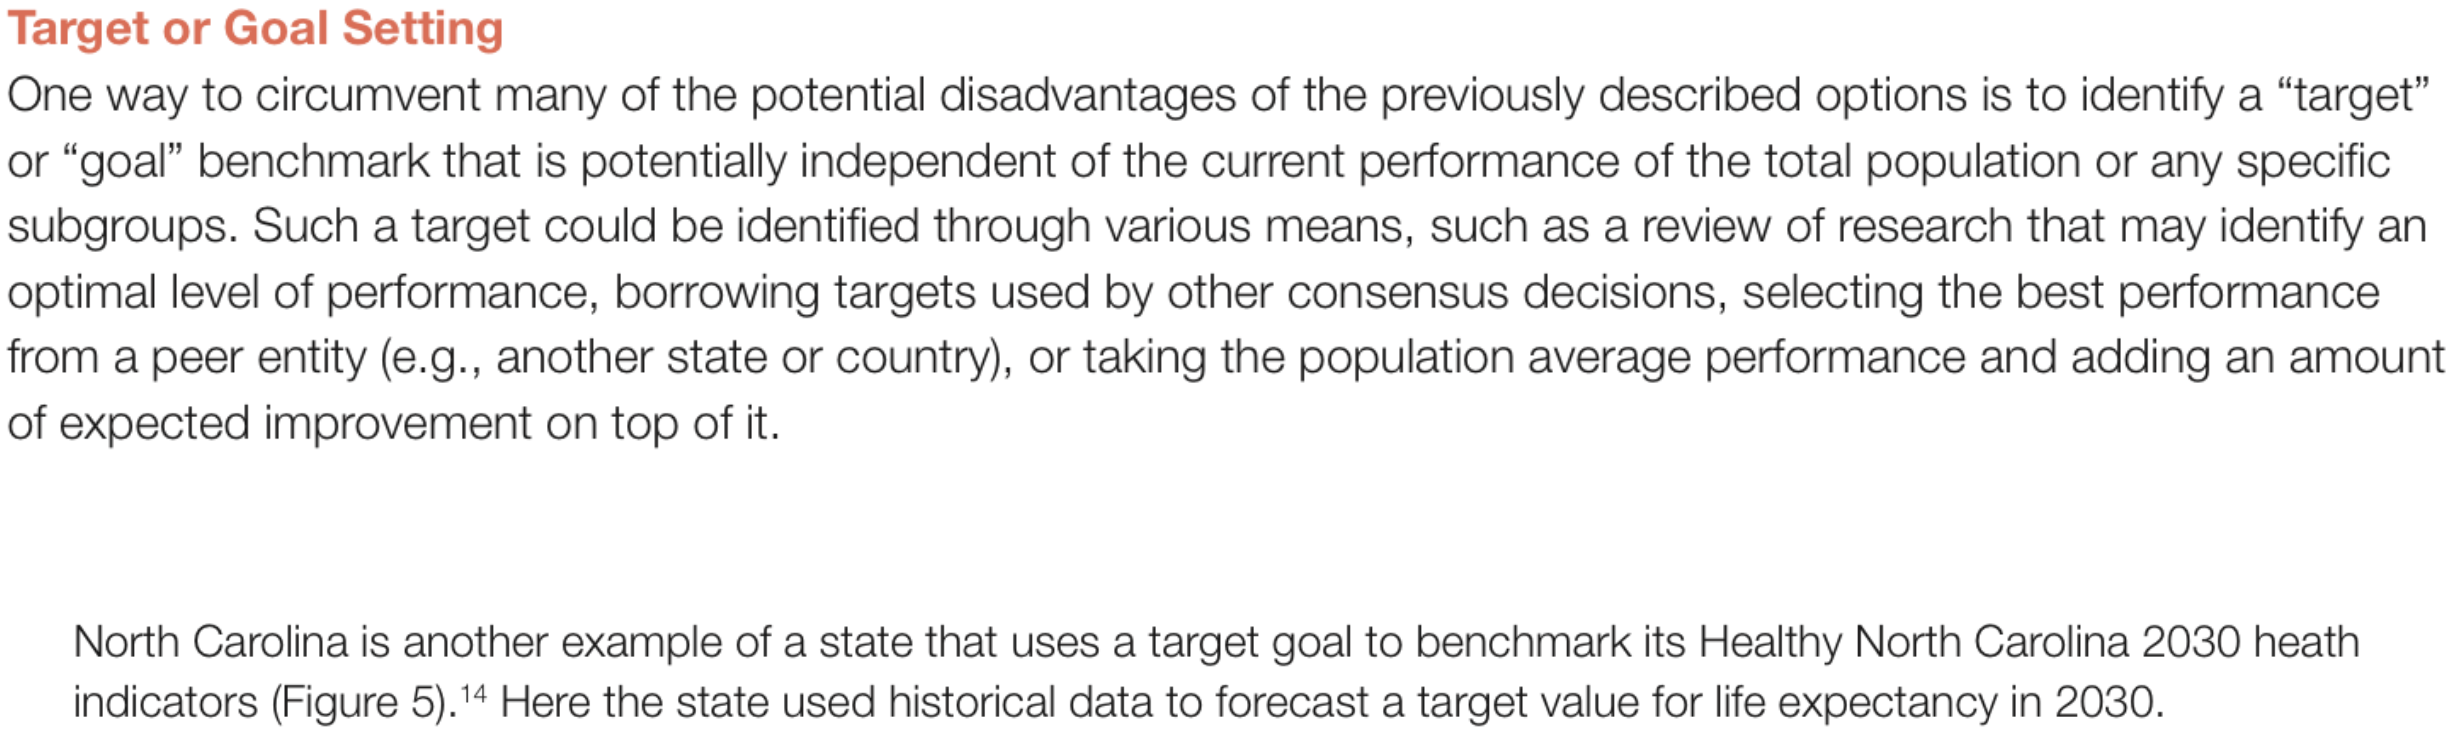
\includegraphics[width=1\textwidth]{fig18.png}
\end{figure}
\begin{figure}[H]
    \centering
    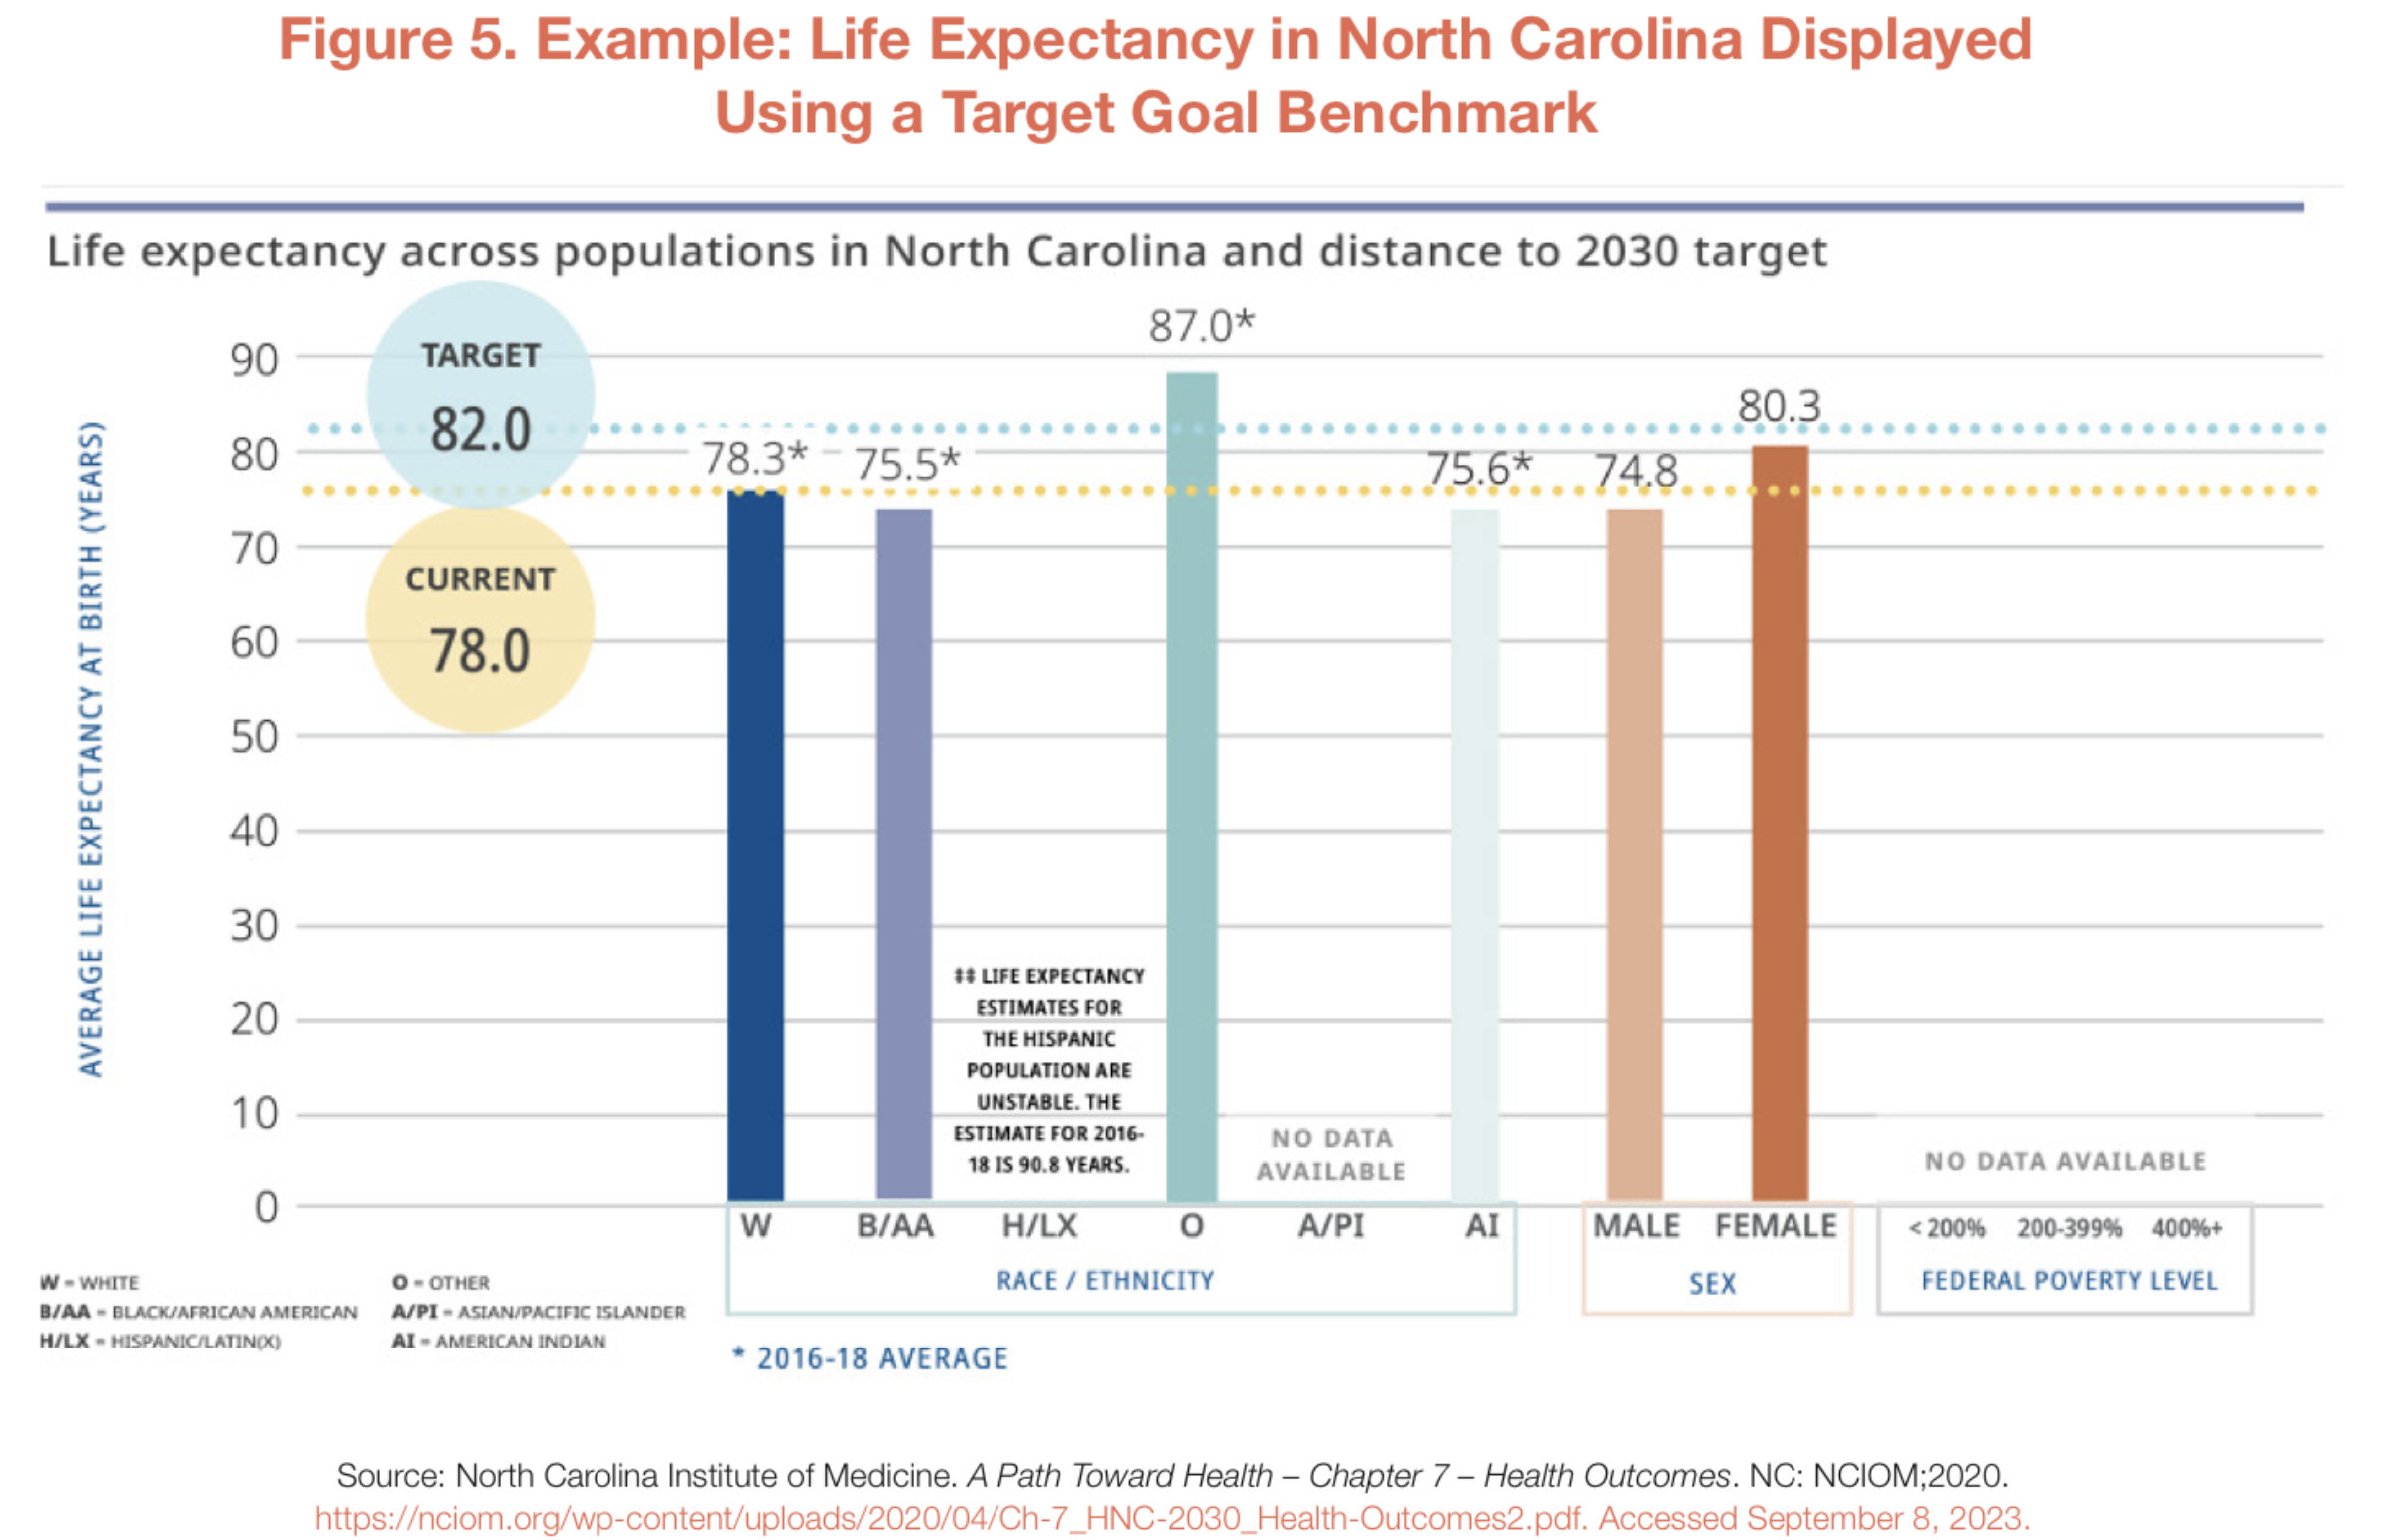
\includegraphics[width=1\textwidth]{fig19.png}
\end{figure}
\begin{figure}[H]
    \centering
    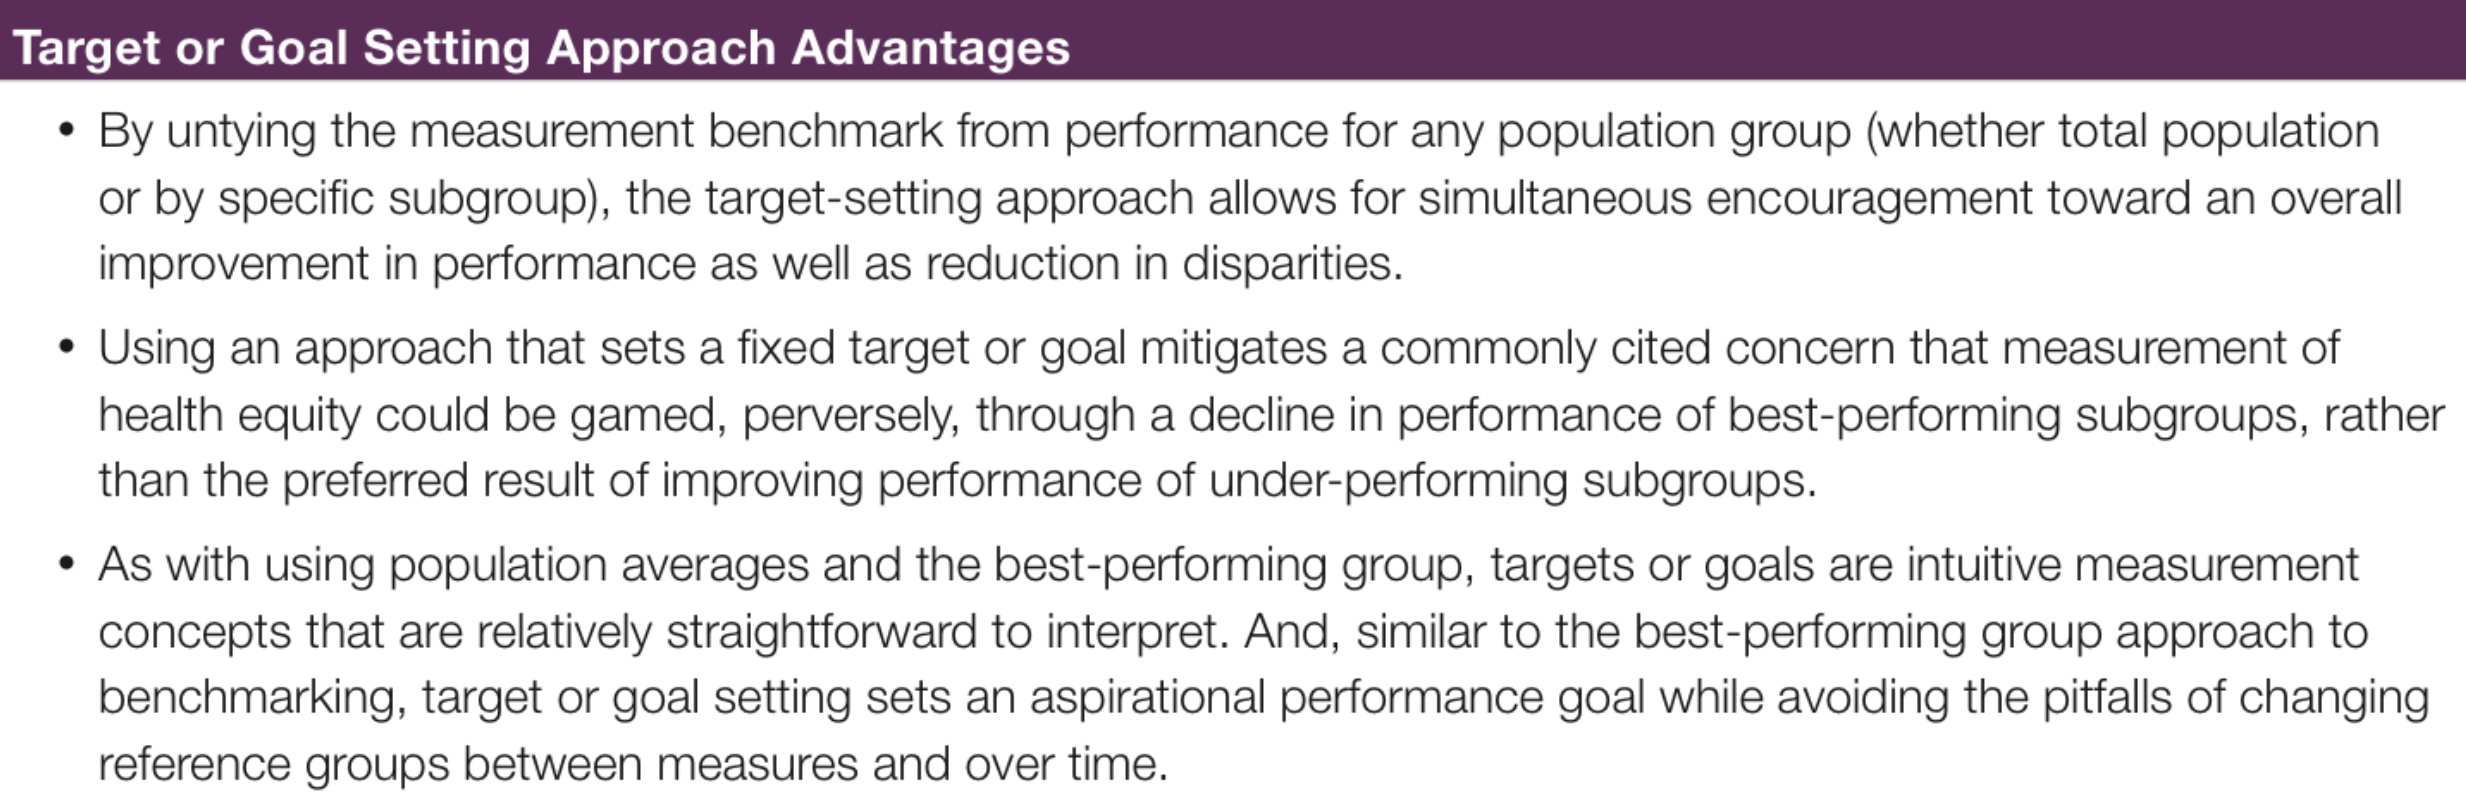
\includegraphics[width=1\textwidth]{fig20.png}
\end{figure}
\begin{figure}[H]
    \centering
    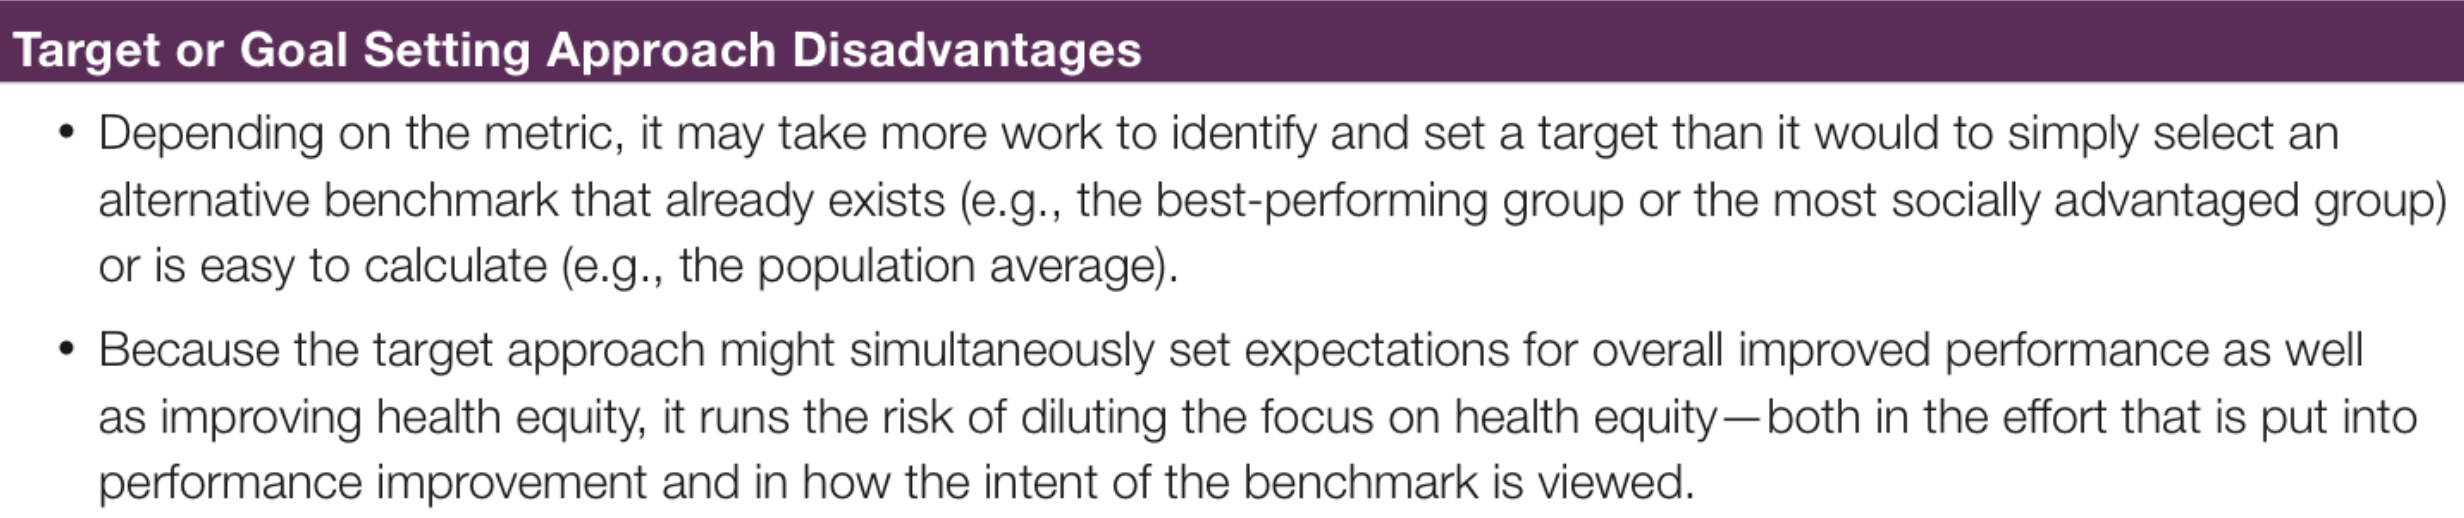
\includegraphics[width=1\textwidth]{fig21.png}
\end{figure}

\subsection*{Adding a Continuous Predictor to Model (ANCOVA)}

- Suppose we add \textcolor{blue}{log(ppgdp)} to the model.
\begin{figure}[H]
    \centering
    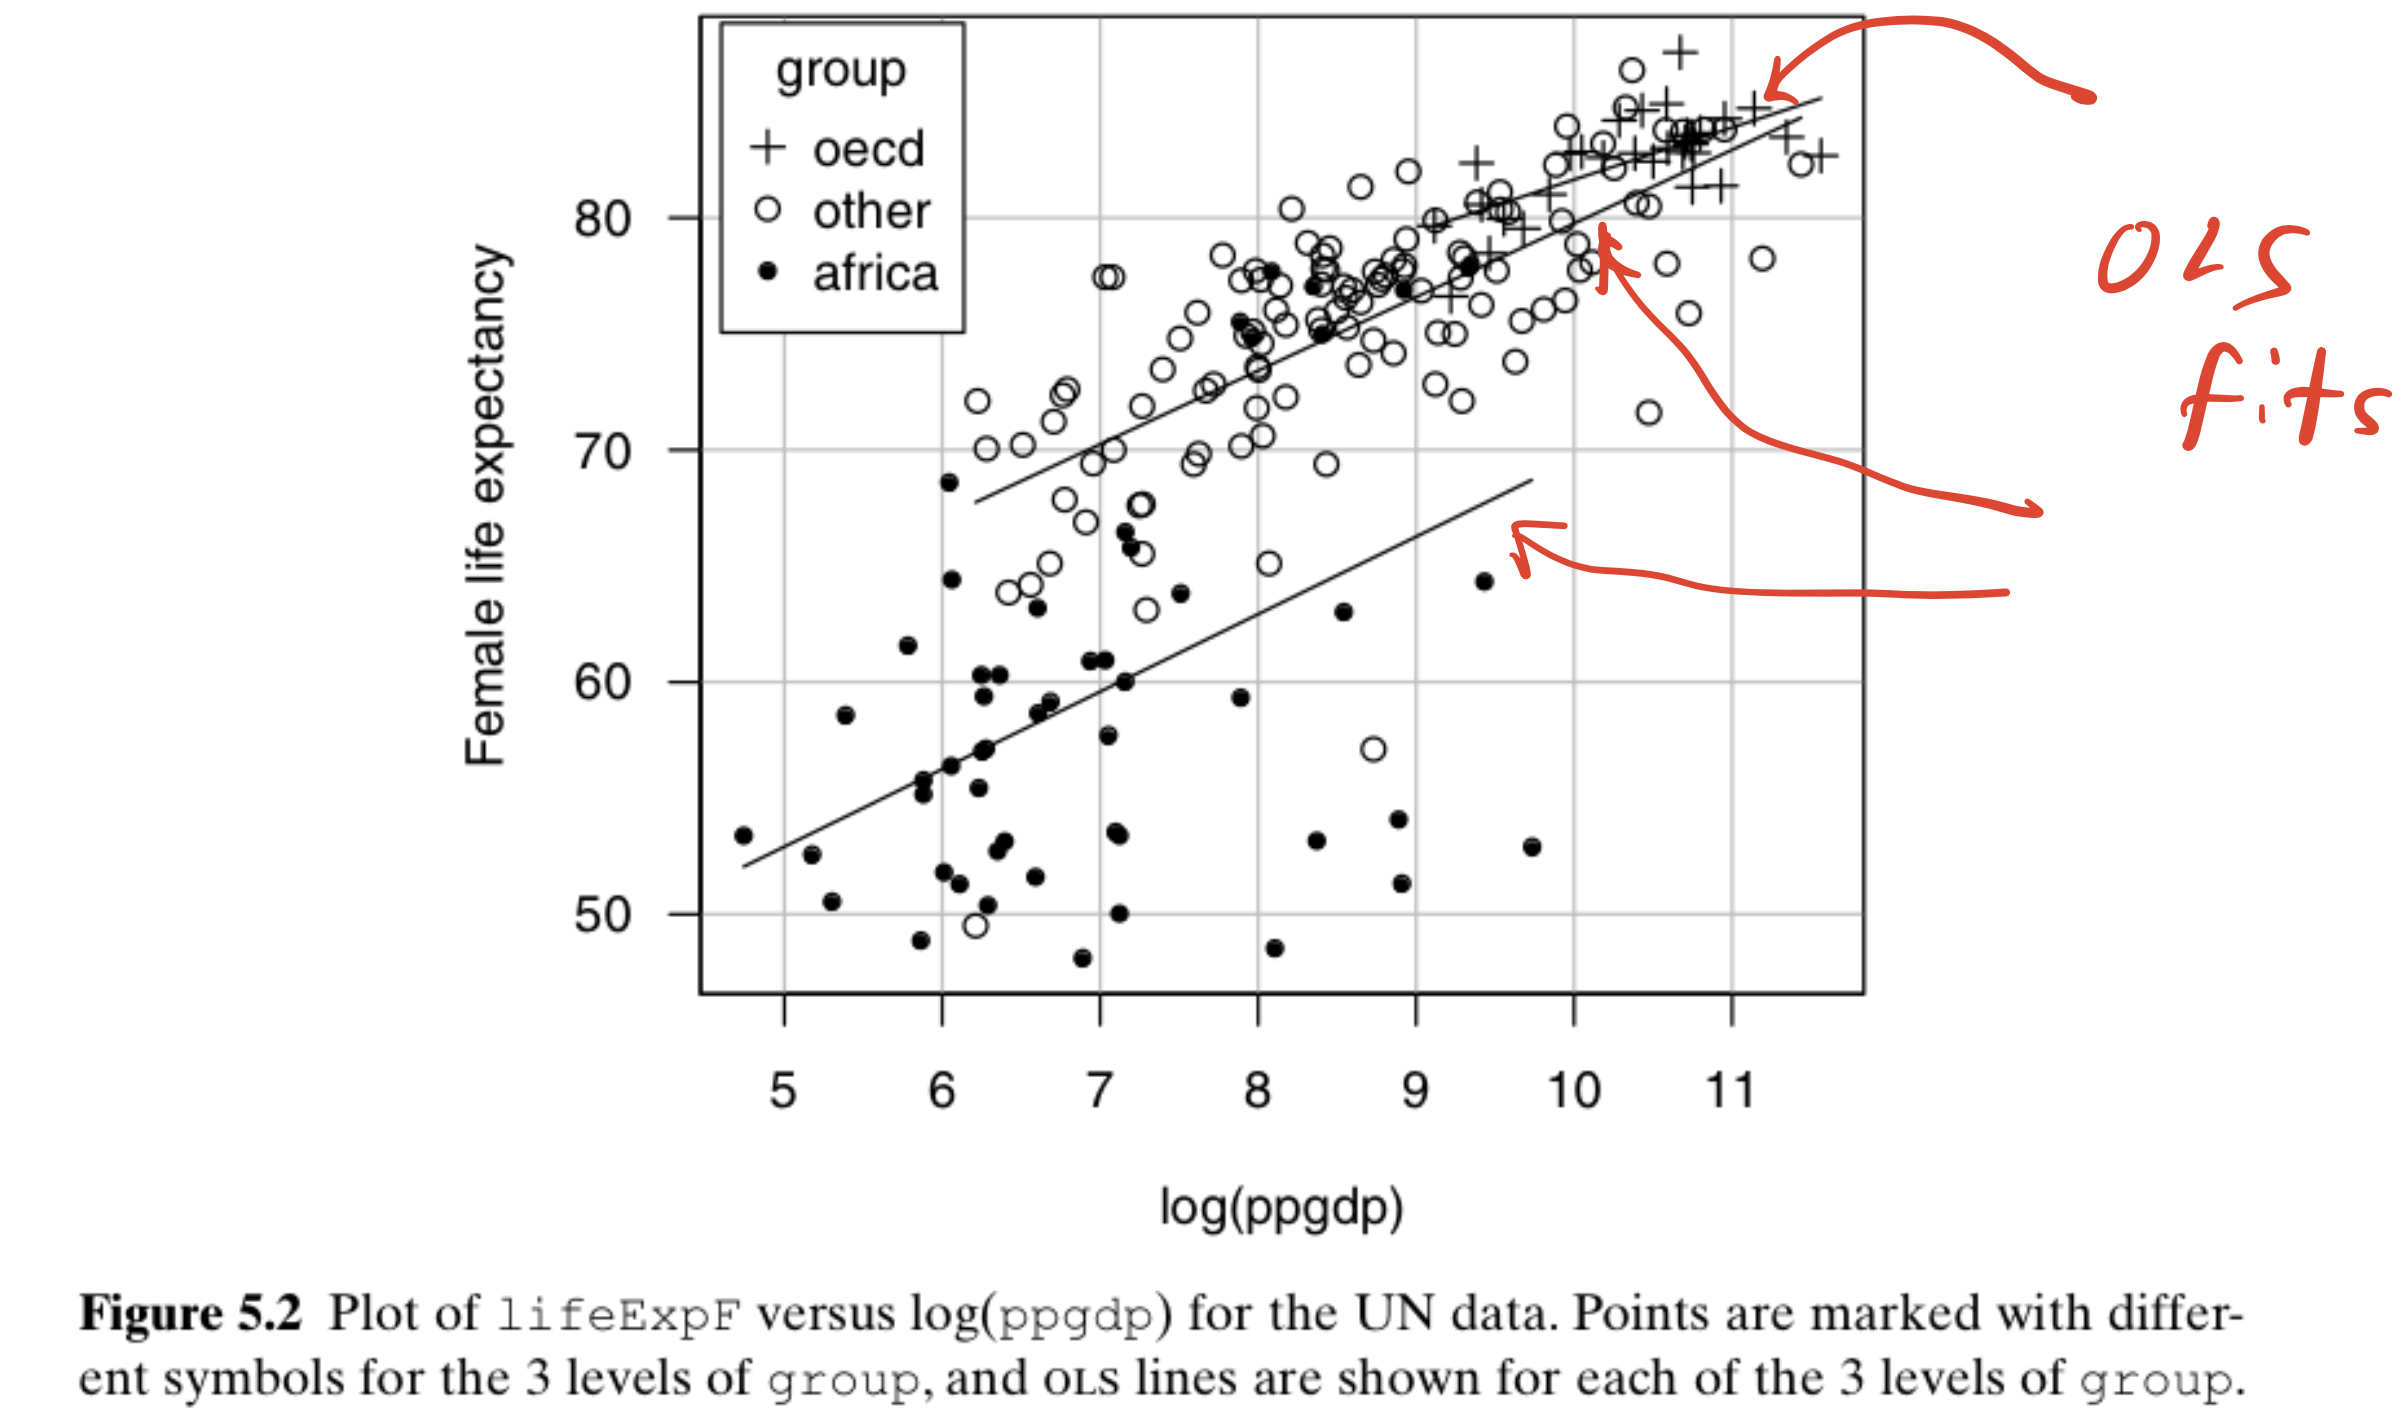
\includegraphics[width=1\textwidth]{fig22.png}
\end{figure}
\noindent
Can write this out as for $group = j$:
\[
E(\textcolor{blue}{\text{lifeExp}} \mid \log(\textcolor{blue}{\text{ppgdp}}) = x, \, \text{group} = j) = \zeta_{0j} + \zeta_{1j} x
\quad (j = 1, \dots, d)
\]
\[
\Rightarrow 2d = 6 \text{ parameters } \quad \text{(separate slopes and intercepts)}
\]
Can parametrize differently as:
\[
E(\textcolor{blue}{\text{lifeExp}} \mid \log(\textcolor{blue}{\text{ppgdp}}) = x, \text{group}) = \beta_0 + \beta_{02} U_2 + \beta_{03} U_3 + \beta_1 x + \beta_{12} U_2 x + \beta_{13} U_3 x
\]
So,
\[
\zeta_{01} = \beta_0 \quad \quad \zeta_{11} = \beta_1 \quad \textcolor{red}{\text{(baseline)}}
\]
\[
\zeta_{02} = \beta_0 + \beta_{02} \quad \quad \zeta_{12} = \beta_1 + \beta_{12}
\]
\[
\zeta_{03} = \beta_0 + \beta_{03} \quad \quad \zeta_{13} = \beta_1 + \beta_{13}
\]
\begin{figure}[H]
    \centering
    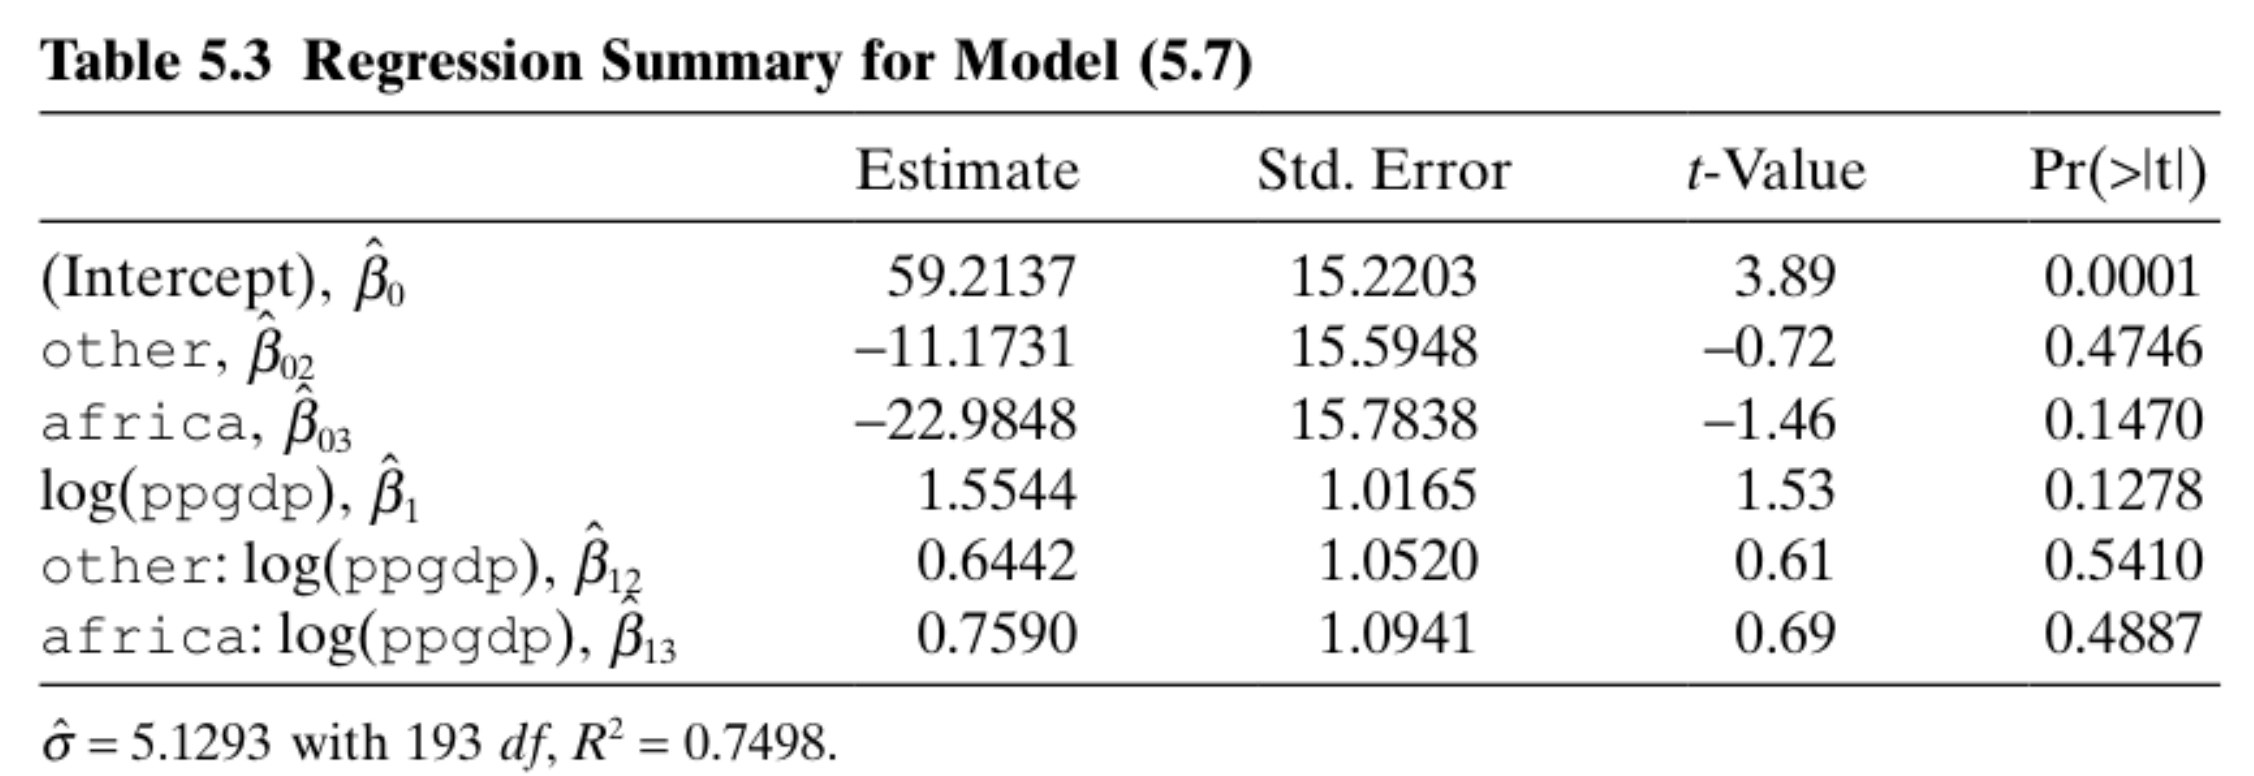
\includegraphics[width=1\textwidth]{fig23.png}
\end{figure}
\begin{figure}[H]
    \centering
    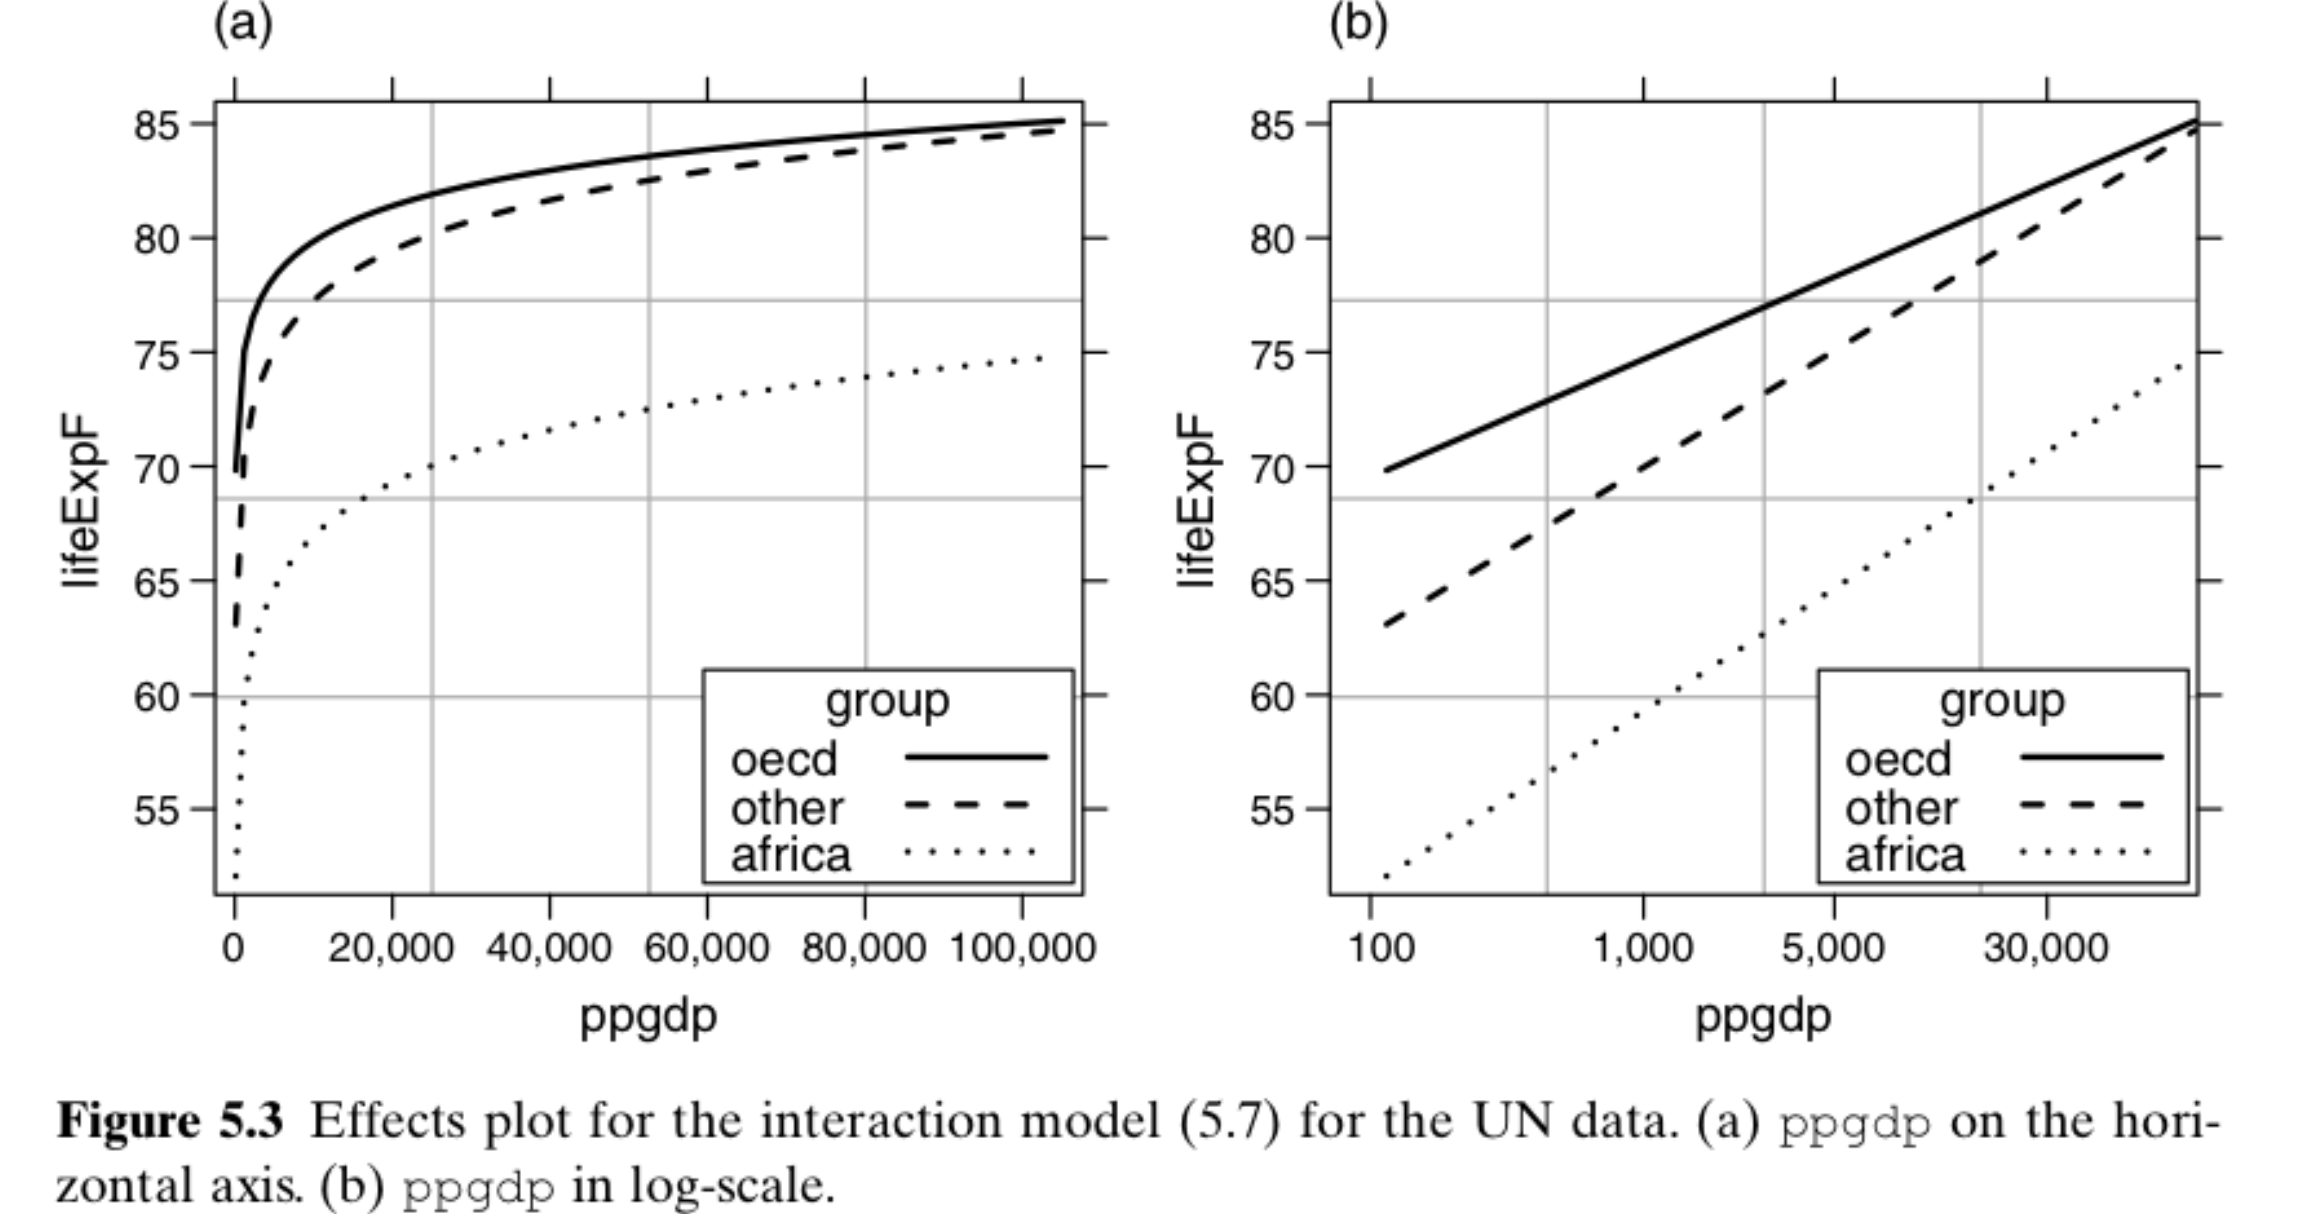
\includegraphics[width=0.95\textwidth]{fig24.png}
\end{figure}
\noindent
\textbf{Case Study: Lead Exposure and Neuro-Psychological Function}\\
\textbf{Task:} examine association between lead exposure and developmental features in children.\\
\textbf{Study:} Done in El Paso, TX\\
    Control group ($n = 78$)\\
    - blood-lead levels $< 40 \, \text{mg/100ml}$ in both 1972 and 1973\\
    Exposed group ($n = 46$)\\
     - blood-lead levels $\geq 40 \, \text{mg/100ml}$ in either 1972 or 1973\\
\textbf{Response:} \# finger wrist taps / 10 seconds in dominant hand\\

\subsection*{Dummy Variable for Two-Level Categorical Predictors}
\begin{itemize}
    \item Categories of predictor: $A, B$ (for example)
    \item First category = reference cell, gets a zero
    \item Second category gets a 1.0
    \item Formal definition of dummy variable: $x = I[\text{category} = B]$, \\$I[w] = 1$ if $w$ is true, 0 otherwise
    \item $\alpha + \beta x = \alpha + \beta I[\text{category} = B] =$\\
        $\alpha$ for category $A$ subjects\\
        $\alpha + \beta$ for category $B$ subjects\\
        $\beta =$ mean difference $(B - A)$
\end{itemize}

\subsection*{Two-Sample \textit{t}-test vs. Simple Linear Regression}

\begin{itemize}
    \item They are equivalent in every sense:
    \begin{itemize}
        \item $P$-value
        \item Estimates and C.L.s after rephrasing the model
        \item Assumptions (equal variance assumption of two groups in \textit{t}-test is the same as constant variance of $Y|X$ for every $X$)
    \end{itemize}
\end{itemize}
\[
\hat{\alpha} = \bar{y}_A
\]

\[
\hat{\beta} = \bar{y}_B - \bar{y}_A
\]

\[
SE(\hat{\beta}) = SE\left( \bar{Y}_B - \bar{Y}_A \right)
\]

\section*{Analysis of Covariance}

\begin{itemize}
    \item Multiple regression can extend the \textit{t}-test
    \begin{itemize}
        \item More than 2 groups (multiple dummy variables can do multiple-group ANOVA)
        \item Allow for categorical or continuous adjustment variables (covariates, co-variables)
    \end{itemize}

    \item Model: $MAXFWT = \alpha + \beta_1 \text{age} + \beta_2 \text{sex} + e$
    
    \item Rosner coded $sex = 1, 2$ for male, female.
    \begin{itemize}
        \item Does not affect interpretation of $\beta_2$ but makes interpretation of $\alpha$ more tricky (mean $MAXFWT$ when $age = 0$ and $sex = 0$ which is impossible by this coding).
    \end{itemize}
    
    \item Better coding would have been $sex = 0, 1$ for male, female
    \begin{itemize}
        \item $\alpha = $ mean $MAXFWT$ for a zero year-old male
        \item $\beta_1 = $ increase in mean $MAXFWT$ per 1-year increase in $age$
        \item $\beta_2 = $ mean $MAXFWT$ for females minus mean $MAXFWT$ for males, holding $age$ constant
    \end{itemize}
    
    \item Create derived variable that indicates exposure in either year.
    \begin{itemize}
        \item Call the variable \textit{exposure} and use the following formula for its derivation: \\
        \texttt{group != 'blood lead < 40mg/100ml in 1972 \& 1973'}
    \end{itemize}

    \item Model: $MAXFWT = \alpha + \beta_1 \text{exposure} + \beta_2 \text{age} + \beta_3 \text{sex} + e$ \\
    \textit{exposure} = \textbf{TRUE} (1) for exposed, \textbf{FALSE} (0) for unexposed
    \item $\beta_1$ = mean $MAXFWT$ for exposed minus mean for unexposed, holding \textit{age} and \textit{sex} constant
\end{itemize}
\begin{figure}[H]
    \centering
    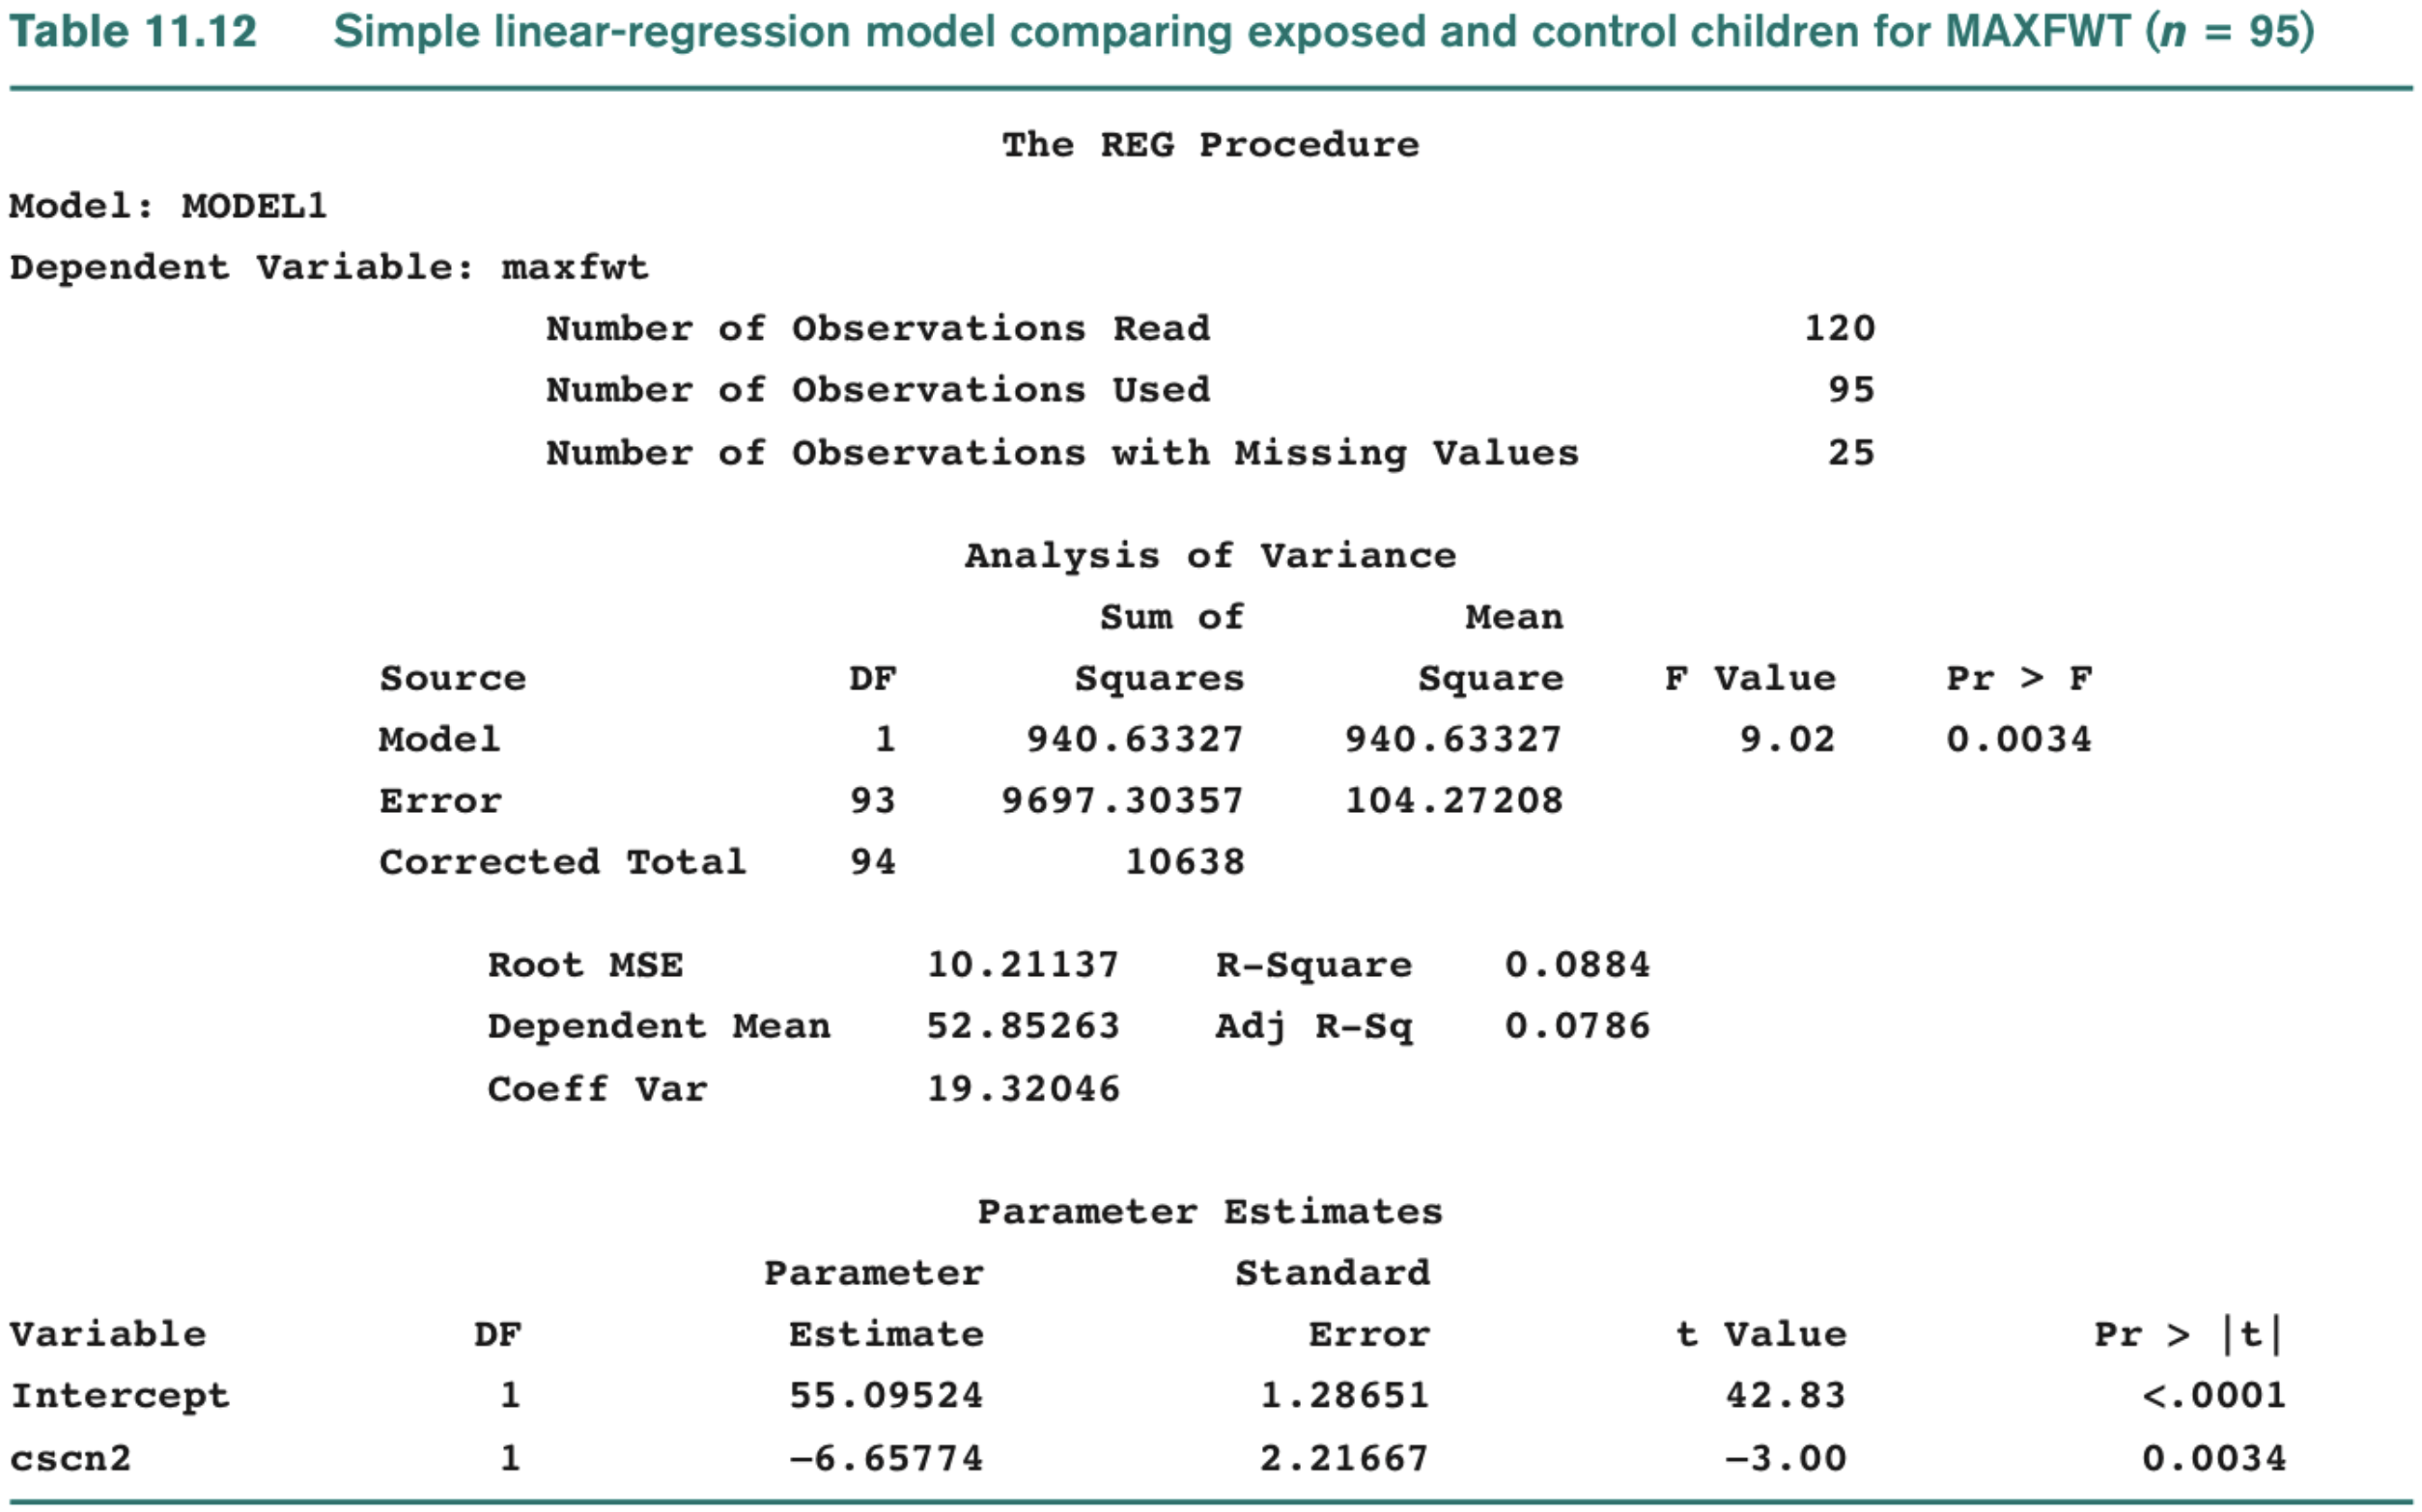
\includegraphics[width=1\textwidth]{fig25.png}
\end{figure}
\begin{figure}[H]
    \centering
    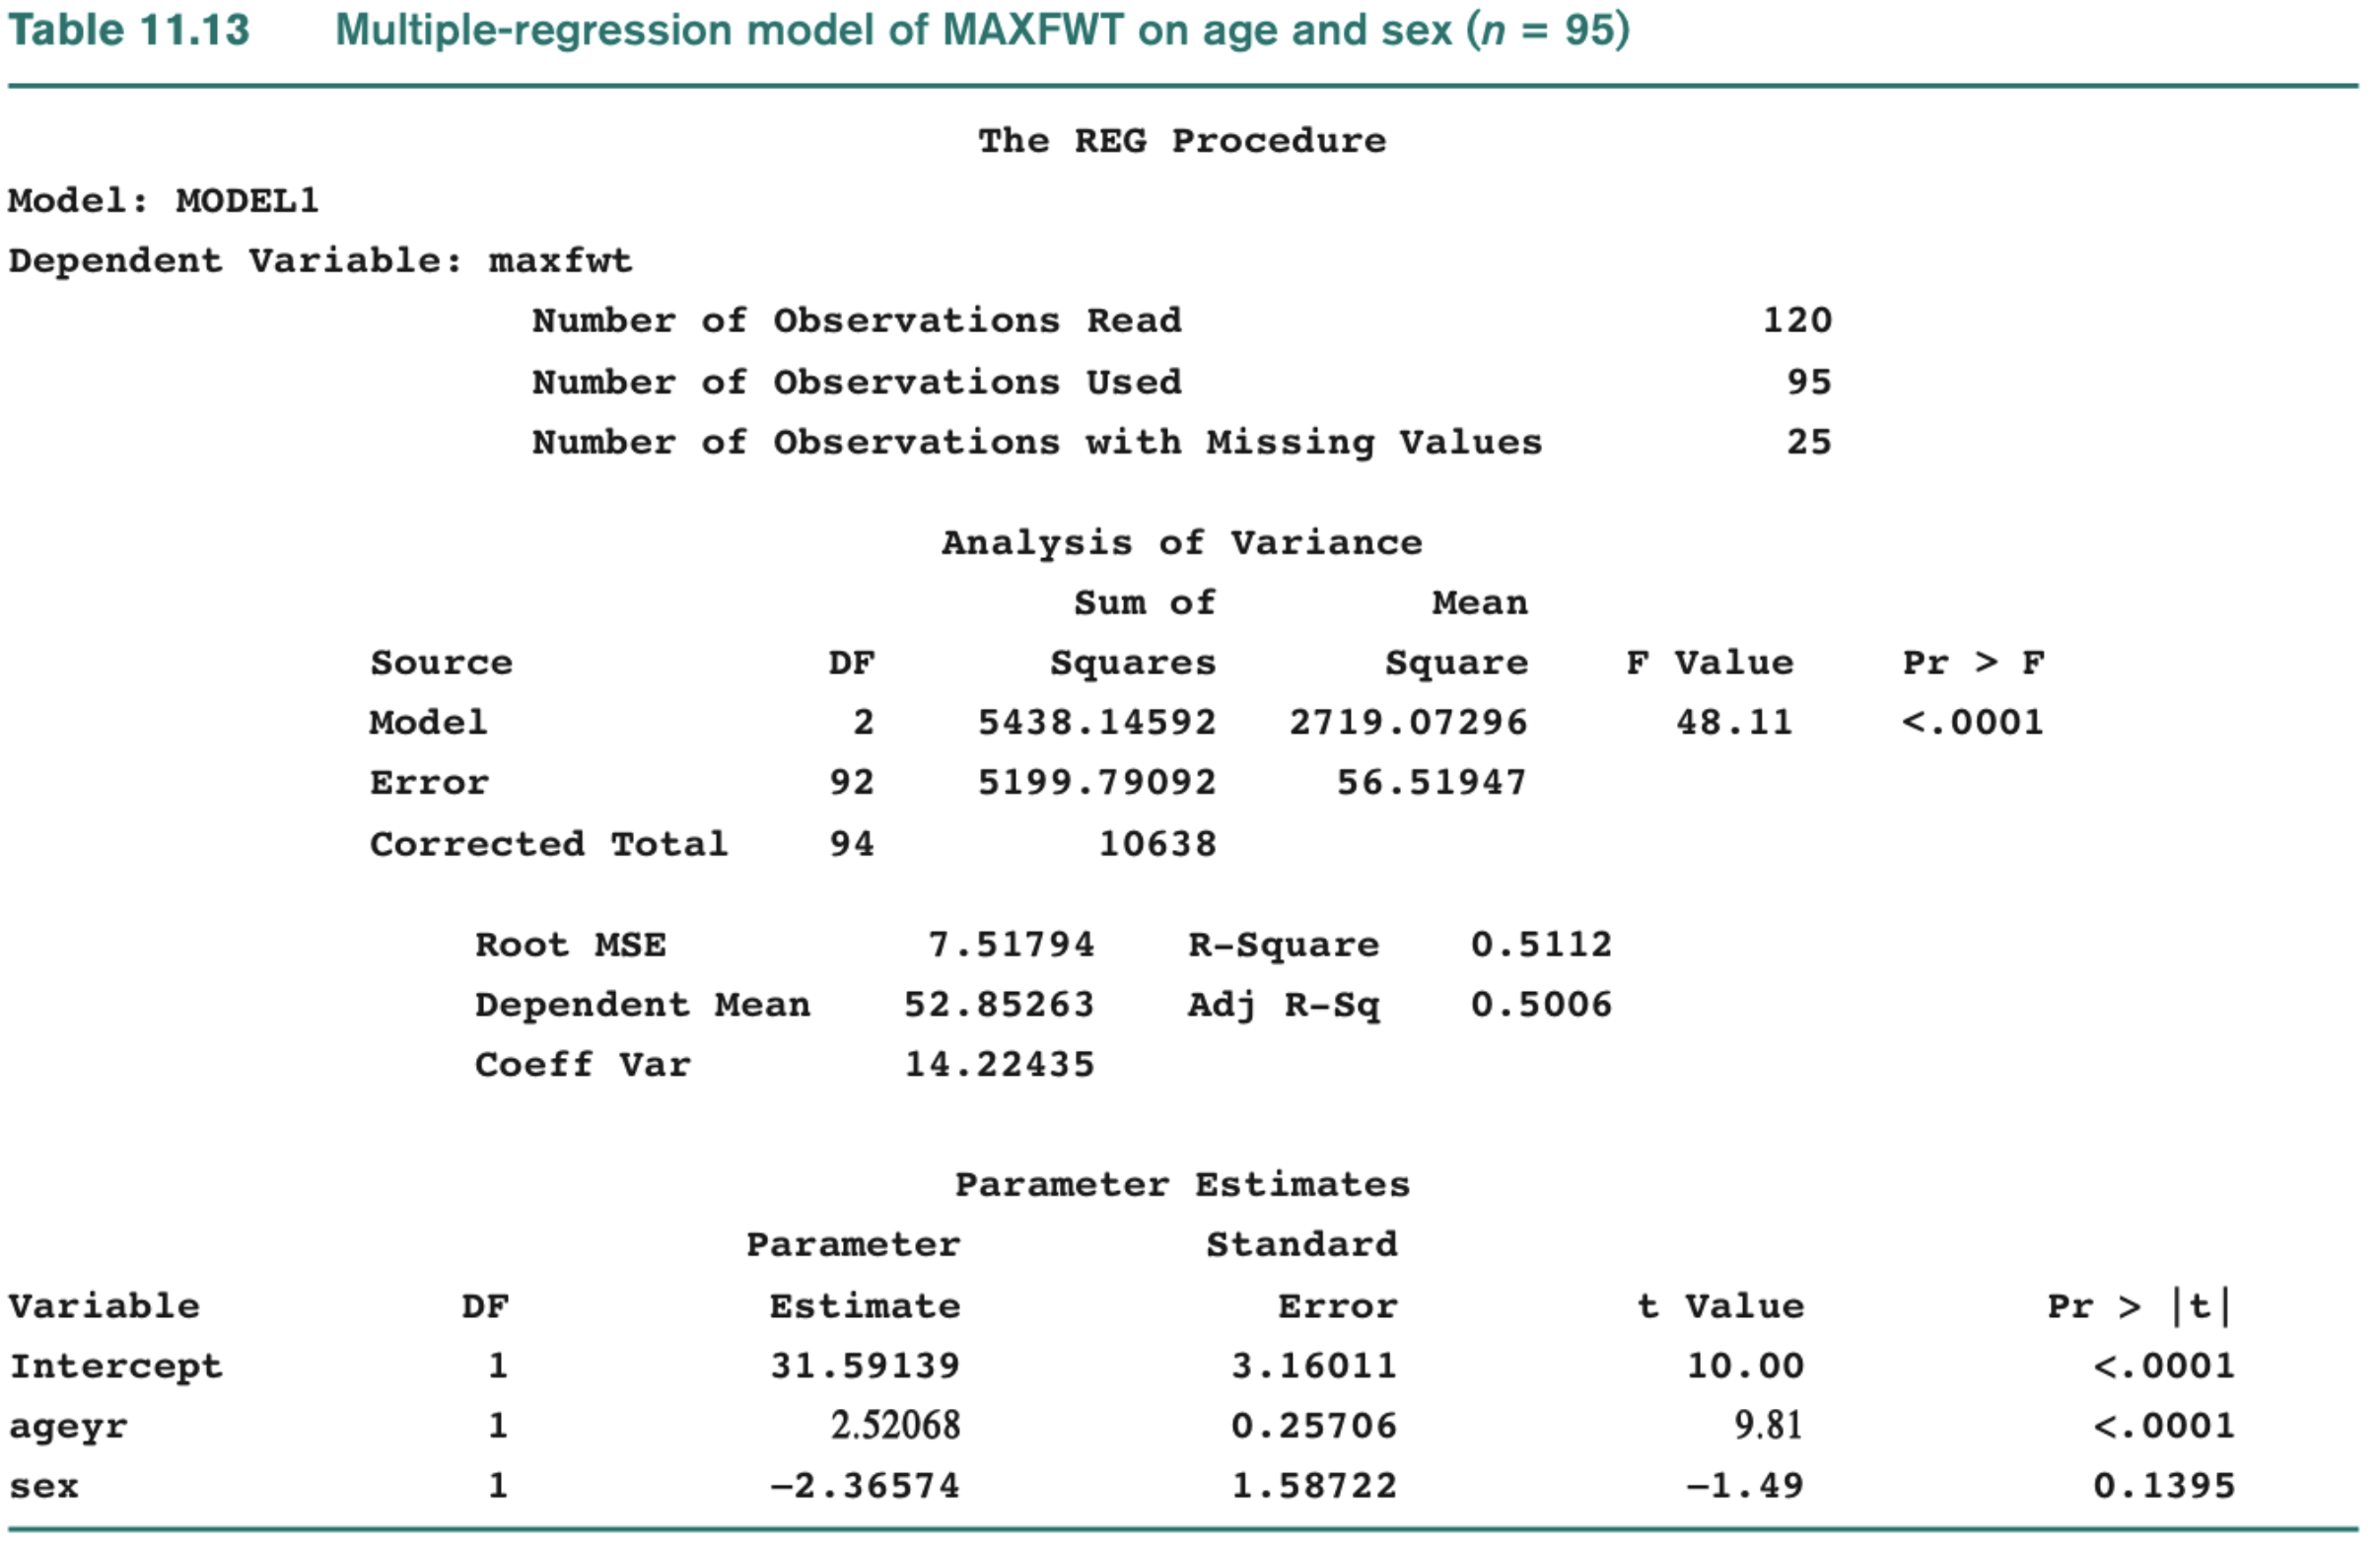
\includegraphics[width=1\textwidth]{fig26.png}
\end{figure}
\begin{figure}[H]
    \centering
    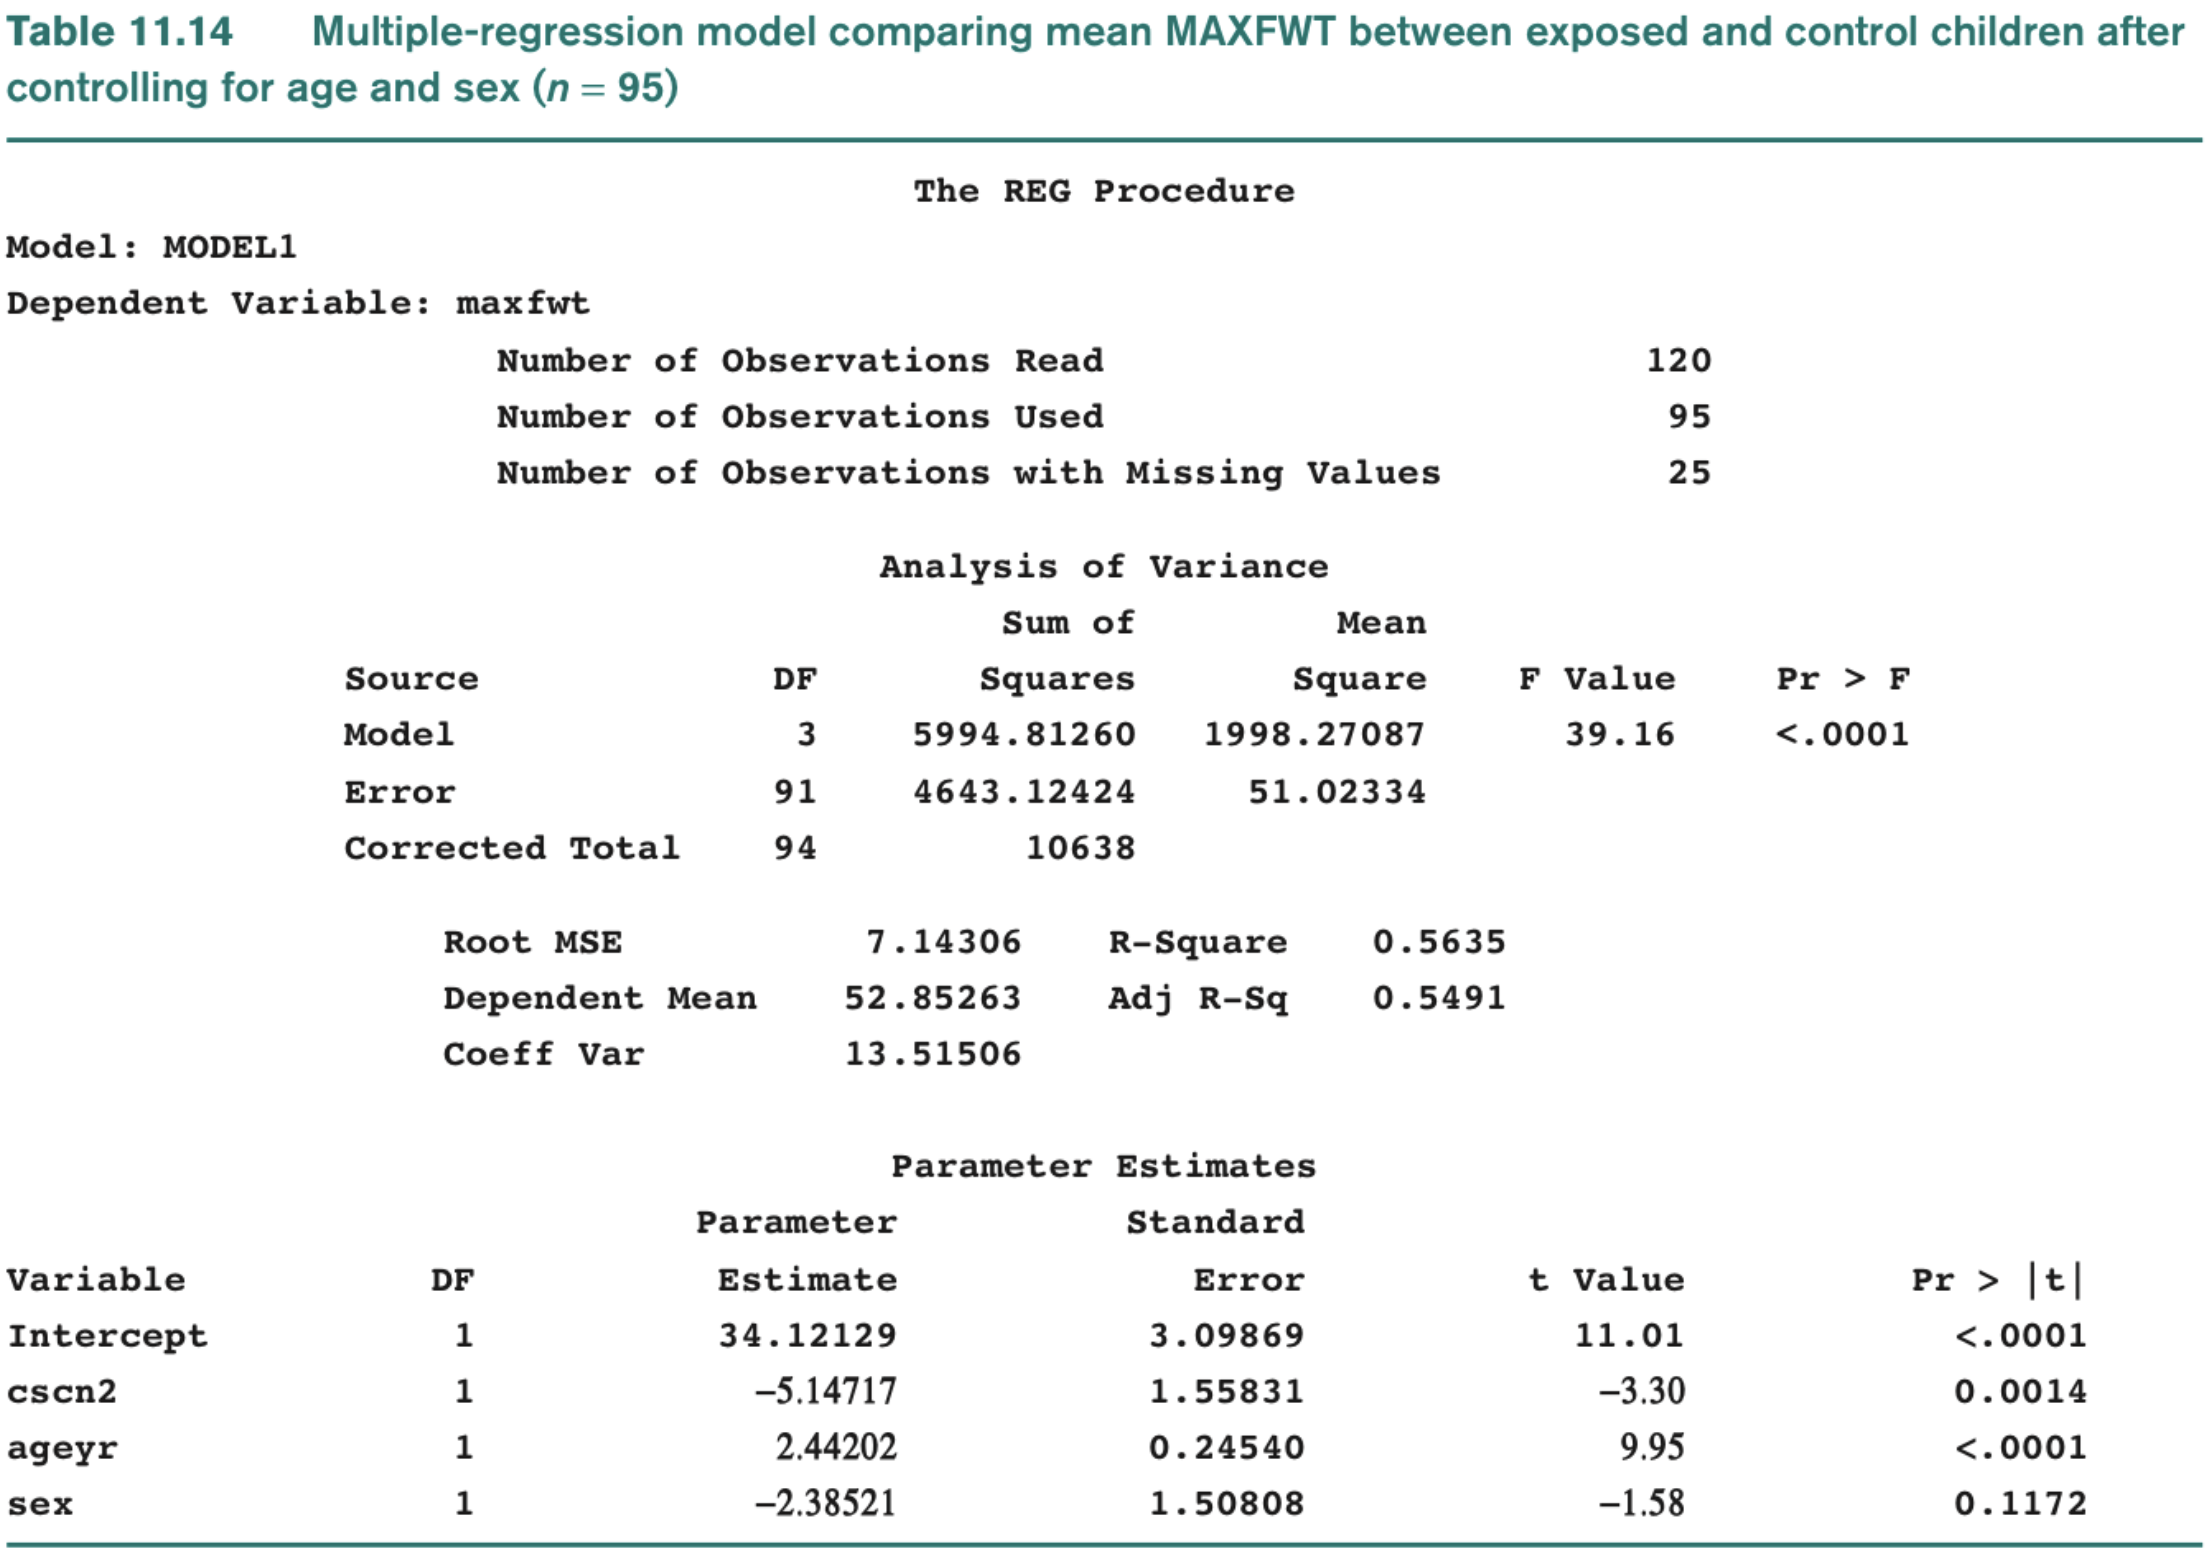
\includegraphics[width=1\textwidth]{fig27.png}
    \text{From Rosner 7th ed.}
\end{figure}

\newpage

\section*{The Main Effects Model}

Fig 5.3 suggests intercepts might differ, but slopes may be equal.
\[
\Rightarrow E(\textcolor{blue}{\text{lifeExp}} \mid \log(\textcolor{blue}{\text{ppgdp}}) = x, \, \text{group})
\]
\[
= \beta_0 + \beta_{02} U_2 + \beta_{03} U_3 + \beta_1 x
\]
\textcolor{red}{Main effects model [ no interactions ]}
\begin{figure}[H]
    \centering
    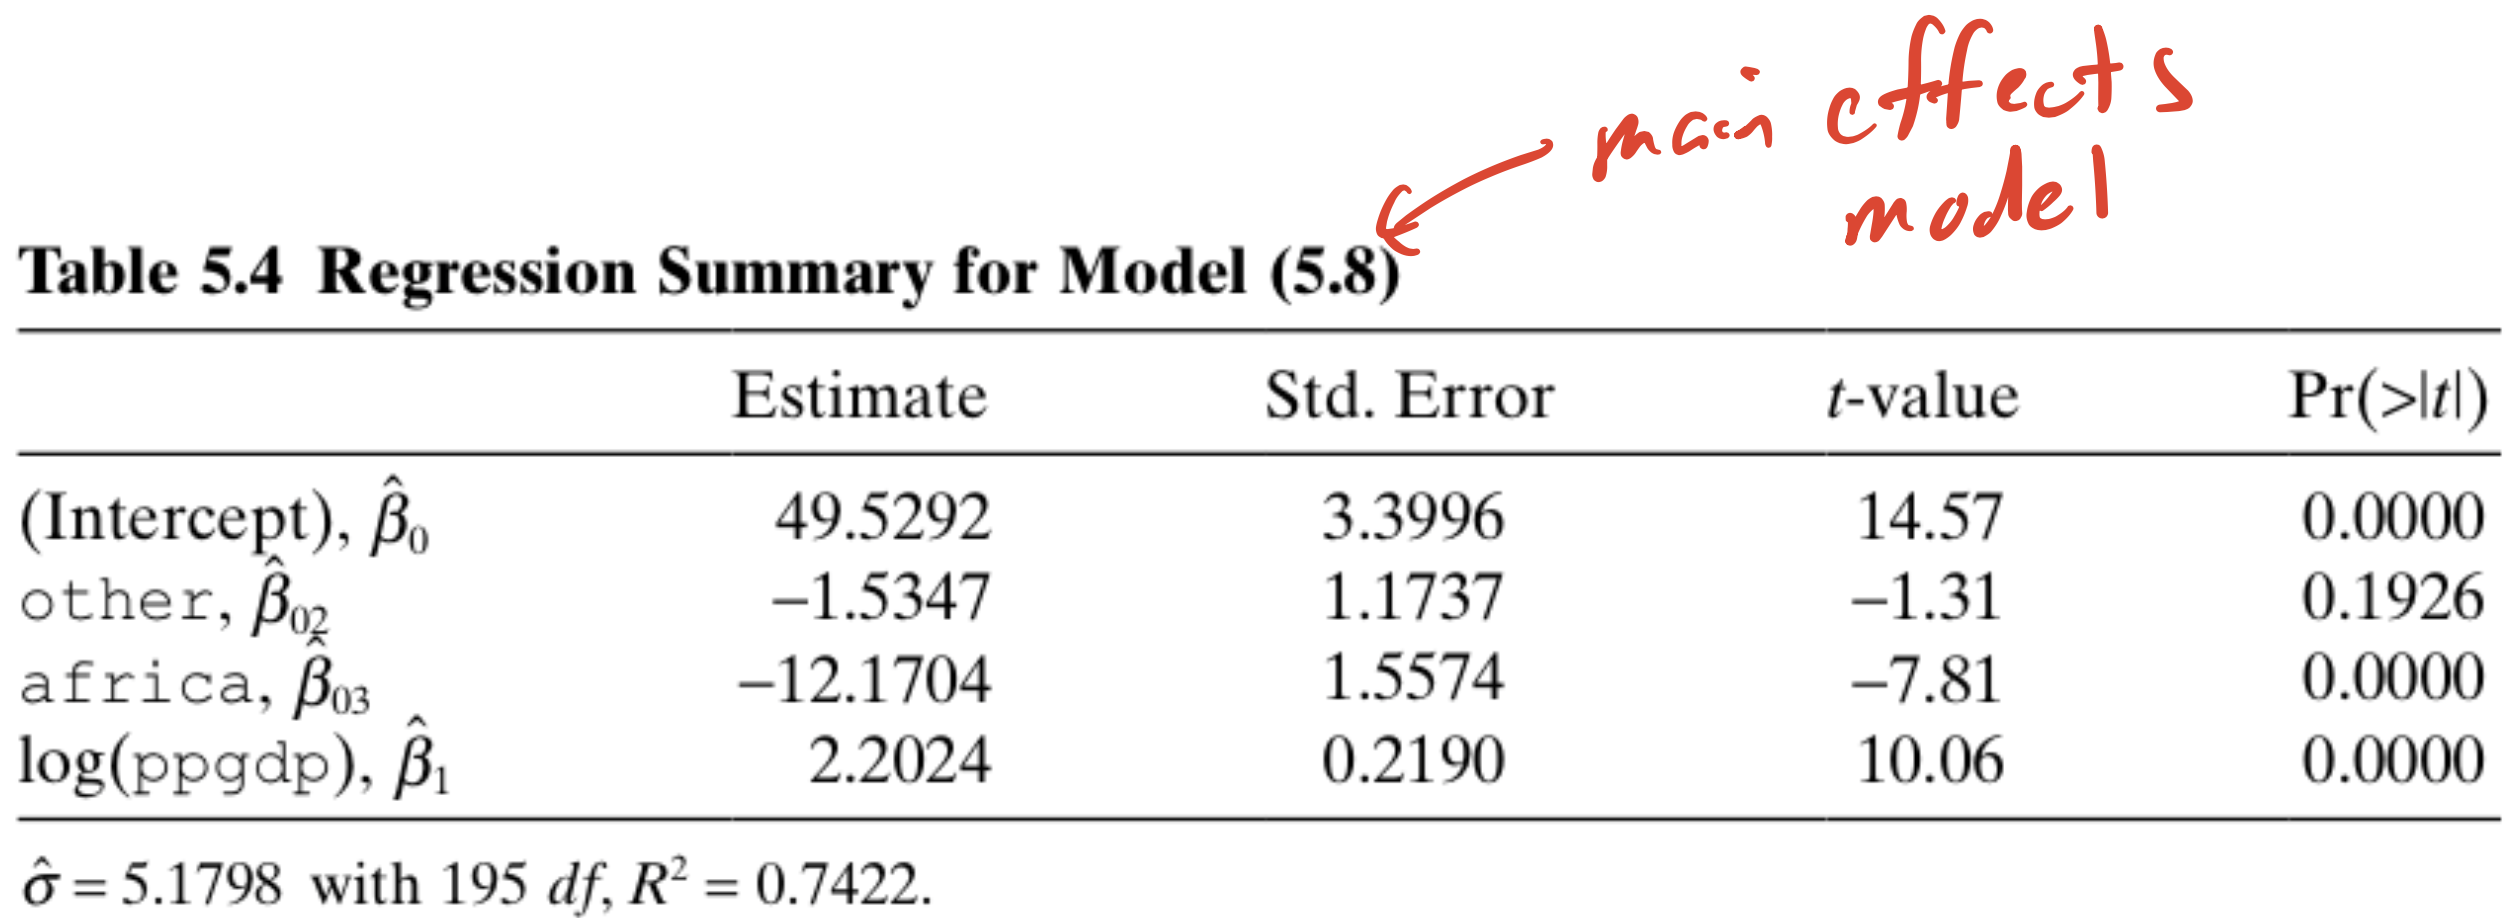
\includegraphics[width=1\textwidth]{fig28.png}
\end{figure}
\begin{figure}[H]
    \centering
    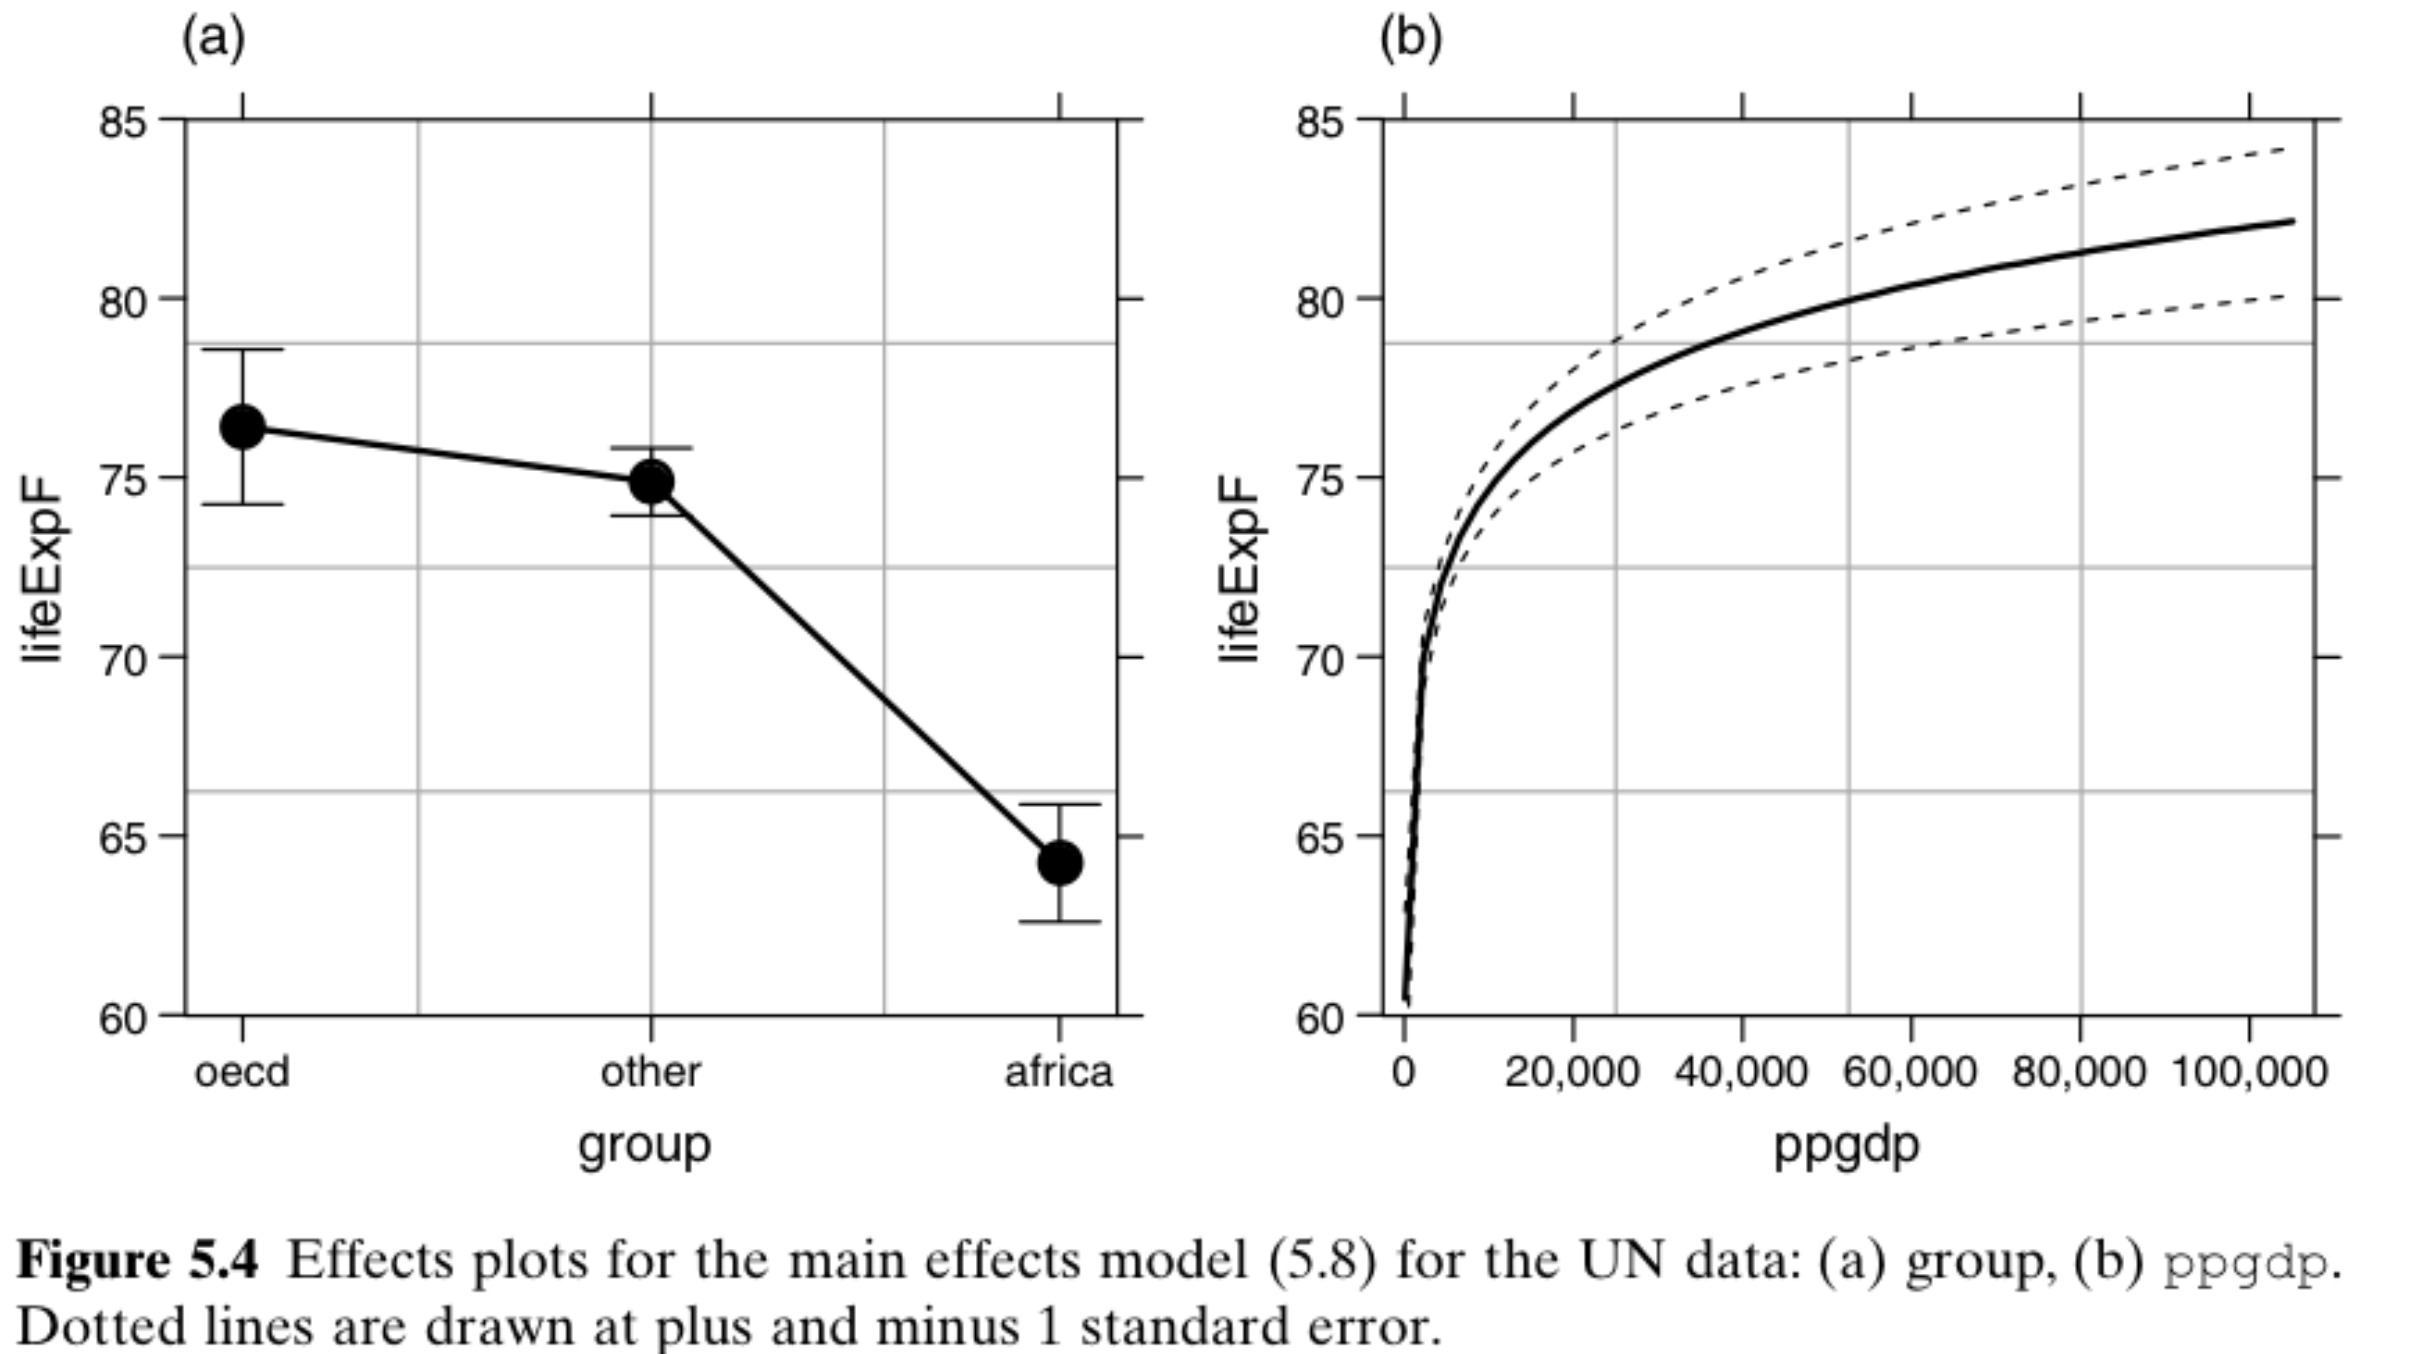
\includegraphics[width=1\textwidth]{fig29.png}
\end{figure}

\section*{Many Factors}

Let's say we have 3 factors, each with 3 possible levels.
\[
\Rightarrow 3^3 = 27 \text{ possible combinations of the three factors}
\]
\subsection*{Main effects means model}
 - Intercept and 2 dummy variables per factor \\
\textcolor{red}{$\Rightarrow$ 7 total parameters}\\

\subsection*{Second-order means model}
 - Adds in all 2-factor interactions\\
\textcolor{red}{$\Rightarrow$ Total \# parameters $7 + (3 \times 4) = 19$}\\

\subsection*{Third-order means model}
 - Includes all 3-way interactions between factors \\
\textcolor{red}{$\Rightarrow$ Total \# parameters $19 + 8 = 27$}
\vspace{1.5cm}

\noindent
These kinds of means models are called \textcolor{blue}{ANOVA}.\\
\textcolor{red}{[will discuss in more detail shortly]}

\newpage

\section*{Polynomial Regression}

Consider model:
\[
E(Y \mid X = x) = \beta_0 + \beta_1 x + \beta_2 x^2
\]
\begin{figure}[H]
    \centering
    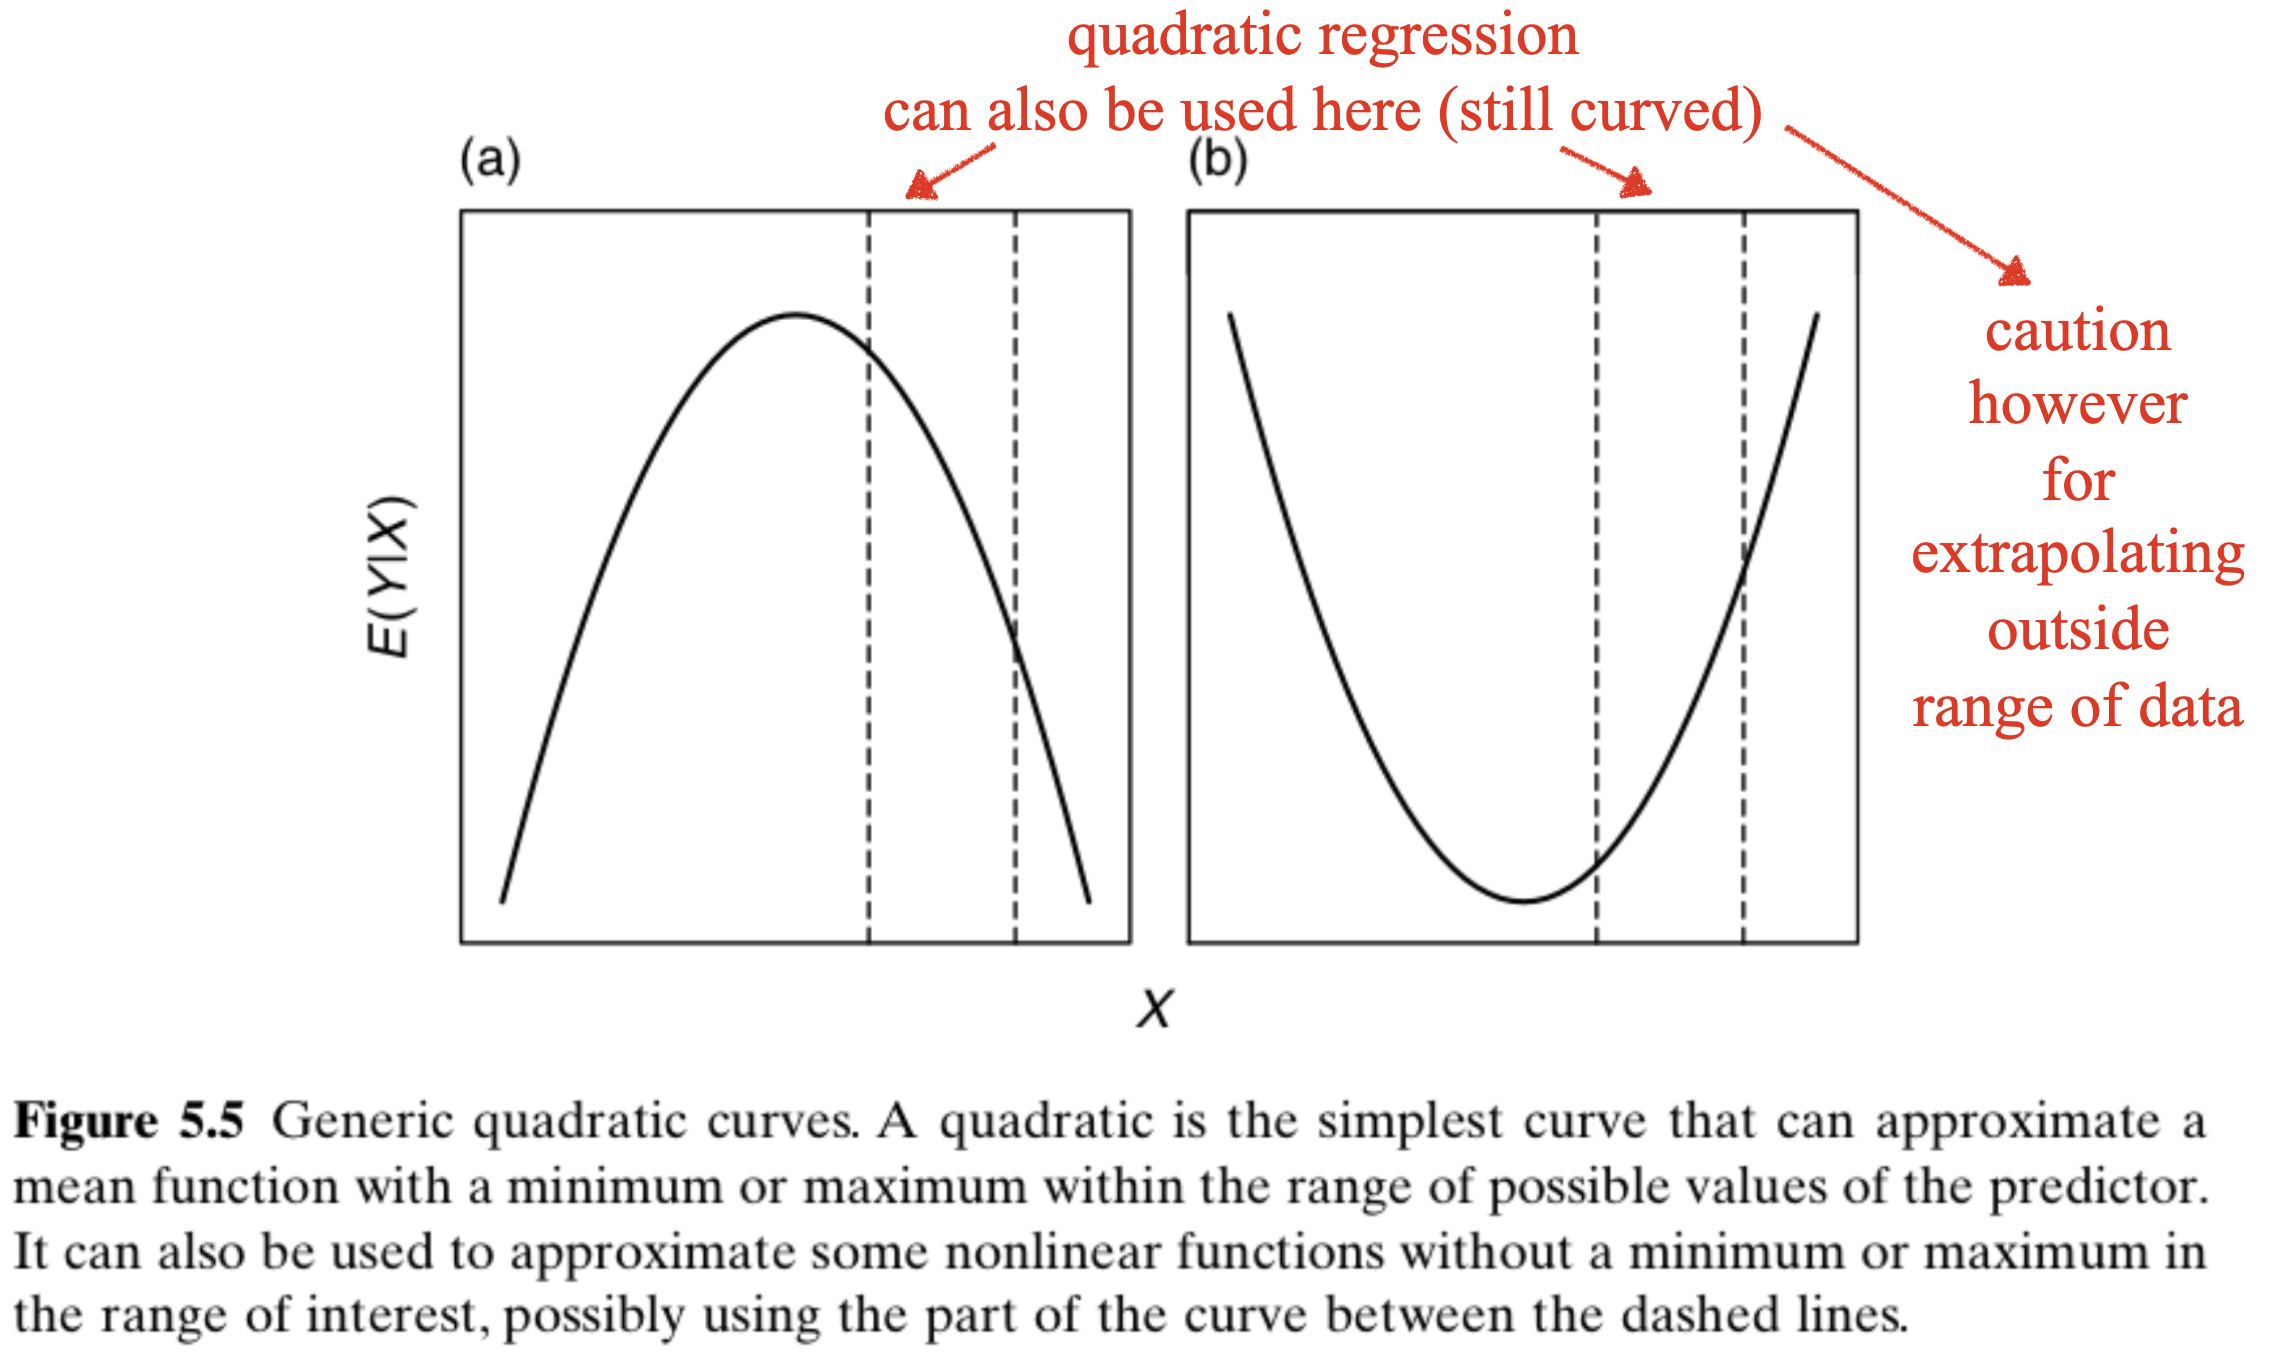
\includegraphics[width=1\textwidth]{fig30.png}
\end{figure}
\noindent
Min or Max will occur at value of $X$ where
\[
\frac{dE(Y \mid X = x)}{dx} = 0 \quad 
\Rightarrow x_{\mu} = -\frac{\beta_1}{2 \beta_2}
\]

\subsection*{Polynomial regression model}

\[
E(Y \mid X = x) = \beta_0 + \beta_1 x + \beta_2 x^2 + \cdots + \beta_d x^d
\]
\[
d = 2 \Rightarrow \text{quadratic , } d = 3 \Rightarrow \text{cubic}
\]
\noindent
\textcolor{darkgreen}{[Can approx. any smooth curve with high enough order polynomial]}

\subsection*{Polynomials With Several Predictors}

\noindent
Consider $x_1, x_2$ as predictors
\[
E(Y \mid X_1 = x_1, X_2 = x_2) = \beta_0 + \beta_1 x_1 + \beta_2 x_2 + \beta_{11} x_1^2 + \beta_{22} x_2^2 + \beta_{12} x_1 x_2
\]
\[
\textcolor{red}{x_1x_2 \text{ is multiplicative interaction}}
\]
\textcolor{blue}{With $k$ regressors, have intercept, $k$ main effects, $k(k-1)/2$ (two-way) interactions.\\
$\therefore$ with $k = 5 \Rightarrow 21$ regressors, $k = 10 \Rightarrow 66$ regressors.}\\
\textit{An illustrative example:}
\begin{figure}[H]
    \centering
    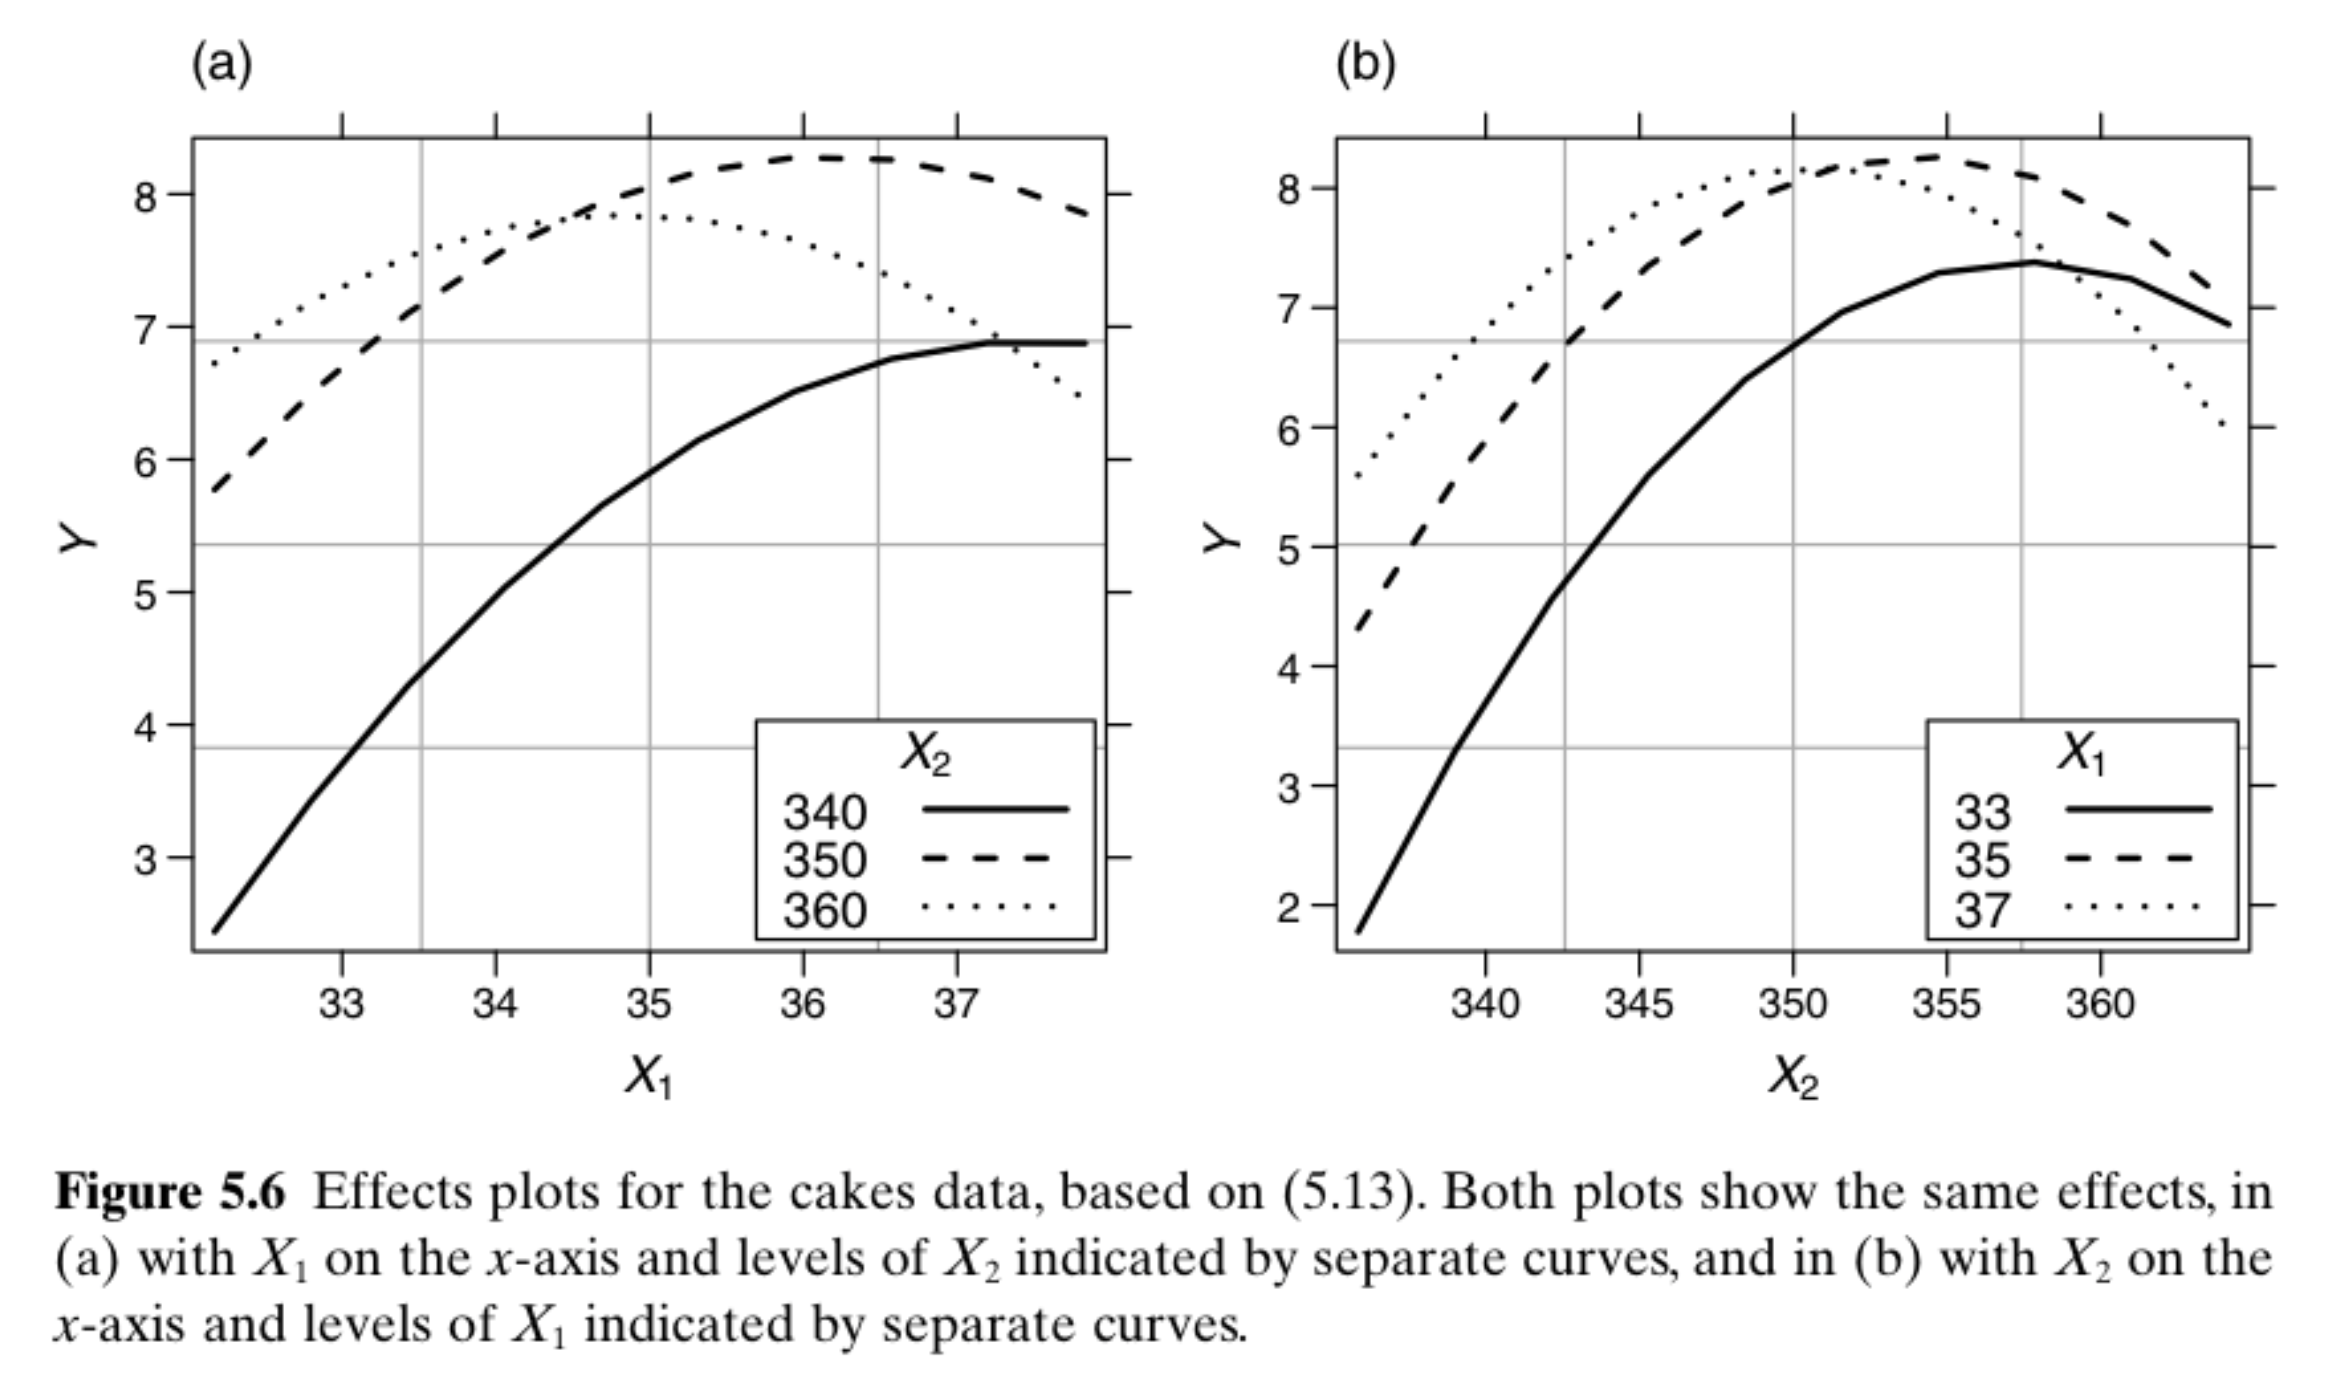
\includegraphics[width=1\textwidth]{fig31.png}
\end{figure}

\section*{Splines}

\begin{figure}[H]
    \centering
    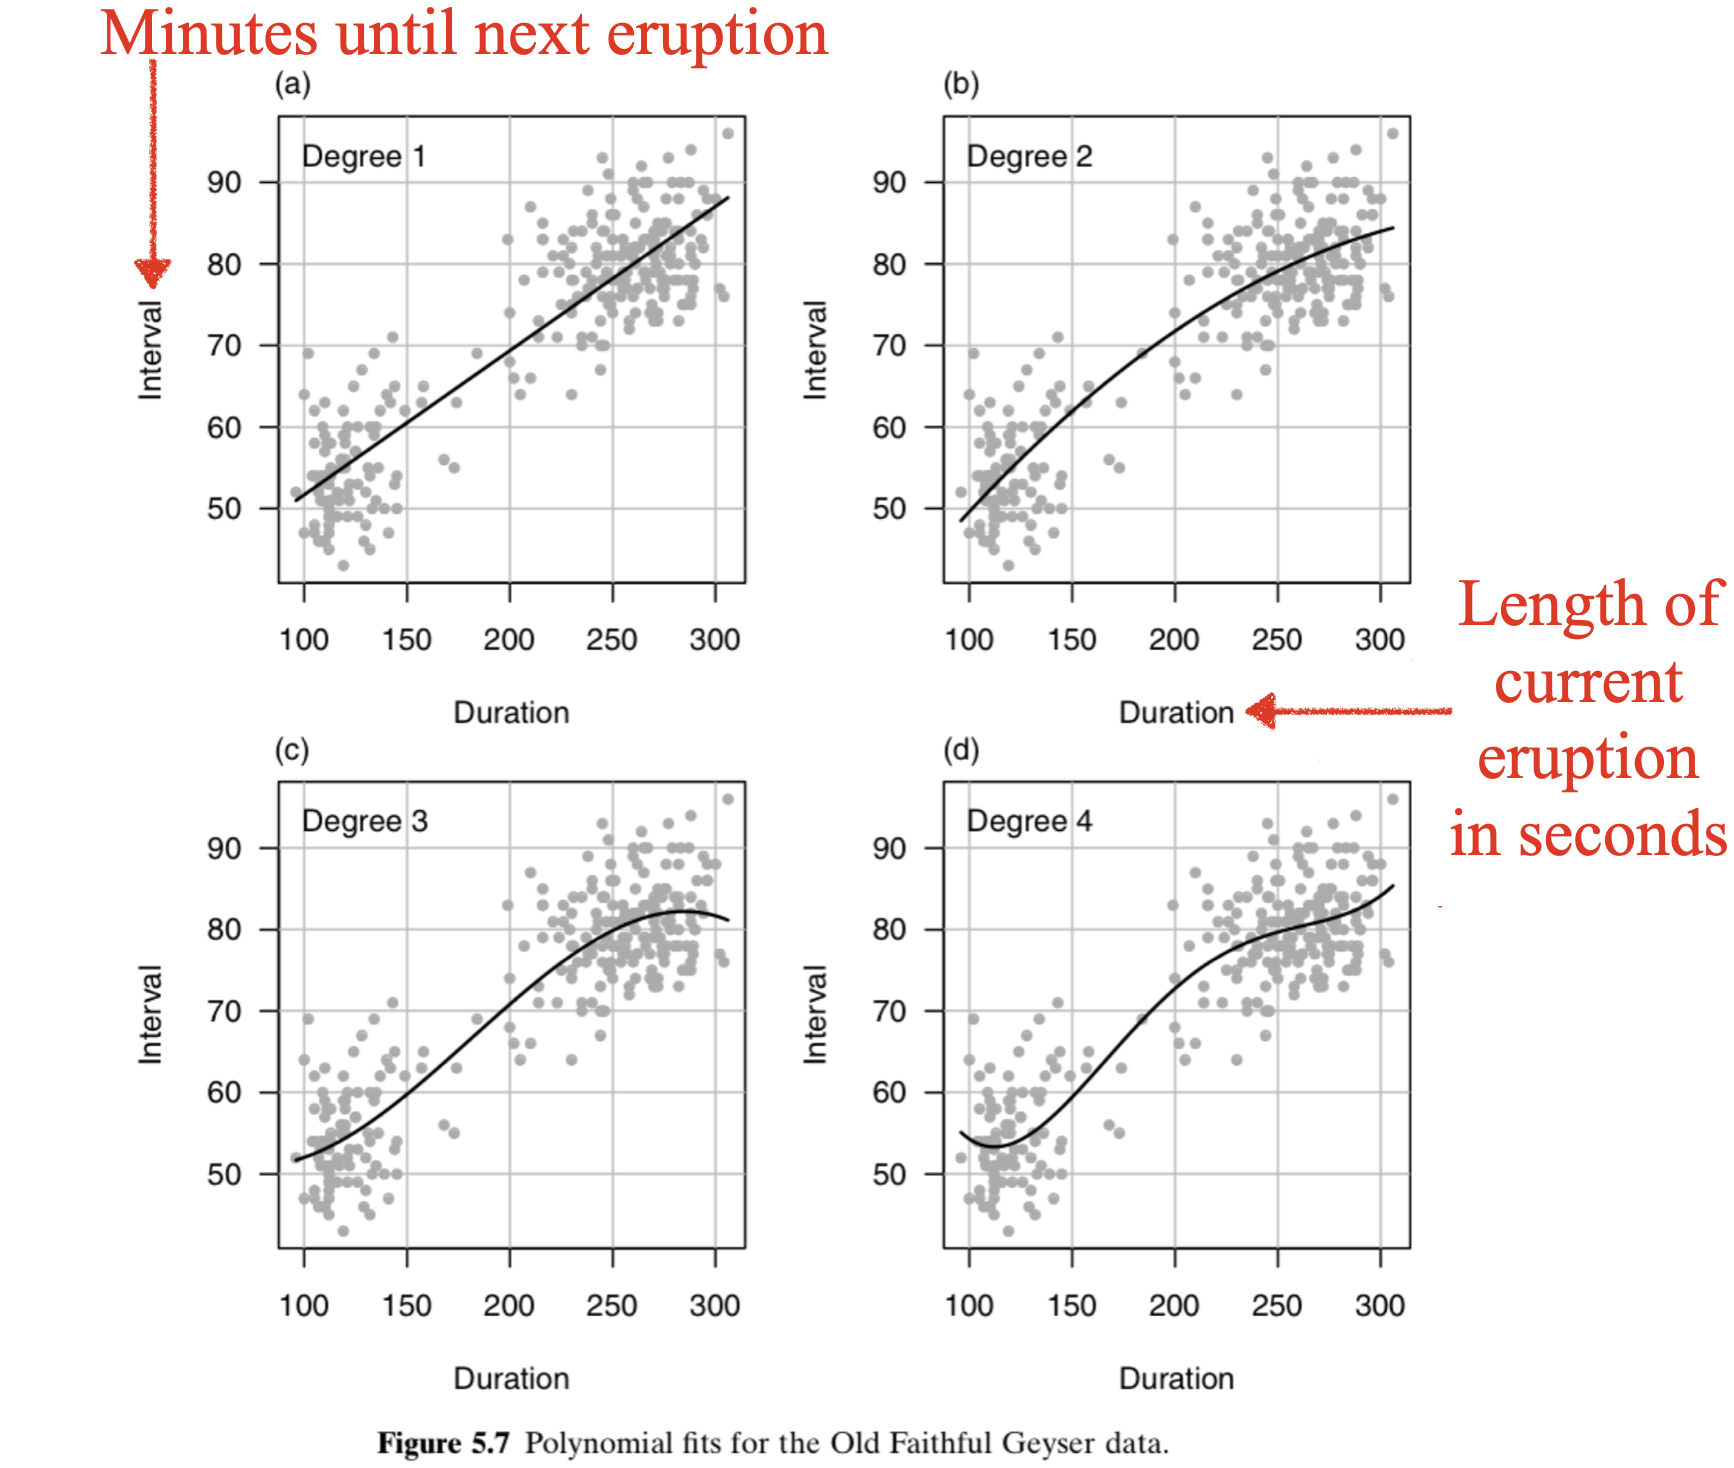
\includegraphics[width=0.95\textwidth]{fig32.png}
\end{figure}
\noindent
\textcolor{blue}{Increasing degree of polynomial can improve some aspects of fit but make others worse} \textcolor{red}{[global vs local]}.\\
\textbf{Polynomial fit is weighted sum of \textcolor{blue}{basis functions}}
\[ E(Y\mid X=x) = \beta_0 + \sum_{j=1}^{d} \beta_j x^j \]
Basis functions are monomials $\{x^1, x^2, \ldots, x^d\}$\\
Weights are $\beta$'s\\
\textcolor{red}{Useful for global fitting because defined for all possible values of $X$.}\textcolor{darkgreen}{[not local]}

\section*{Splines}

\noindent
- different set of basis functions\\
- defined locally\\
\textcolor{red}{$\Rightarrow$ changing weight of one basis function will mostly affect fitted curve only for a limited range of $X$.}
\begin{figure}[H]
    \centering
    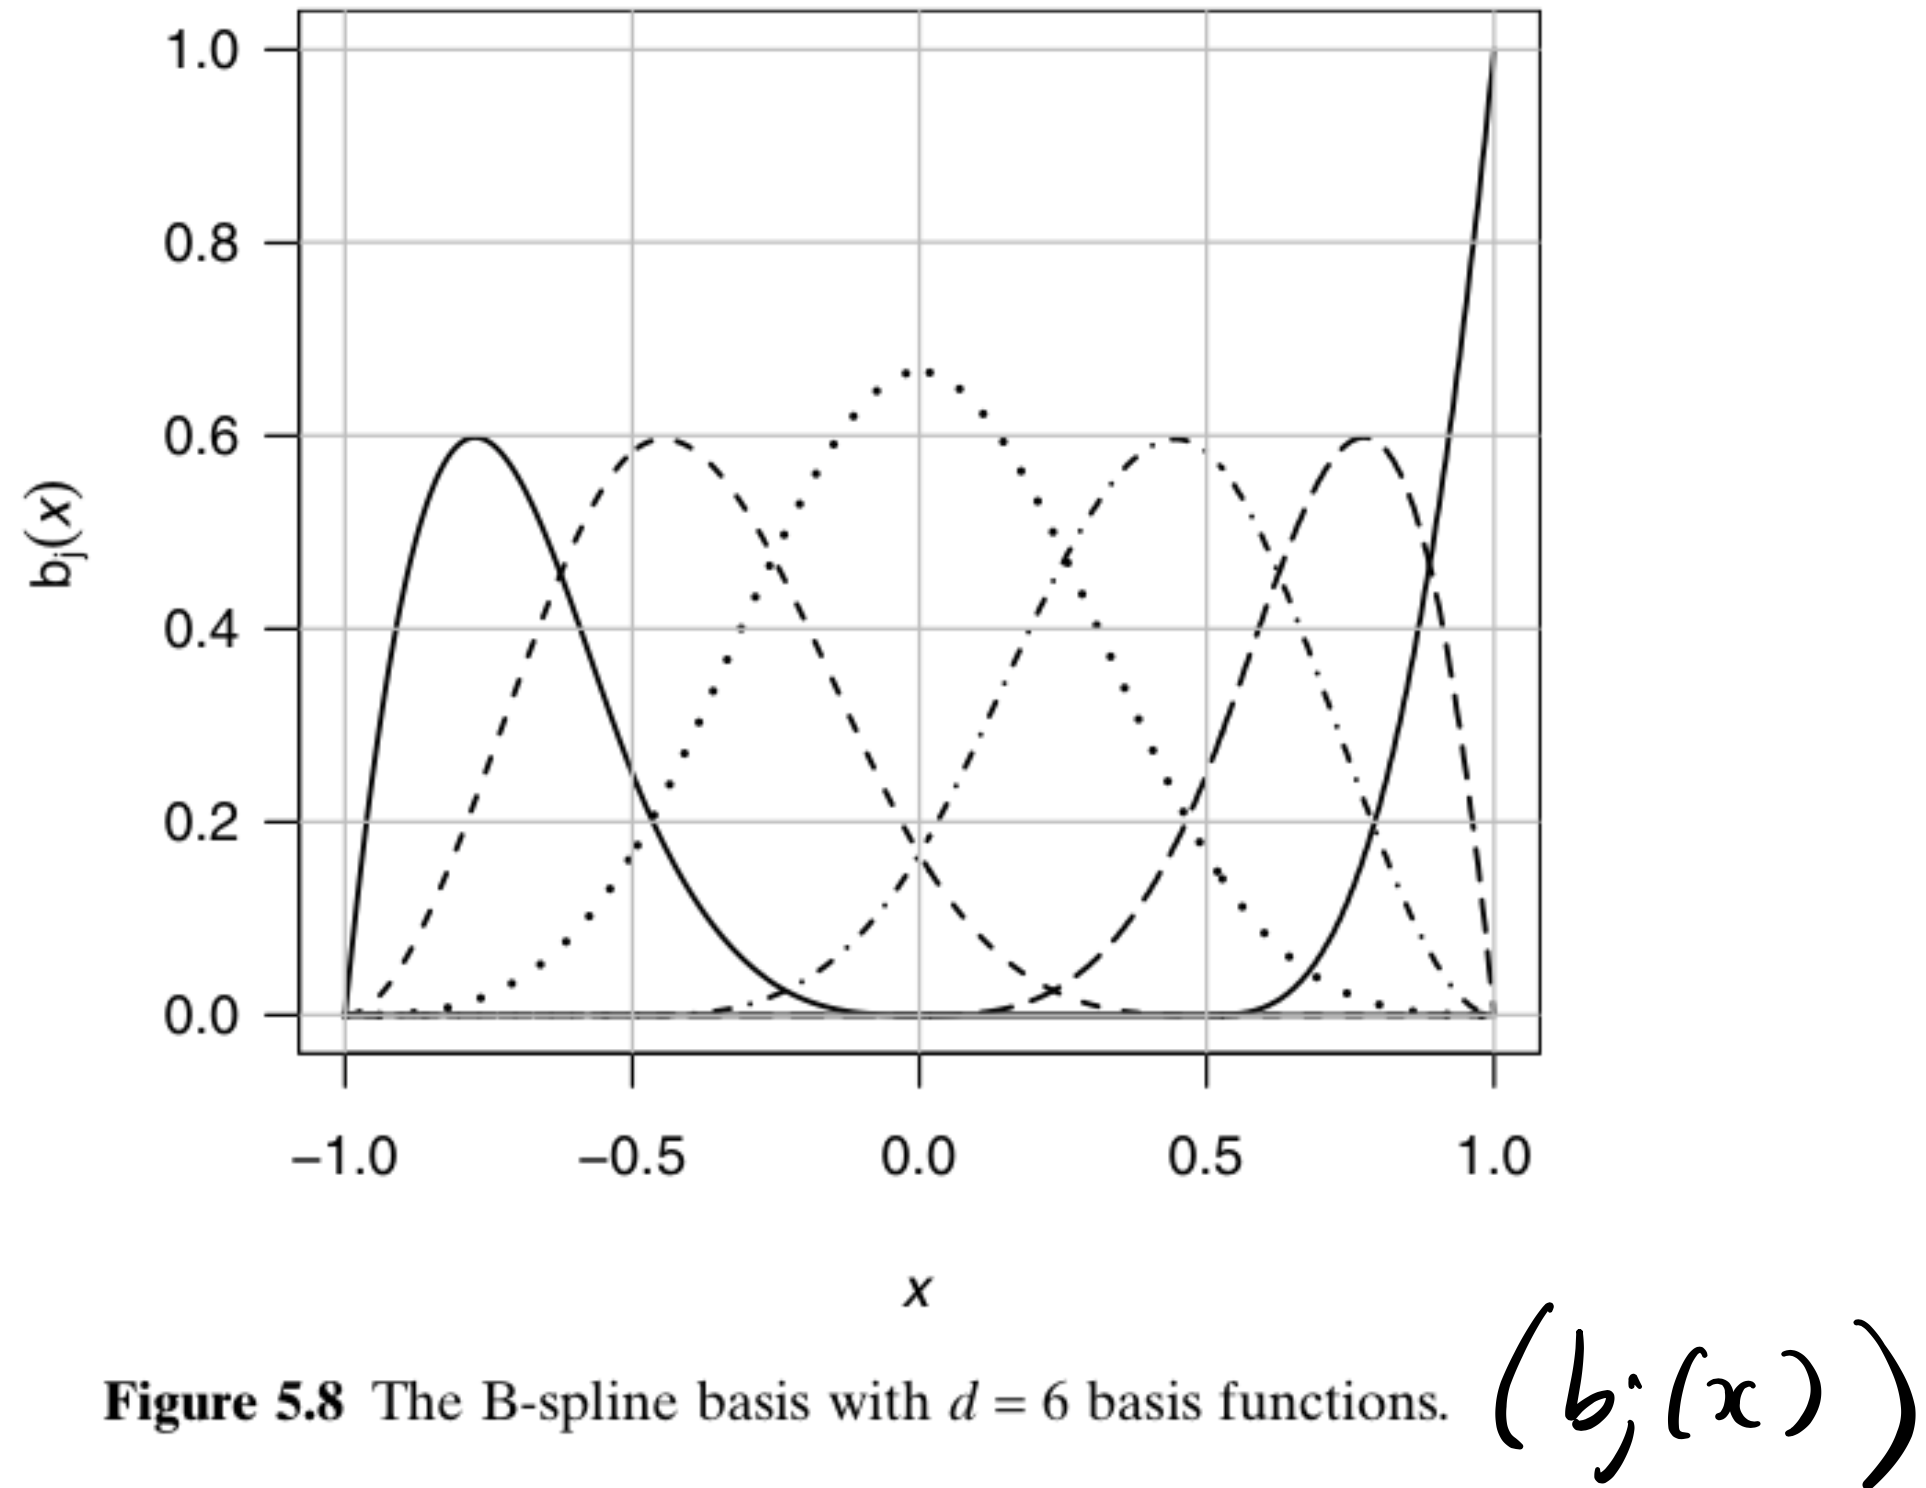
\includegraphics[width=0.95\textwidth]{fig33.png}
\end{figure}

\subsection*{General Model}

\[
E(Y \mid X = x) = \beta_0 + \sum_{j=1}^{d} \beta_j b_j(x)
\]
\begin{figure}[H]
    \centering
    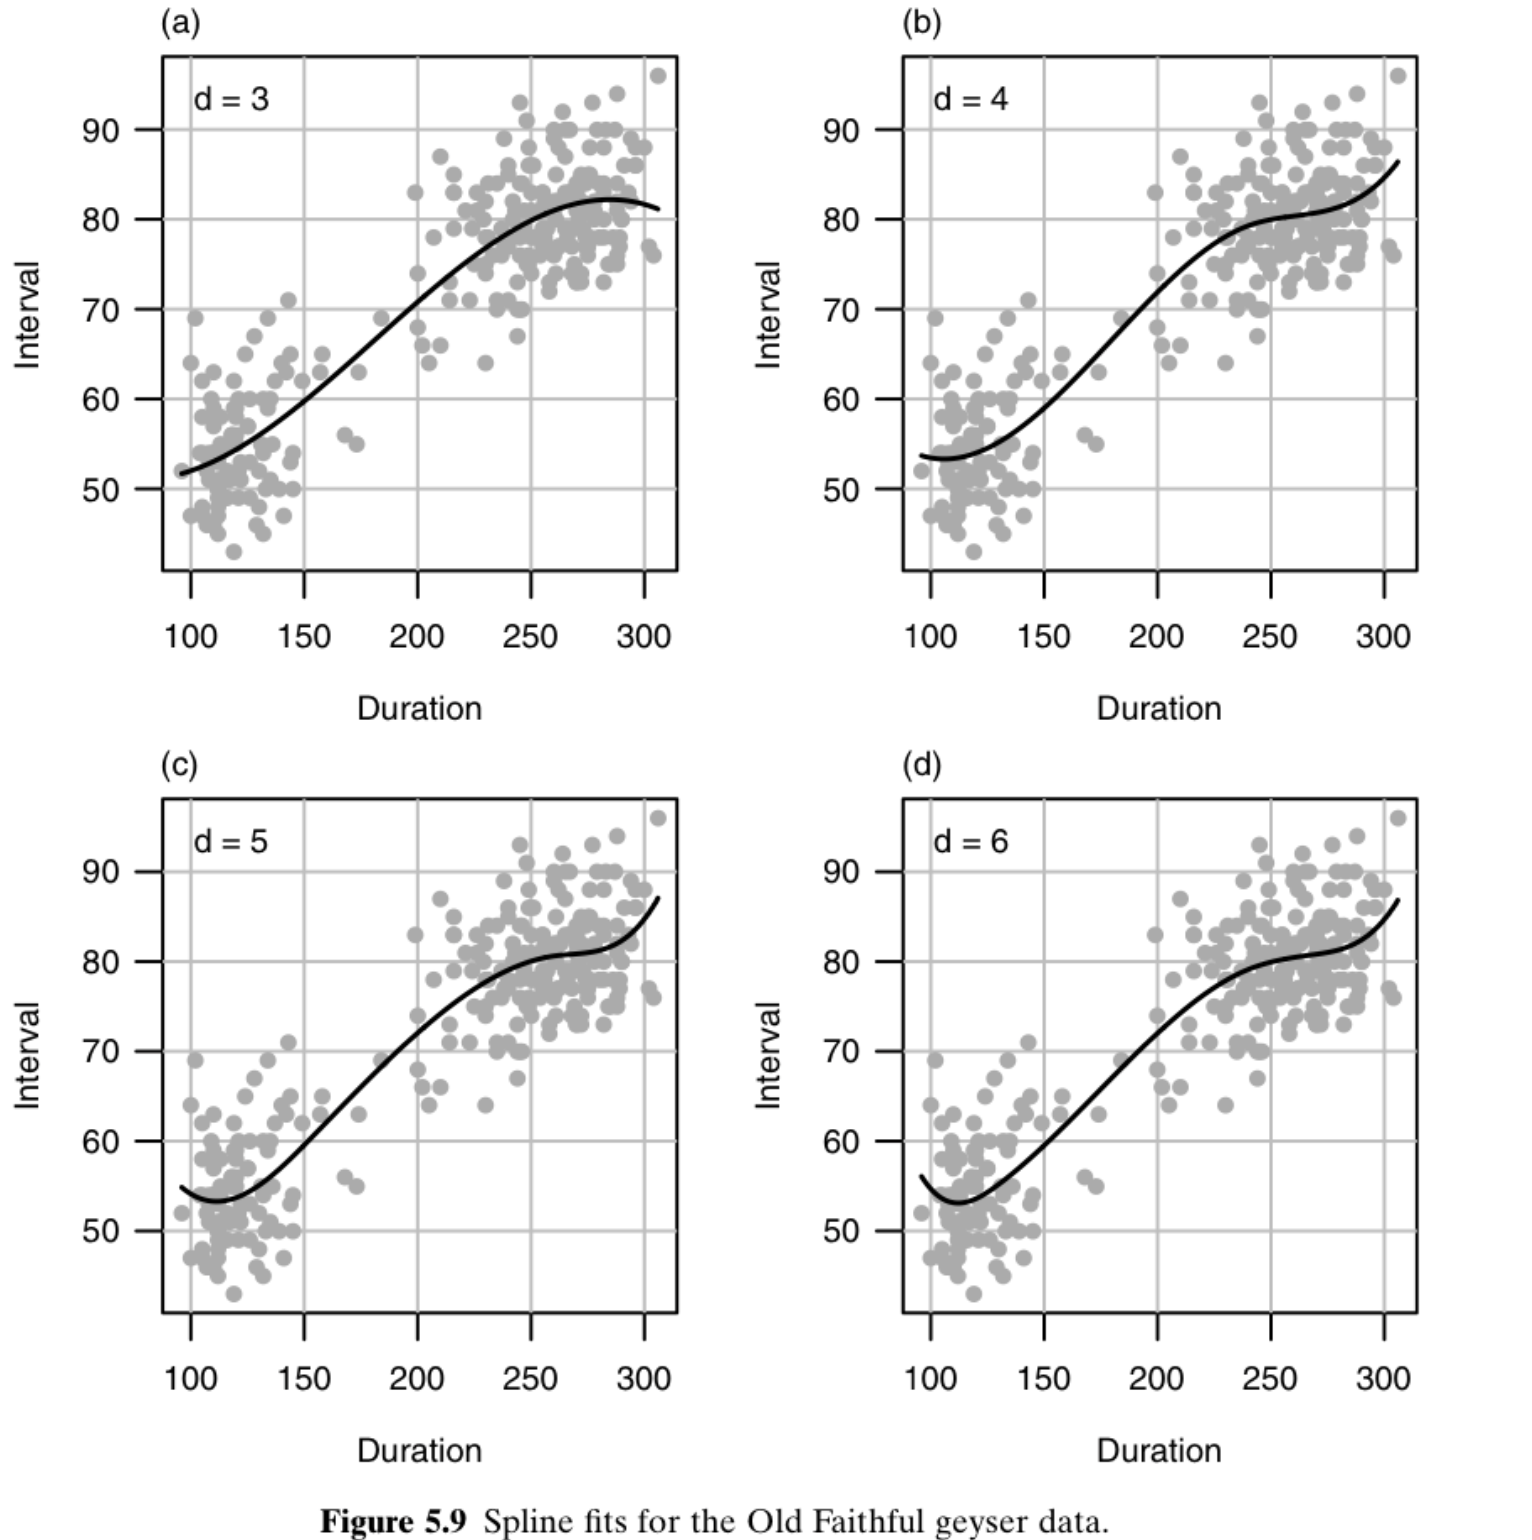
\includegraphics[width=0.95\textwidth]{fig34.png}
\end{figure}
\noindent
\textbf{How to estimate weights (coefficients)?}\\
- use OLS\\
- but degree of polynomial $d$ is a \textcolor{blue}{tuning parameter} controlling amount of smoothness.\\
\textcolor{darkgreen}{[May discuss more later]}






\end{document}